%%%%%%%%%%%%%%%%%%%%%%%%%%%%%%%%%%%%%%%%%%%%%%%%%%%%%%%%%%%%%%%%%%%%%%%%%%%%%%%%
%% MASTER'S THESIS                                                            %%
%%                                                                            %% 
%% Title (en): Multi-Agent Systems and Organizations                          %%
%% Title (cs): Multiagentní systémy a organizace                              %%
%%                                                                            %%
%% Author: Bc. Lukáš Kúdela                                                   %%
%% Supervisor: Prof. RNDr. Petr Štěpánek, DrSc.                               %%
%%                                                                            %%
%% Academic year: 2011/2012                                                   %%
%%%%%%%%%%%%%%%%%%%%%%%%%%%%%%%%%%%%%%%%%%%%%%%%%%%%%%%%%%%%%%%%%%%%%%%%%%%%%%%%

%%%%%%%%%%%%%%%%%%%%%%%%%%%%%%%%%%%%%%%%%%%%%%%%%%%%%%%%%%%%%%%%%%%%%%%%%%%%%%%%
%% Document Class                                                             %%
%%%%%%%%%%%%%%%%%%%%%%%%%%%%%%%%%%%%%%%%%%%%%%%%%%%%%%%%%%%%%%%%%%%%%%%%%%%%%%%%

\documentclass[12pt,a4paper]{report} % One-sided printing
%\documentclass[12pt,a4paper,twoside,openright]{report} % Two-sided printing

%% Page Layout %%%%%%%%%%%%%%%%%%%%%%%%%%%%%%%%%%%%%%%%%%%%%%%%%%%%%%%%%%%%%%%%%

\setlength{\textwidth}{145mm}
\setlength{\textheight}{247mm}
\setlength{\oddsidemargin}{15mm}
\setlength{\evensidemargin}{15mm} % One-sided printing
%\setlength{\evensidemargin}{0mm} % Two-sided printing
\setlength{\topmargin}{0mm}
\setlength{\headsep}{0mm}
\setlength{\headheight}{0mm}

%% Paragraph Formatting %%%%%%%%%%%%%%%%%%%%%%%%%%%%%%%%%%%%%%%%%%%%%%%%%%%%%%%%

\setlength{\parindent}{0mm}
\setlength{\parskip}{5mm}

%% Alias Definitions %%%%%%%%%%%%%%%%%%%%%%%%%%%%%%%%%%%%%%%%%%%%%%%%%%%%%%%%%%%

%
% \openright - causes the following text to begin on the right-hand side
%
\let\openright=\clearpage % One-sided printing
%\let\openright=\cleardoublepage % Two-sided printing

%%%%%%%%%%%%%%%%%%%%%%%%%%%%%%%%%%%%%%%%%%%%%%%%%%%%%%%%%%%%%%%%%%%%%%%%%%%%%%%%
%% Packages                                                                   %%
%%%%%%%%%%%%%%%%%%%%%%%%%%%%%%%%%%%%%%%%%%%%%%%%%%%%%%%%%%%%%%%%%%%%%%%%%%%%%%%%

%% Encoding and multilingual support %%%%%%%%%%%%%%%%%%%%%%%%%%%%%%%%%%%%%%%%%%%

% Accept different input encodings.
\usepackage[utf8]{inputenc}

%% Standard package for selecting font encodings.
%\usepackage[T1]{fontenc}

% Multilingual support for Plain TeX or LaTeX.
\usepackage[english,slovak]{babel}

\usepackage{aeguill}

%% Formatting %%%%%%%%%%%%%%%%%%%%%%%%%%%%%%%%%%%%%%%%%%%%%%%%%%%%%%%%%%%%%%%%%%

\usepackage{verbatim}

%% Flexible and complete interface to document dimensions.
%\usepackage[left=4cm]{geometry}

%% "Wide" a4 layout.
%\usepackage{a4wide}

%% Graphics %%%%%%%%%%%%%%%%%%%%%%%%%%%%%%%%%%%%%%%%%%%%%%%%%%%%%%%%%%%%%%%%%%%%

% Enhanced support for graphics.
\usepackage{graphicx}

% Convert EPS to 'encapsulated' PDF using GhostScript.
\usepackage{epstopdf}

\usepackage{float}

\usepackage{color}
\definecolor{purple}{RGB}{200,0,150}
\definecolor{blue}{RGB}{0,0,255}
\definecolor{yellow}{RGB}{230,230,0}
\definecolor{red}{RGB}{255,0,0}
\definecolor{black}{RGB}{0,0,0}
\definecolor{magenta}{RGB}{255,0,255}
\definecolor{cyan}{RGB}{0,255,255}
\definecolor{pink}{RGB}{255,175,175}
\definecolor{teal}{RGB}{0,200,150}
\definecolor{green}{RGB}{0,255,0}

%% AMS packages %%%%%%%%%%%%%%%%%%%%%%%%%%%%%%%%%%%%%%%%%%%%%%%%%%%%%%%%%%%%%%%%

% AMS mathematical facilities for LaTeX.
\usepackage{amsmath}

% Typesetting theorems (AMS style).
\usepackage{amsthm}

\usepackage{amssymb}

% TeX fonts from the American Mathematical Society.
\usepackage{amsfonts}

%% Micellaneous %%%%%%%%%%%%%%%%%%%%%%%%%%%%%%%%%%%%%%%%%%%%%%%%%%%%%%%%%%%%%%%%

% Make PDF files searchable and copyable.
\usepackage{cmap}

% Verbatim with URL-sensitive line breaks.
\usepackage{url}

%% Extensive support for hypertext in LaTeX.
%\usepackage[ps2pdf,unicode]{hyperref} % URL: 
%\hypersetup{pdftitle=Multi-Agent Systems and Organizations}
%\hypersetup{pdfauthor=Lukáš Kúdela}

\usepackage[htt]{hyphenat}

%%%%%%%%%%%%%%%%%%%%%%%%%%%%%%%%%%%%%%%%%%%%%%%%%%%%%%%%%%%%%%%%%%%%%%%%%%%%%%%%
%% Command & Environment Definitions                                          %%
%%%%%%%%%%%%%%%%%%%%%%%%%%%%%%%%%%%%%%%%%%%%%%%%%%%%%%%%%%%%%%%%%%%%%%%%%%%%%%%%

%
% \chapwithtoc - Starts a unnumbered chapter included in the TOC.
%
\newcommand{\chapwithtoc}[1]{
	\chapter*{#1}
	\addcontentsline{toc}{chapter}{#1}
}

%
% \comments - Inserts a inline comment.
%
\newcommand{\comments}[1]{}

%
% \stereotype - Inserts a UML stereotype.
%
\newcommand{\stereotype}[1]{
	\guillemotleft {#1}\guillemotright
}

%%%%%%%%%%%%%%%%%%%%%%%%%%%%%%%%%%%%%%%%%%%%%%%%%%%%%%%%%%%%%%%%%%%%%%%%%%%%%%%%
%% Document                                                                   %%
%%%%%%%%%%%%%%%%%%%%%%%%%%%%%%%%%%%%%%%%%%%%%%%%%%%%%%%%%%%%%%%%%%%%%%%%%%%%%%%%

\begin{document}

% Select English as the default language.
\selectlanguage{english}
\nonfrenchspacing

%% Top Matter %%%%%%%%%%%%%%%%%%%%%%%%%%%%%%%%%%%%%%%%%%%%%%%%%%%%%%%%%%%%%%%%%%

%% Standard title page
%\title{Multi-Agent Systems and Organizations}
%\author{Lukáš Kúdela}
%\maketitle

% Custom title page 
%%%%%%%%%%%%%%%%%%%%%%%%%%%%%%%%%%%%%%%%%%%%%%%%%%%%%%%%%%%%%%%%%%%%%%%%%%%%%%%%
%% MASTER'S THESIS                                                            %%
%%                                                                            %% 
%% Title (en): Multi-Agent Systems and Organizations                          %%
%% Title (cs): Multiagentní systémy a organizace                              %%
%%                                                                            %%
%% Author: Bc. Lukáš Kúdela                                                   %%
%% Supervisor: Prof. RNDr. Petr Štěpánek, DrSc.                               %%
%%                                                                            %%
%% Academic year: 2011/2012                                                   %%
%%%%%%%%%%%%%%%%%%%%%%%%%%%%%%%%%%%%%%%%%%%%%%%%%%%%%%%%%%%%%%%%%%%%%%%%%%%%%%%%

\begin{titlepage}
\begin{center}

% University
\large
Charles University in Prague

\medskip

% Faculty
Faculty of Mathematics and Physics

\vfill

{\Large \textbf{MASTER'S THESIS}}

\vfill

% MFF logo

\includegraphics[width=60mm]{images/mff_logo.eps}

\vfill
\vspace{5mm}

% Author
{\LARGE Bc. Lukáš Kúdela}

\vspace{15mm}

{\LARGE \textbf{Multi-Agent Systems and Organizations}}

\vfill

% Department
Department of Theoretical Computer Science and Mathematical Logic

\vfill

\begin{tabular}{rl}
Thesis supervisor: & Prof. RNDr. Petr Štěpánek, DrSc.\\
\noalign{\vspace{2mm}}
Study programme: & Computer Science (N1801)\\
\noalign{\vspace{2mm}}
Specialization: & Theoretical Computer Science (1801T010)\\
\end{tabular}

\vfill

% Place and year
Prague 2012

\end{center}
\end{titlepage}

%% Body %%%%%%%%%%%%%%%%%%%%%%%%%%%%%%%%%%%%%%%%%%%%%%%%%%%%%%%%%%%%%%%%%%%%%%%%

% Page numbering off
\pagenumbering{gobble}

%%%%%%%%%%%%%%%%%%%%%%%%%%%%%%%%%%%%%%%%%%%%%%%%%%%%%%%%%%%%%%%%%%%%%%%%%%%%%%%
%% Title (en): Multiagent Systems and Organizations                          %%
%% Title (cs): Multiagentní systémy a organizace                             %%
%%                                                                           %%
%% Author: Bc. Lukáš Kúdela                                                  %%
%% Supervisor: Prof. RNDr. Petr Štěpánek, DrSc.                              %%
%%                                                                           %%
%% Academic year: 2011/2012                                                  %%
%%%%%%%%%%%%%%%%%%%%%%%%%%%%%%%%%%%%%%%%%%%%%%%%%%%%%%%%%%%%%%%%%%%%%%%%%%%%%%%

\noindent
I would like to express my gratitude ...
%%%%%%%%%%%%%%%%%%%%%%%%%%%%%%%%%%%%%%%%%%%%%%%%%%%%%%%%%%%%%%%%%%%%%%%%%%%%%%%%
%% MASTER'S THESIS                                                            %%
%%                                                                            %% 
%% Title (en): Multi-Agent Systems and Organizations                          %%
%% Title (cs): Multiagentní systémy a organizace                              %%
%%                                                                            %%
%% Author: Bc. Lukáš Kúdela                                                   %%
%% Supervisor: Prof. RNDr. Petr Štěpánek, DrSc.                               %%
%%                                                                            %%
%% Academic year: 2011/2012                                                   %%
%%%%%%%%%%%%%%%%%%%%%%%%%%%%%%%%%%%%%%%%%%%%%%%%%%%%%%%%%%%%%%%%%%%%%%%%%%%%%%%%

\vspace*{\fill}

I declare that I carried out this master thesis independently, and only with the cited sources, literature and other professional sources.

\medskip

I understand that my work relates to the rights and obligations under the Act No. 121/2000 Coll., the Copyright Act, as amended, in particular the fact that the Charles University in Prague has the right to conclude a license agreement on the use of this work as a school work pursuant to Section 60 paragraph 1 of the Copyright Act.

\bigskip

Prague, \today \hspace{\fill}Lukáš Kúdela
%%%%%%%%%%%%%%%%%%%%%%%%%%%%%%%%%%%%%%%%%%%%%%%%%%%%%%%%%%%%%%%%%%%%%%%%%%%%%%%%
%% Title (en): Multiagent Systems and Organizations                           %%
%% Title (cs): Multiagentní systémy a organizace                              %%
%%                                                                            %%
%% Author: Bc. Lukáš Kúdela                                                   %%
%% Supervisor: Prof. RNDr. Petr Štěpánek, DrSc.                               %%
%%                                                                            %%
%% Academic year: 2011/2012                                                   %%
%%%%%%%%%%%%%%%%%%%%%%%%%%%%%%%%%%%%%%%%%%%%%%%%%%%%%%%%%%%%%%%%%%%%%%%%%%%%%%%%

Title: Multiagent Systems and Organizations\\
Author: Bc. Lukáš Kúdela\\
Author's e-mail address: \url{lukas.kudela@gmail.com}\\
Department: Department of Theoretical Computer Science and Mathematical Logic\\
Thesis Supervisor: Prof. RNDr. Petr Štěpánek, DrSc.\\
Supervisor's e-mail address: \url{petr.stepanek@mff.cuni.cz}\\

% Motivation - Why do we care about the problem and the results?
Abstract: Multiagent systems (MAS) are emerging as a promising paradigm for conceptualizing, designing and implementing large-scale heterogeneous software systems.
The key advantage of looking at components in such systems as autonomous agents is that as agents they are capable of flexible self-organization, instead of being rigidly organized by the system's architect.
However, self-organization is like evolution -- it takes a lot of time and the results are not guaranteed.
More often than not, the system's architect has an idea about how the agents should organize themselves -- what types of organizations they should form.
% Problem statement - What problem are we trying to solve?
In our work, we tried to solve the problem of modelling organizations and their roles in a MAS, independent on the particular agent platform on which the MAS will eventually run.
% Approach - How did we go about solving or making progress on the problem?
First and foremost, we have proposed a metamodel for expressing platform-independent organization models.
Furthermore, we have implemented the proposed metamodel for the Jade agent platform as a module extending this framework.
Finally, we have demonstrated the usage of our module by modelling three specific organizations: remote function invocation, arithmetic expression evaluation and sealed-bid auction.
% Results - What's the answer?
Our work shows how to separate the behaviour acquired through a role from the behaviour intrinsic to an agent. 
% Conclusions - What are the implications of our answer?   
This separation enables organizations to be developed independently of the agents that will participate in them, thus facilitating the development of the so-called open systems.

Keywords: multiagent systems, organizations, roles, metamodel
%%%%%%%%%%%%%%%%%%%%%%%%%%%%%%%%%%%%%%%%%%%%%%%%%%%%%%%%%%%%%%%%%%%%%%%%%%%%%%%%
%% MASTER'S THESIS                                                            %%
%%                                                                            %% 
%% Title (en): Multi-Agent Systems and Organizations                          %%
%% Title (cs): Multiagentní systémy a organizace                              %%
%%                                                                            %%
%% Author: Bc. Lukáš Kúdela                                                   %%
%% Supervisor: Prof. RNDr. Petr Štěpánek, DrSc.                               %%
%%                                                                            %%
%% Academic year: 2011/2012                                                   %%
%%%%%%%%%%%%%%%%%%%%%%%%%%%%%%%%%%%%%%%%%%%%%%%%%%%%%%%%%%%%%%%%%%%%%%%%%%%%%%%%

% Temporarily select the Slovak language (with French spacing).
\selectlanguage{slovak}
\frenchspacing

Názov: Multiagentové systémy a organizácie\\
Autor: Bc. Lukáš Kúdela\\
E-mailová adresa autora: \url{lukas.kudela@gmail.com}\\
Katedra: Katedra teoretické informatiky a matematické logiky\\
Veducí práce: Prof. RNDr. Petr Štěpánek, DrSc.\\
E-mailová adresa vedúceho: \url{petr.stepanek@mff.cuni.cz}\\

% Motivácia
Abstrakt: Multiagentové systémy (MAS) sa ukazujú ak sľubná paradigma pre konceptualizáciu, návrh a implementáciu rozsiahlych heterogénnych softvérových systémov.
Hlavná výhoda pozerania sa na komponenty v takých systémoch ako na autonómne agenty spočíva v tom, že ako agenty sú schopné flexibilnej samoorganizácie, namiesto toho, aby boli rigidne organizované systémovým architektom.
Avšak, samoorganizácia je ako evolúcia---vyžaduje veľa času a výsledky nie sú zaručené.
Systémový architekt má často predstavu o tom, ako by sa mali agenti organizovať---aké typy organizácií by mali vytvárať.
% Stanovenie problému
V našej práci sme sa pokúsili vyriešiť problém modelovania organizácií a ich rolí v MAS, nezávisle na konkrétnej agentovej platforme, na ktorej MAS napokon pobeží.
% Prístup
V prvom rade sme navrhli metamodel na popis platformovo nezávislých organizačných modelov.
Ďalej sme navrhnutý model implementovali pre agentovú platformu Jade ako modul rozširujúci tento framework.
Napokon sme predviedli použitie nášho modulu vymodelovaním troch konkrétnych organizácií: vzdialené vyvolanie funkcie, vyhodnotenie aritemetického výrazu a aukcia obálkovou metódou. 
% Výsledky
Naša práca ukazuje ako oddeliť rolou nadobudnuté chovanie od chovania, ktoré je neoddeliteľnou súčasťou agenta.
% Závery
Táto separácie umožňuje, aby boli organizácie vyvýjané nezávisle od agentov, ktoré v nich budú participovať a tým uľahčuje vývoj tzv. otvorených systémov.

Kľúčové slová: multiagentové systémy, organizácie, role, metamodel

% Select the English language (with English spacing) again.
\selectlanguage{english}
\nonfrenchspacing

%%%%%%%%%%%%%%%%%%%%%%%%%%%%%%%%%%%%%%%%%%%%%%%%%%%%%%%%%%%%%%%%%%%%%%%%%%%%%%%%
%% Title (en): Multiagent Systems and Organizations                           %%
%% Title (cs): Multiagentní systémy a organizace                              %%
%%                                                                            %%
%% Author: Bc. Lukáš Kúdela                                                   %%
%% Supervisor: Prof. RNDr. Petr Štěpánek, DrSc.                               %%
%%                                                                            %%
%% Academic year: 2011/2012                                                   %%
%%%%%%%%%%%%%%%%%%%%%%%%%%%%%%%%%%%%%%%%%%%%%%%%%%%%%%%%%%%%%%%%%%%%%%%%%%%%%%%%

\pagestyle{plain}

\tableofcontents

% Page numbering on
\pagenumbering{arabic}

%%%%%%%%%%%%%%%%%%%%%%%%%%%%%%%%%%%%%%%%%%%%%%%%%%%%%%%%%%%%%%%%%%%%%%%%%%%%%%%%
%% MASTER'S THESIS                                                            %%
%%                                                                            %% 
%% Title (en): Multi-Agent Systems and Organizations                          %%
%% Title (cs): Multiagentní systémy a organizace                              %%
%%                                                                            %%
%% Author: Bc. Lukáš Kúdela                                                   %%
%% Supervisor: Prof. RNDr. Petr Štěpánek, DrSc.                               %%
%%                                                                            %%
%% Academic year: 2011/2012                                                   %%
%%%%%%%%%%%%%%%%%%%%%%%%%%%%%%%%%%%%%%%%%%%%%%%%%%%%%%%%%%%%%%%%%%%%%%%%%%%%%%%%

\chapwithtoc{Introduction}

% Introduction %%%%%%%%%%%%%%%%%%%%%%%%%%%%%%%%%%%%%%%%%%%%%%%%%%%%%%%%%%%%%%%%%

% AI - autonomous agents
Autonomous agents were conceived by the artificial intelligence community as entities capable of autonomous behaviour in their environment, most preferably a behaviour that could be considered intelligent.
% DAI - multi-agent systems
Distributed AI community was especially interested in groups of such agents sharing a common environment and capable of interacting with one another---multi-agent systems.
% SE - multi-agent sytems
Multi-agent systems have also attracted a fair amount of attention from the software engineering community in the recent years because they represent a new way of harnessing the complexity involved in analysing, designing and ultimately implementing large heterogeneous software systems.
 
% AOP vs. OOP - small step technologically
Agent-oriented programming is the latest stage in the evolution of programming paradigms.
Technologically, it may not seem like a big improvement over its predecessor---object-oriented programming.
After all, contemporary large-scale multi-agent systems are implemented mostly in object-oriented languages, and agent-oriented languages are experiencing difficulties in finding their way from academia to industry.
% AOP vs. OOP - huge leap conceptually
However, agent-oriented programming represents a huge leap conceptually.
It is a lot easier for a human mind to think in terms of agents exchanging messages with one another than in terms of objects invoking methods on one another simply because the former resembles something people are very familiar with---a human society.
% Human society - inspiration for MAS
Therefore, it makes perfect sense to turn out attention to human societies when looking for ways to expand our notion of multi-agent systems and deepen our understanding of them.

% Organization in a human society
In almost any society, organizations of all kinds exist: be they explicit (e.g. a business company) or implicit (e.g. a group of friends playing football), permanent (e.g. a family) or temporary (e.g. a buyer-seller relationship).
The members of an organization play roles that exist in this organization and interact according to protocols defined between these roles.
Organizations have emerged as a natural way to institutionalize behavioural patterns and patterns of interaction, and be doing this they make human interaction more predictable and as such more efficient.

% Organization =/=> loss of individuality & autonomy
It is important to realize that by becoming a member of an organization and assuming a role in it, a person is not giving up their individuality or autonomy.
They are still allowed (and often expected) to bring their personal approach to the role they play, and most importantly, they are free to leave the organization on terms known at the time of entering it.

% MASs that would benefit from predictability
Since there are multi-agent systems that would benefit from the predictability of agents' behaviour and interaction, there is a demand for approaches to model organizations in multi-agent systems.

% Thesis aim, objectives and goal %%%%%%%%%%%%%%%%%%%%%%%%%%%%%%%%%%%%%%%%%%%%%%

The aim of this thesis is to provide theoretical foundation, together with design and implementation tools, to model organizations in multi-agent systems.
This general aim can be broken down into four specific objectives:
\begin{enumerate}
	% 1	
	\item Investigate some of the metamodel-based approaches to modelling organizations in multi-agent systems.
	% 2	
	\item Propose a new organizational metamodel inspired by the existing ones.
	% 3	
	\item Implement this metamodel in a free and open-source mainstream general-purpose agent platform.
	% 4	
	\item Demonstrate its use with a number of examples. 
\end{enumerate}
The ultimate goal is to contribute to the effort of making multi-agent systems a more powerful paradigm for conceptualizing, designing, and implementing software systems.

% Thesis Organization %%%%%%%%%%%%%%%%%%%%%%%%%%%%%%%%%%%%%%%%%%%%%%%%%%%%%%%%%%

The rest of this thesis is organized as follows.
% Chapter 1
Chapter~1 is a brief overview of autonomous agents and multi-agent systems and can be skipped by a reader familiar with them.
% Chapter 2
In chapter~2 we discuss the motivation for introducing organizations to multi-agent systems and talk about some key organizational concepts for the first time in an informal manner.
% Chapter 3
In chapter~3 we present four existing approaches to modelling organizations in multi-agent systems from which we drew inspiration for our own work.
% Chapter 4
Chapter~4 is where the presentation of our work begins. It introduces \textit{Thespian} - a platform-independent metamodel for modelling organizations in multi-agent systems. It is the core chapter of this thesis.
% Chapter 5
In chapter~5 we introduce \textit{Thespian4Jade} - the platform-specific implementation of \textit{Thespian}. This chapter describes all important packages and classes and provides guidelines on using them to develop organization-centric multi-agent systems in the Jade agent platform.
% Chapter 6
In chapter~6, we demonstrate the use of \textit{Thespian4Jade} with three examples of organization-centric multi-agent systems: function invocation, expression evaluation and auction.
% Conclusion and future work
The last chapter concludes our discussion and suggests possible directions for future work.
%%%%%%%%%%%%%%%%%%%%%%%%%%%%%%%%%%%%%%%%%%%%%%%%%%%%%%%%%%%%%%%%%%%%%%%%%%%%%%%%
%% MASTER'S THESIS                                                            %%
%%                                                                            %% 
%% Title (en): Multi-Agent Systems and Organizations                          %%
%% Title (cs): Multiagentní systémy a organizace                              %%
%%                                                                            %%
%% Author: Bc. Lukáš Kúdela                                                   %%
%% Supervisor: Prof. RNDr. Petr Štěpánek, DrSc.                               %%
%%                                                                            %%
%% Academic year: 2011/2012                                                   %%
%%%%%%%%%%%%%%%%%%%%%%%%%%%%%%%%%%%%%%%%%%%%%%%%%%%%%%%%%%%%%%%%%%%%%%%%%%%%%%%%

\chapter{Agents and Multi-Agent Systems}

% Chapter intro - introduce agents and multi-agent systems
The purpose of this chapter is to introduce agents and multi-agent systems.
The introduction is kept as short as possible, sticking to the most fundamental characteristics; nevertheless, it provides all necessary background to understand the ideas presented in this thesis.

% Agents and MASs - referecnes
% English
A slightly more detailed overview of multi-agent systems can be found in \cite{Wooldridge02} and \cite{Wooldridge95}. A more in-depth (yet still general) introduction \cite{Wooldridge09} has become the \textit{de facto} standard textbook on multi-agent systems.
\cite{Weiss99} is another excellent introduction to multi-agent systems in the context of distributed artificial intelligence.
Alternatively, in \cite{Shoham08} the authors take an algorithmic, game-theoretic and logical\footnote{As in mathematical-logical, not rational.} approach to multi-agent systems.
% Czech
To our knowledge, \cite{Kubik04} is the most complete coverage of multi-agent systems in Czech, while \cite{Kubik03} is an overview by the same author.

%%%%%%%%%%%%%%%%%%%%%%%%%%%%%%%%%%%%%%%%%%%%%%%%%%%%%%%%%%%%%%%%%%%%%%%%%%%%%%%%
\section{Agents}

% No single universally accepted definition of agent exists
Unfortunately, no single and universally accepted definition of an agent exists in the agents community.
However, this does not seem to be a problem at all; despite the lack of agreement on terminological details, many researchers are coming up with interesting agent theories and numerous practitioners are developing useful agent applications.
It is still important that at least some definition of an agent exists though -- if for nothing else then to protect it from being blatantly misused.

% Two usages of the term `agent'
Two usages of the term \textit{agent} can be recognized.
The first is weaker and does not appear to be disputed; the second is stronger and generates more discussion in the community.
In this thesis, it is sufficient to use the weaker notion of agency.

% Agent - definition: situatedness (sensors, actuators), autonomy
An agent is a computational entity that is \textit{situated in an environment} and that is \textit{capable of autonomous action} in this environment in order to meet its design objectives \cite{Wooldridge02}.
% Situatedness
Being situated in an environment means that the agent can \textit{sense} (or \textit{perceive}) it through its \textit{sensors} and \textit{act} upon it through its \textit{actuators} (or \textit{effectors}).
Note that the definition does not specify the \textit{type} of environment an agent inhabits; agents can occupy many different types of environments, for example a physical, virtual or software environment.
% Autonomy
Being capable of autonomous action means that the ``agents are able to act without the intervention of humans or other systems: they have control both over their own internal state, and over their behavior.'' \cite{Wooldridge02}

% Intelligent agent - definition: reactivity, proactivity and social skills
An important type of agent -- especially in artificial intelligence -- is an \textit{intelligent agent}.
In \cite{Wooldridge02}, an intelligent agent is defined as an agent capable of \textit{flexible} autonomous action in order to meet its design objectives, where flexibility means three things:
\begin{itemize}
	\item \textit{reactiveness} -- an ability to respond in a timely fashion to changes that occur in the agent's environment;
	\item \textit{proactiveness} -- an ability to exhibit goal-directed behaviour by taking the initiative;
	\item \textit{social ability} -- an ability to interact with other agents (and possibly humans).
\end{itemize}

Figure~\ref{figure:agent-environment-interaction} shows an abstract view of agent interacting with its environment.
The agent obtains \textit{percepts} from its environment as input (using its sensors) and exerts \textit{actions} upon the environment as output (using its actuators).
This interaction is usually an ongoing, non-terminating one.

% Figrue: Agent - agent interacting with its environment
\begin{figure}[h]
	\centering
	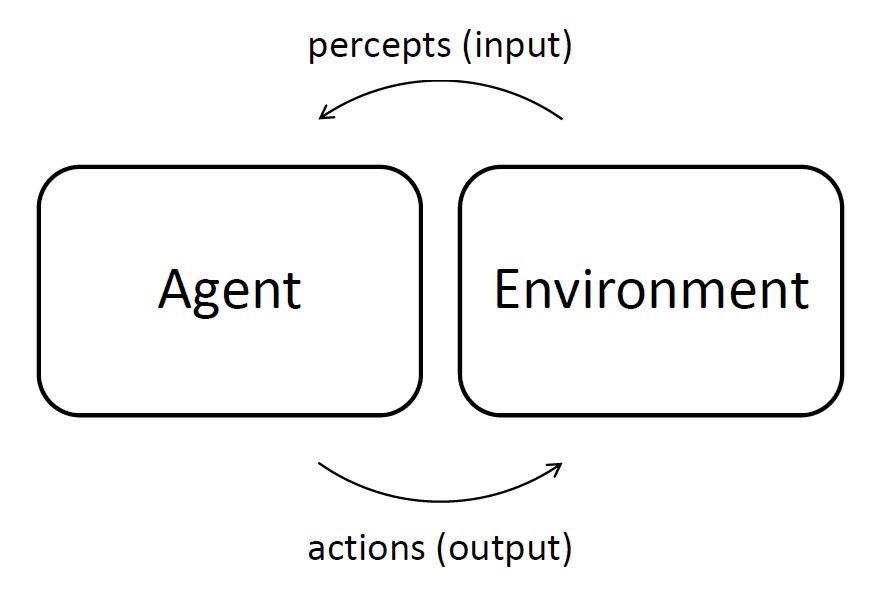
\includegraphics[width=0.4\textwidth]{images/agent-environment-interaction.png}
	\caption{An agent interacting with its environment.}
	\label{figure:agent-environment-interaction}
\end{figure}

% Agent - example: softbot
An example of an agent is a \textit{softbot} (software robot) -- an agent situated in a software environment interacting with it via commands. A softbot's sensors are commands meant to provide information about its environment (e.g. \texttt{ls} or \texttt{pwd} in Unix) and its effectors are commands meant to change the environment (e.g. \texttt{mv} or \texttt{compress} in Unix).

%%%%%%%%%%%%%%%%%%%%%%%%%%%%%%%%%%%%%%%%%%%%%%%%%%%%%%%%%%%%%%%%%%%%%%%%%%%%%%%%
\section{Multi-Agent Systems}

% MAS slogan
There is a popular slogan in the multi-agent systems community: ``There's no such thing as a single agent system'' \cite{Wooldridge09}.

% MAS - definition
\textit{Multi-Agent system}
\footnote{Alternatively spelled multiagent system.}
(MAS) is a system composed of multiple interacting agents.

% MAS vs. single agent
Like a single agent,a MAS is situated in an environment, which means that all its constituent agents are situated in the same environment.
While the single agents field studies agents' interaction with their environment and reasoning about it, the field of MAS deals with agents' interaction with other agents and reasoning about them.
This inter-agent interaction can be either \textit{direct} (via messages) or \textit{indirect} (via environment).

% Empty environment
In this thesis, we do not consider agents' interaction with their environment and we do consider only direct inter-agent interaction -- \textit{communication}.
Hence, we do not assume anything about the environment in which MASs are situated; in fact, as far as the discussion in this thesis goes, MASs do not have to be situated in any environment, i.e. situated in an empty (non-perceivable, non-affectable) environment.

Most importantly, we do not assume any social structure of MASs; a MAS is really just a group of agents with no special relationships among them.
In other words, all agents are equal.
It is the aim of this thesis to introduce social structure to MASs.
%%%%%%%%%%%%%%%%%%%%%%%%%%%%%%%%%%%%%%%%%%%%%%%%%%%%%%%%%%%%%%%%%%%%%%%%%%%%%%%%
%% MASTER'S THESIS                                                            %%
%%                                                                            %% 
%% Title (en): Multi-Agent Systems and Organizations                          %%
%% Title (cs): Multiagentní systémy a organizace                              %%
%%                                                                            %%
%% Author: Bc. Lukáš Kúdela                                                   %%
%% Supervisor: Prof. RNDr. Petr Štěpánek, DrSc.                               %%
%%                                                                            %%
%% Academic year: 2011/2012                                                   %%
%%%%%%%%%%%%%%%%%%%%%%%%%%%%%%%%%%%%%%%%%%%%%%%%%%%%%%%%%%%%%%%%%%%%%%%%%%%%%%%%

\chapter{Organizations in Multi-Agent Systems}

% Quote
\begin{flushright}
\textit{``The achievements of an organization are the results of the combined effort of each individual.''}\\
\textit{--- Vince Lombardi, American football coach}
\end{flushright}

% Chapter intro
In this chapter, we discuss the motivation for introducing organizations to MASs, introduce two conceptions of a MAS and talk about some key organizational concepts for the first time in an informal manner.

% Decomposable problem with independent subproblems
Consider a problem with the following properties:
\begin{itemize}
	\item \textit{decomposability} --- It can easily be decomposed into well-defined subproblems. These subproblems can either be decomposable themselves or atomic.
	Note that the subproblems do not necessarily have to resemble the original problem or each other\footnote{A characteristic necessary for divide and conquer algorithms.}.
	\item \textit{subproblem independence} --- The subproblems can be solved more or less independently and therefore, providing enough computational entities are available, concurrently.
	Note that this is a quantitative characteristic, not a categorical one.
\end{itemize}

% Solving such a problem with a MAS
Such a problem can be solved by first pondering how a society of humans (viewed as intelligent autonomous computational entities) would go about solving it, then modelling this society as a MAS and finally running the system.
However there is an issue we must address---organizational structure of human societies.

% Organizational structure of human societies
In all human societies but the most primitive ones, various types of \textit{organizations}\comments{FO} emerge to facilitate cooperation among their members.
In these organization types \textit{roles}\comments{FO} appear and \textit{interaction protocols}\comments{FO} governing their interaction crystallize among them.
We are facing the challenge of carrying these \textit{organizational concepts} over to the realm of MASs.

% No standardized way to impose organizational structure upon MASs
Unfortunately, there is no standardized way to impose organizational structure upon MASs.
It should come as no surprise to anybody who is familiar with MASs that no single, precise and universally accepted notions of organization, role or interaction protocol currently exist among researchers.
In a plain vanilla MAS, every agent can (in principle) talk to any other agent, regardless of whether this is desirable or even allowed in the society being modelled by the MAS.

% ACMAS vs. OCMAS
In the next two sections, we will introduce two ways of looking at MASs:
\begin{itemize}
	\item \textit{agent-centric}\comments{FO} --- focused on the structure of individual agents (the traditional viewpoint), and
	\item \textit{organization-centric}\comments{FO} --- focused on the structure of agent societies (a novel perspective).
\end{itemize}

%%%%%%%%%%%%%%%%%%%%%%%%%%%%%%%%%%%%%%%%%%%%%%%%%%%%%%%%%%%%%%%%%%%%%%%%%%%%%%%%
\section{Agent-Centric Multi-Agent Systems}

% ACMAS - architecture of individual agents
An \textit{agent-centric multi-agent system} (ACMAS) is the classical conception of a MAS.
It focuses on the architecture of individual agents, being oblivious to the structure of their society.

% ACMAS - characteristics
An ACMAS has the following characteristics \cite{Ferber03}:
\begin{itemize}
	\item Every agent has a public \textit{agent identifier}\footnote{\textit{Agent identifier} (AID) is a name that identifies (that is, labels the identity of) a unique agent.} and it can be addressed with it.
	\item An agent can communicate with any other agent\footnote{Of course, the agent needs to know the other agent's AID, but since these are public, this is not an obstacle.}.
	\item An agent provides a set of services, which are available to every other agent in the system.
	\item It is the responsibility of each agent to constrain its accessibility and the accessibility of its services to other agents.
	\item It is the responsibility of each agent to define its relations, contracts, etc. with other agents.
\end{itemize}

Perhaps ironically, the absolute freedom of interaction in an ACMAS is the cause of many of its shortcomings \cite{Ferber03}:
\begin{itemize}
	\item Predicting the behaviour of the whole system from the behaviour of its constituent components is extremely difficult, if not downright impossible, due to high probability of emergent behaviour.
	\item Because there is no implicit security management, it is easy for a malicious agent to unknowingly misuse or even intentionally abuse the system.
	\item It is not possible to apply the principles of \textit{modular design}. Agents cannot be grouped into modules with different visibilities to the outside world (public vs. private) at design-time, let alone at run-time.
	\item It is not possible to pursue the \textit{framework approach}. There is only one framework---the agent platform itself---and it is impossible to define sub-frameworks with specific interactions.
\end{itemize}

%%%%%%%%%%%%%%%%%%%%%%%%%%%%%%%%%%%%%%%%%%%%%%%%%%%%%%%%%%%%%%%%%%%%%%%%%%%%%%%%
\section{Organization-Centric Multi-Agent Systems}

% OCMAS - structure of agent society (agent social structure)
An \textit{organization-centric multi-agent system} (OCMAS) is the modern conception of a MAS proposed in \cite{Ferber03}.
It focuses on the structure of an agent society, paying no attention to the architecture of the individual agents.

% OCMAS - organizational level vs. agent level
Organizations provide a natural way of describing structure of a MAS and interactions among its constituent agents.
This description is situated on the \textit{organization level}\comments{FO} of an OCMAS---the level above the \textit{agent level}\comments{FO}, which is the only level considered in an ACMAS.
The organizational level contains abstract representations of the concrete organizations occurring on the agent level.

% OCMAS - characteristics
The following are the characteristics of an OCMAS \cite{Ferber03}:
\begin{itemize}
	\item The organizational level imposes social structure and patterns of interaction upon agents, but does not prescribe how agents should behave; it merely demarcates the space within which the agents can express their individuality.
	\item The organizational level does not place constraints on the architecture of the agents; deliberative as well as reactive agents can take part in an organization as longs as they behave in an expected way.
	\item The organizations provide a way to partition a MAS into bounded contexts of interaction.
	Whereas the structure of an organization is known to its members who are able to interact with one another, it is opaque to the non-members whose interaction with the organization (and its members) is limited.
\end{itemize}

\section{Organizational Concepts}

% Organization
An \textit{organization} is a a structured group of agents, which imposes rules on the behaviour and mutual interaction of its members. 
These rules are imposed by roles and interaction protocols defined in the organization.

% Role
A \textit{role} is an interface between an organization and its member; the organization interacts with its members through their roles.
Is is also an interface between the organization members themselves; the members interact with each other via the roles they play.
A role always exists and operates within the context of its defining organization.

% Competence & responsibility
When playing a role, a player is entitled to exercise the role's competences but also obliged to fulfil its responsibilities.
A \textit{competence} is an operation the role's player \textit{can} perform as a result of playing that role.
A \textit{responsibility} is an operation the role's player \textit{has to} perform as a consequence of playing that role.

% Interaction protocol
An \textit{interaction protocol} is a institutionalized pattern of interaction\footnote{In this thesis, the only kind of interaction we consider is communication. Therefore, we will use the terms \textit{interaction} and \textit{communication} interchangeably.} between certain roles in an organization.
It defines by intension a set of possible communication scenarios between the players of these roles.
In the context of a protocol, the participating roles (or their players) are called \textit{parties}.
%%%%%%%%%%%%%%%%%%%%%%%%%%%%%%%%%%%%%%%%%%%%%%%%%%%%%%%%%%%%%%%%%%%%%%%%%%%%%%%%
%% MASTER'S THESIS                                                            %%
%%                                                                            %% 
%% Title (en): Multi-Agent Systems and Organizations                          %%
%% Title (cs): Multiagentní systémy a organizace                              %%
%%                                                                            %%
%% Author: Bc. Lukáš Kúdela                                                   %%
%% Supervisor: Prof. RNDr. Petr Štěpánek, DrSc.                               %%
%%                                                                            %%
%% Academic year: 2011/2012                                                   %%
%%%%%%%%%%%%%%%%%%%%%%%%%%%%%%%%%%%%%%%%%%%%%%%%%%%%%%%%%%%%%%%%%%%%%%%%%%%%%%%%

\chapter{Modelling Organizations---Existing Approaches}

% Chapter intro
In this chapter, we will introduce existing metamodel-based approaches to modelling organizations in MASs.
The initiative to model organizations in MASs using platform-independent metamodels began with the publication of a seminal paper \cite{Ferber98} by Jacques Ferber and Oliver Gutknecht and continues to this day.
We will introduce four metamodels: \textit{Aalaadin}, \textit{O\&P}, \textit{PIM4Agents} and \textit{powerJade}.
All of them have influenced the design of our metamodel to a greater or lesser degree.

% PIM
In software engineering, a \textit{platform-independent model} (PIM) is a model of a software system, that is independent of the specific technological platform used to implement it \cite{Wikipedia-PIM}.
% PIM - motivation
The main motivation to use a PIM is to build the model once and then automatically transform it to any number of platform-specific models for different deployment platforms.

% PSM
The \textit{platform-specific model} (PSM) is a model of a software system, that is bound to a specific technological platform, for example, a hardware environment (processor), operating system or software environment (virtual machine)).
% PSM - motivation
PSMs are indispensable for the actual implementation of a software system \cite{Wikipedia-PSM}

%%%%%%%%%%%%%%%%%%%%%%%%%%%%%%%%%%%%%%%%%%%%%%%%%%%%%%%%%%%%%%%%%%%%%%%%%%%%%%%%
\section{Models and Metamodels}

\subsection{Models and Modelling}

% Models, representation, conformance and modelling
Before talking about metamodels and metamodelling, its absolutely necessary to have a clear understanding of models, modelling and two basic relationships: representation and conformance. 

% Model - representation
A \textit{model} is a simplified \textit{representation} of a certain reality, for example, a system \cite{Genova09}.
A system can be represented by a set of different models.
Each model captures a specific aspect (or view) of the system, depending on the purpose of that particular model.
A model must not represent the system with absolute preciseness; it is useful only because it is a simplified representation \cite{Genova09}.

% Model - conformance
A model also has to be expressed in some modelling language.
Therefore, the full definition of a model is the following: a \textit{model} is a simplified \textit{representation} of a certain reality \textit{conforming} to the rules of a certain modelling language \cite{Genova09}. In short, a model represents a system and conforms to a metamodel. Figure~\ref{figure:representation-and-conformance} illustrates both relationships.

% Figure: Representation and conformance relationships
\begin{figure}[h]
	\centering
	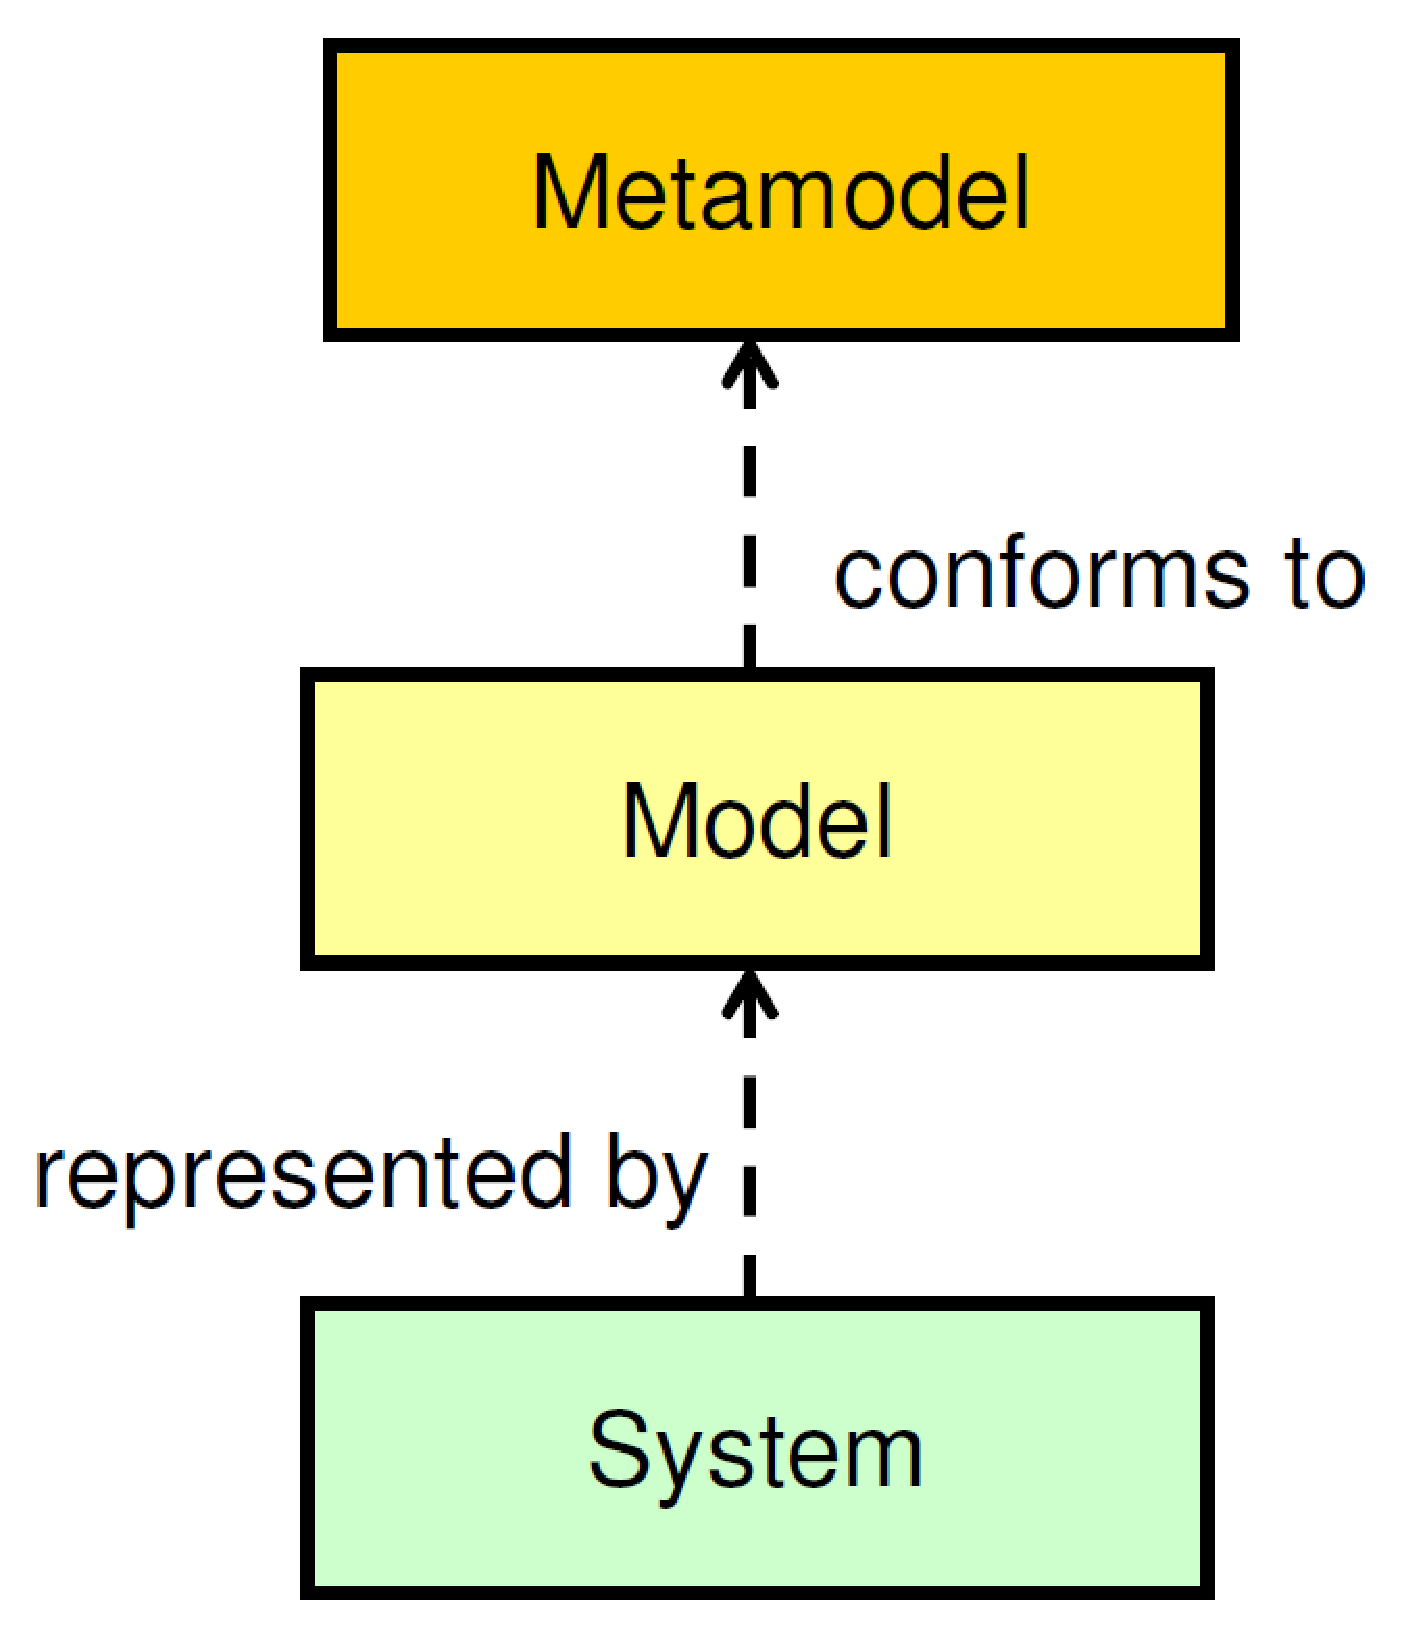
\includegraphics[width=0.3\textwidth]{images/representation-and-conformance-relationships}
	\caption{The representation and conformance relationships \cite{Genova09}}
	\label{figure:representation-and-conformance}
\end{figure}

% Modelling
\textit{Modelling}, in the most general sense, is the use of a model to represent a certain reality for some cognitive purpose.

% Contextual substitutability
A model is characterized by \textit{contextual substitutability}---it should be able to answer a given set of questions in the same way the system would answer them \cite{Genova09}.

\subsection{Metamodels and Metamodelling}

% Metamodel
A \textit{metamodel} is a special kind of model that specifies the abstract syntax of a \textit{modelling language} \cite{OMG-MDA-Foundation-Model}.

% Metamodel - what it represents
A metamodel represents an abstract syntax of a modelling language; it does \textit{not} represent a model or a set of models\footnote{The popular expression ``model of a model'' is particularly confusing.}.
% Metamodel - what it conforms to
A metamodel conforms to a meta-metamodel.

Consider the metalayers shown figure~\ref{figure:metalayers}:

% Figure: Metalayers
\begin{figure}[h]
	\centering
	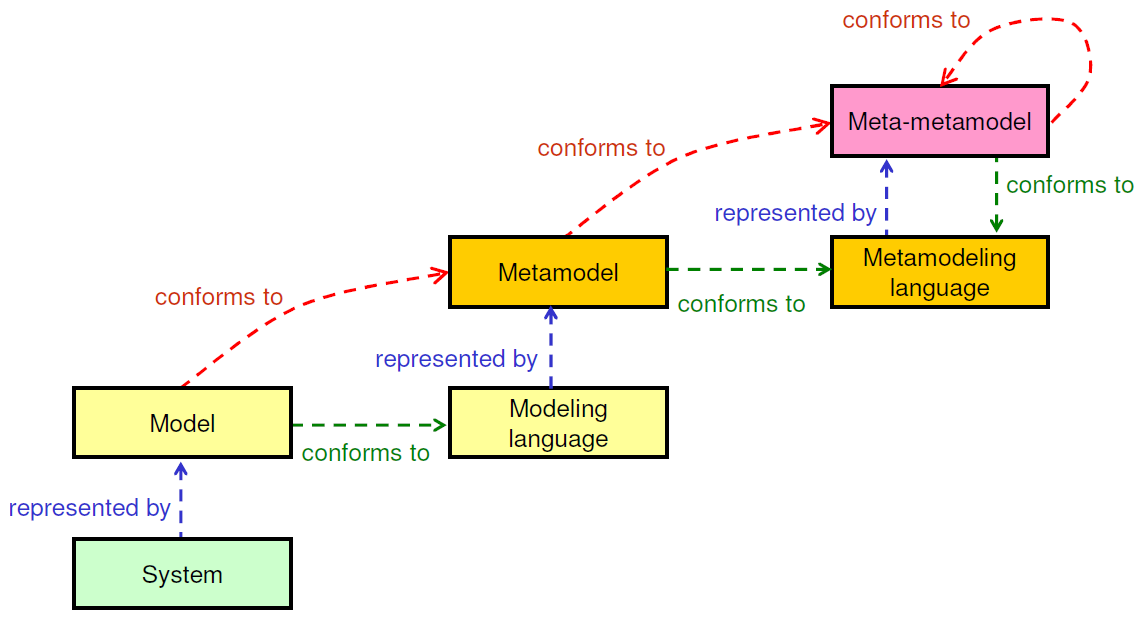
\includegraphics[width=\textwidth]{images/metalayers}
	\caption{Metalayers \cite{Genova09}}
	\label{figure:metalayers}
\end{figure}

% Model conforms to metamodel
On the bottom level, a \textit{model} conforms to a modelling language whose abstract syntax is represented by a \textit{metamodel}.
Transitively, we can say that a \textit{model} conforms to a \textit{metamodel}.

On the middle level, a \textit{metamodel} conforms to a metamodelling language whose abstract syntax is represented by a \textit{meta-metamodel}.
Transitively, we can say that a \textit{metamodel} conforms to a \textit{meta-metamodel}.

On the top level, A \textit{reflexive meta-metamodel} conforms to a language whose abstract syntax is represented by \textit{itself}.
Transitively, we can say that a \textit{meta-metamodel} conforms to \textit{itself}.

% represented-by =/= conforms-to
The represented-by and conforms-to relationships are essentially different; arranging them in the same direction might be confusing.

% Using 'model' to refer to a metamodel
Since metamodels are models themselves, we will use the less cumbersome term---\textit{model}---to refer to a metamodel where it is obvious from the context that we are talking about the metamodel and not one of the models it specifies.  

%%%%%%%%%%%%%%%%%%%%%%%%%%%%%%%%%%%%%%%%%%%%%%%%%%%%%%%%%%%%%%%%%%%%%%%%%%%%%%%%
%% MASTER'S THESIS                                                            %%
%%                                                                            %% 
%% Title (en): Multi-Agent Systems and Organizations                          %%
%% Title (cs): Multiagentní systémy a organizace                              %%
%%                                                                            %%
%% Author: Bc. Lukáš Kúdela                                                   %%
%% Supervisor: Prof. RNDr. Petr Štěpánek, DrSc.                               %%
%%                                                                            %%
%% Academic year: 2011/2012                                                   %%
%%%%%%%%%%%%%%%%%%%%%%%%%%%%%%%%%%%%%%%%%%%%%%%%%%%%%%%%%%%%%%%%%%%%%%%%%%%%%%%%

\section{Aalaadin}

% Aallaadin - authors
This section introduces the \textit{Aalaadin} metamodel\footnote{\textit{Aalaadin} is the old name; the metamodel is now known as \textit{AGR} (for ``Agent, Group and Role''). We will use the fancier old name.} \cite{Ferber97}, \cite{Ferber98}, \cite{Ferber00} and \cite{Ferber03}, proposed in 1997 by Jacques Ferber, Oliver Gutknecht and their colleagues from Montpellier 2 University in Montpellier, France.
% Citation
The overview presented here is distilled from the seminal paper on \textit{Aalaadin} \cite{Ferber97}.

%% Aalaadin %%%%%%%%%%%%%%%%%%%%%%%%%%%%%%%%%%%%%%%%%%%%%%%%%%%%%%%%%%%%%%%%%%%%%

% Abstract organization vs. concrete organization
To understand the following text, it is essential to make a distinction between an \textit{abstract organization}\comments{FO} and a \textit{concrete organization}\comments{FO}.
An \textit{abstract organization} is the organization specification that exists in a MAS at design-time, whereas a \textit{concrete organization} is the actual organization that exists in a MAS at run-time.
Put differently, an abstract organization is a (possibly infinite) set of all imaginable organizations conforming to a common specification (sharing the same role structure) and a concrete organization is a member of this set.

% Organization type vs. organization token
Later we will use the terms \textit{organization type} and \textit{organization token} to refer to an abstract organization and a concrete organization respectively.
These terms try to capture the essence of the relationship between an abstract and concrete organization (namely, a concrete organization being an instance of an abstract organization and conversely, an abstract organization being a class of a concrete organization)

% Two models: concrete and abstract
The \textit{Aalaadin} metamodel comprises two models: \textit{Core model} and \textit{Methodological model}.

%%%%%%%%%%%%%%%%%%%%%%%%%%%%%%%%%%%%%%%%%%%%%%%%%%%%%%%%%%%%%%%%%%%%%%%%%%%%%%%%
\subsection{Core Model}

% Core model - about
The \textit{Core model} contains concepts for modelling concrete organizations, the so-called \textit{core} concepts: \textit{Agent}, \textit{Group} and \textit{Role}.
Figure~\ref{figure:aalaadin-core-model} illustrates the \textit{Core model}.

% Figure: Core model
\begin{figure}[h]
	\centering
	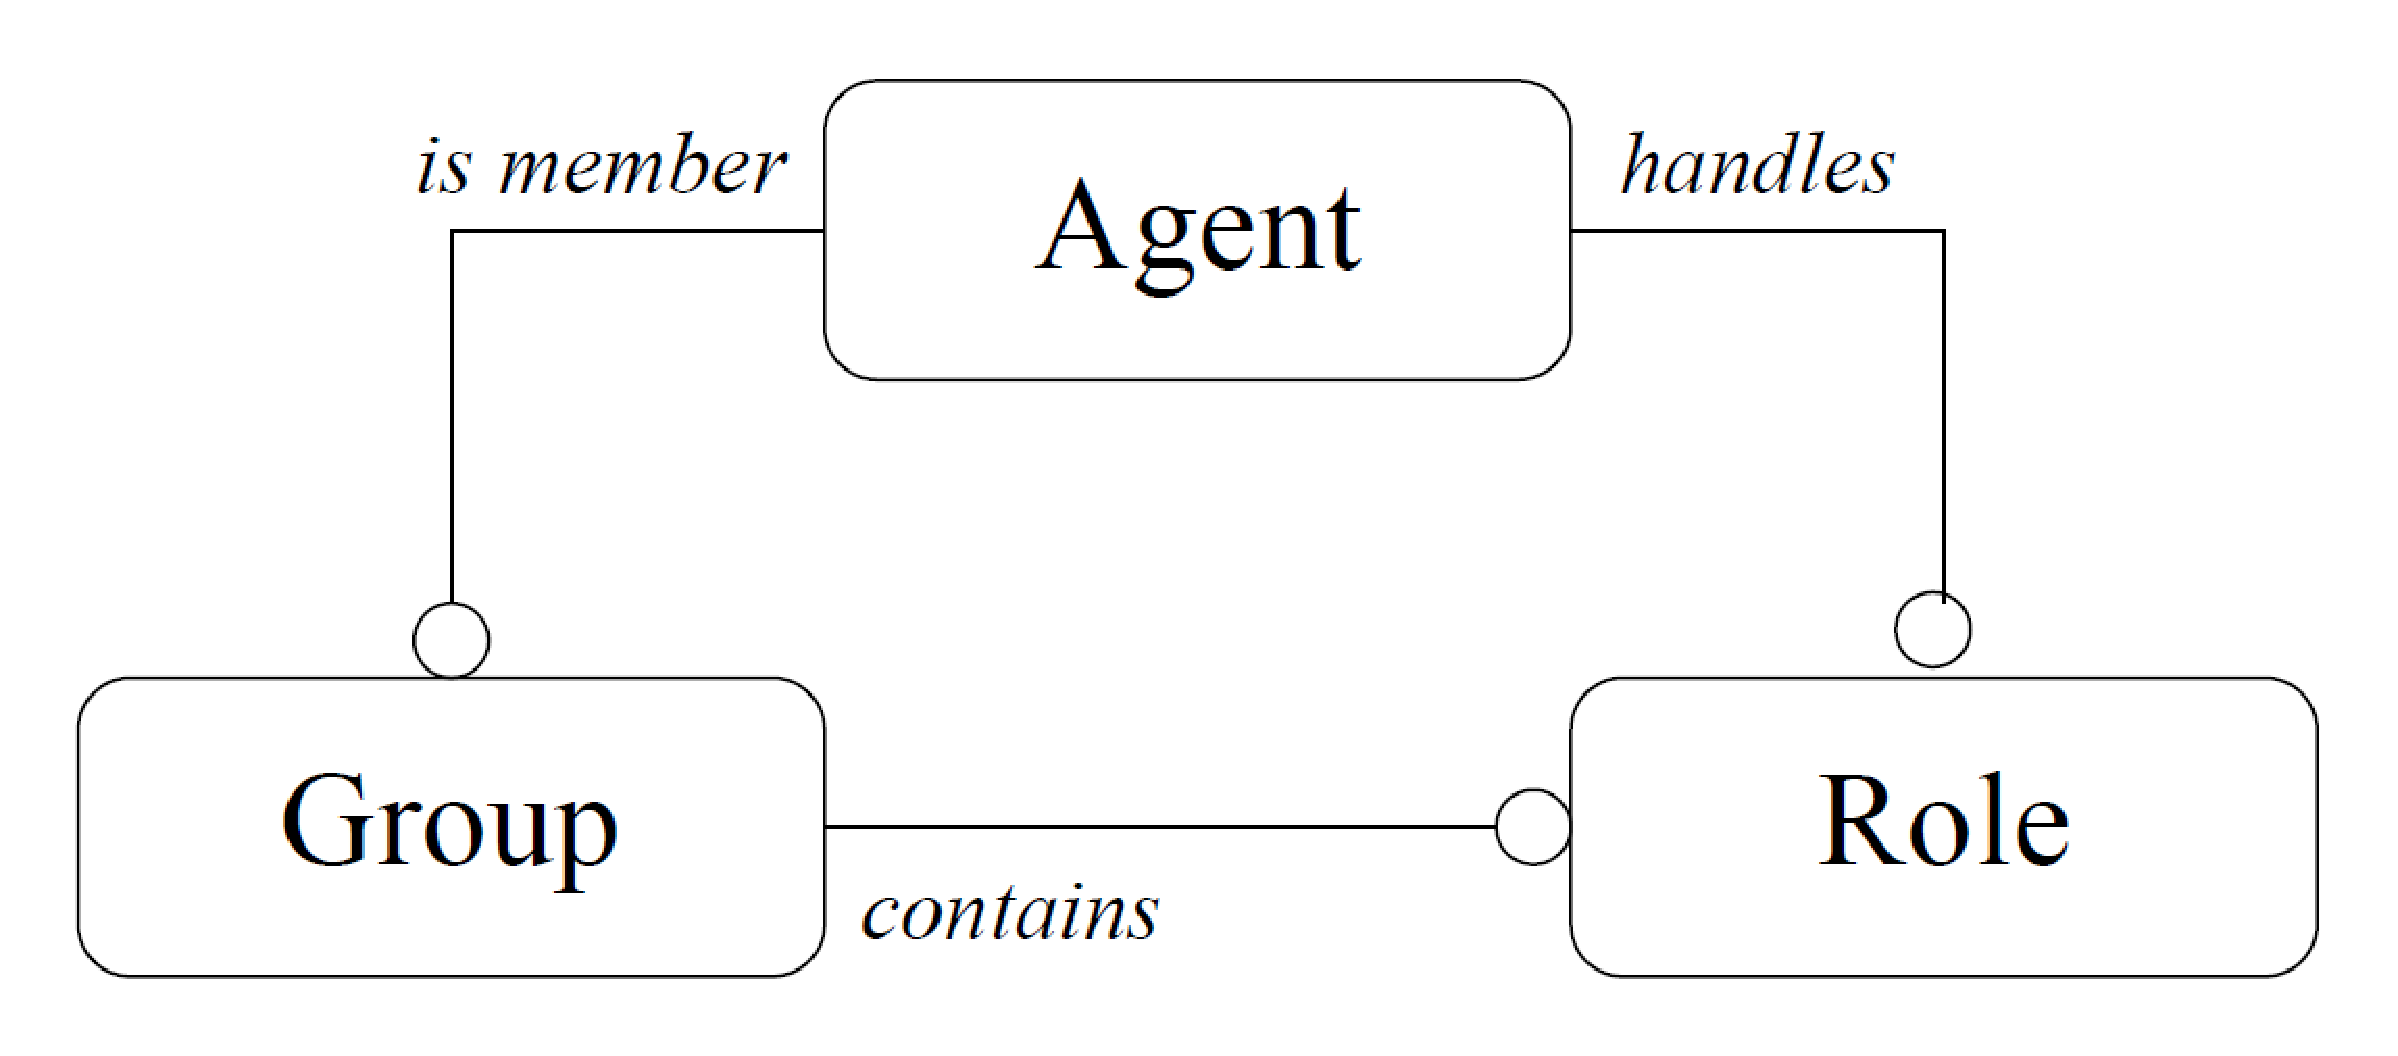
\includegraphics[width=0.4\textwidth]{images/aalaadin/core-model}
	\caption{The \textit{Core model} \cite{Ferber97}}
	\label{figure:aalaadin-core-model}
\end{figure}

\subsubsection*{Agent}

% Agent - definition
An \textit{agent} is defined in \cite{Ferber97} as an active communicating entity which plays roles within groups.

% Agent - no agent architecture imposed
\textit{Aalaadin} does not prescribe any particular agent architecture.
Indeed, any MAS metamodel striving for generality should impose as few constraints upon the resulting MAS models as possible.
After all, the decision of which agent architecture to employ is best made by the the MAS designer and relates to the MAS as such, not just its organizational structure.
As we will see, none of the metamodels introduced in this thesis force the MAS designer to adapt a concrete definition of agenthood.

\subsubsection*{Group}

% Group - definition
In \cite{Ferber97}, a \textit{group} is defined as atomic set of agent aggregation.
In its most basic form, a group is just a way to tag a set of agents, i.e. it has no structure.

% Group - characteristics
Groups have the following characteristics:
\begin{itemize}
	\item An agent can be a member of a number of groups simultaneously.
	This means that groups can overlap, which is major point of \textit{Aalaadin}.
	\item A new group can be founded by any agent; an agent must request its admission to an existing group.
	\item A group may be local or distributed across multiple machines.
\end{itemize}

The real advantage of grouping agents becomes apparent when we use roles to impose some structure to these groups.

\subsubsection*{Role}

% Role - definition
A \textit{role} is an abstract representation of an agent function, service or identification within a group \cite{Ferber97}.
An agent can play multiple roles, each of which is local to a particular group.
Similarly to group admission, playing a role in a group must be requested by the candidate agent (already a member of the group) and awarded by the group founder agent.

% Role & communication
In \textit{Aalaadin}, the communication is related to roles. Since an agent can play multiple roles, it can be engage in several independent dialogues simultaneously.

% Role - definition characteristics
The following characteristics are part of a role definition:
\begin{itemize}
	\item a \textit{uniqueness characteristic}---an indication whether the role is \textit{single} or \textit{multiple},
	\item a list of  \textit{competences}---conditions the candidate agent must satisfy to be eligible to play the role, and
	\item a list of \textit{capacities}---abilities attributed to an agent while it is playing the role.
\end{itemize}
A \textit{single role} can be played by at most one agent in a group, whereas a \textit{multiple role} can be played by any number of agents within a group.
By default a role is multiple, does not require any competences and does not provide any capacities.

% Group manager role
A special role in a group is the \textit{group manager} role, which is automatically granted to the group founder.
It has a competence to handle group membership and role playing requests.
It also has a capacity to revoke roles and cancel group membership.

%%%%%%%%%%%%%%%%%%%%%%%%%%%%%%%%%%%%%%%%%%%%%%%%%%%%%%%%%%%%%%%%%%%%%%%%%%%%%%%%
\subsection{Methodological Model}

% Methodological model - about
The \textit{Methodological model} contains concepts for modelling abstract organizations, the so-called \textit{methodological} concepts: \textit{Organization structure}, \textit{Group structure}, \textit{Interaction} and \textit{Agent class}.
These concepts are not present directly in concrete organizations, but only serve during the analysis and design phases.
Their purpose is to describe abstract organizations from which concrete organizations, described using the core concepts, will ultimately be derived.
Figure~\ref{figure:aalaadin-metamodel} shows the integrated \textit{Aalaadin} metamodel. The dotted ellipsis is the demarcation line between the \textit{Core model} and \textit{Methodological model}.

% Figure: Aalaadin metamodel
\begin{figure}[h]
	\centering
	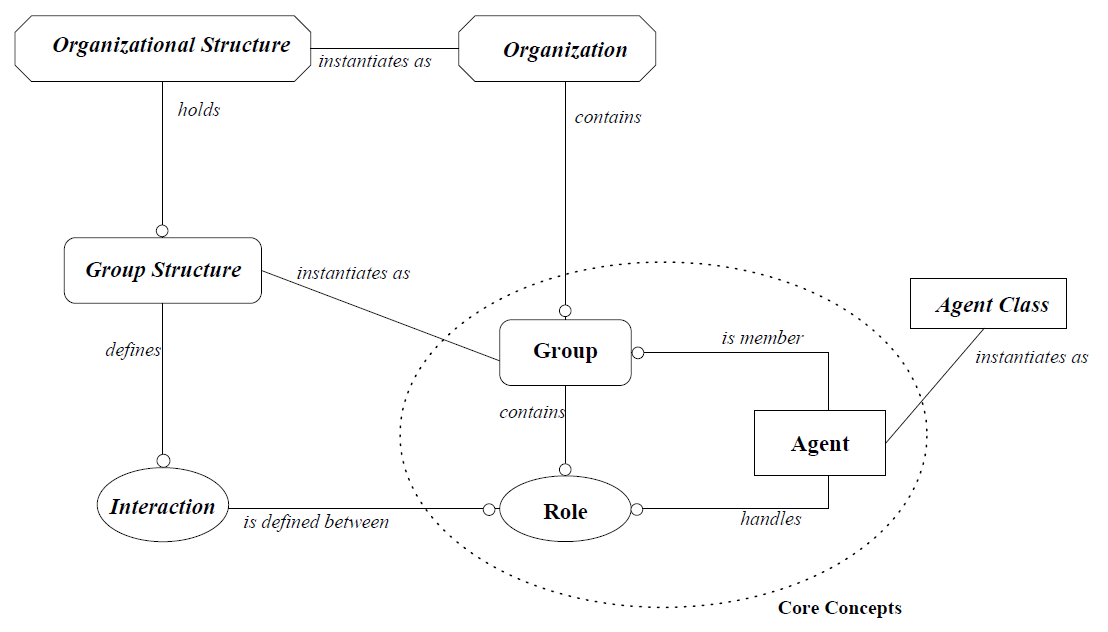
\includegraphics[width=\textwidth]{images/aalaadin/aalaadin-metamodel}
	\caption{The \textit{Aalaadin} metamodel \cite{Ferber97}}
	\label{figure:aalaadin-metamodel}
\end{figure}

\subsubsection*{Group Structure}

% Group structure - definition
A \textit{group structure} is an abstract description of a group \cite{Ferber97}.
It identifies all roles comprising the group and defines interactions among them.

% Group structure - definition characteristics
A group structure is defined by
\begin{itemize}
	\item a set of available roles that can be played by agents in the group, and
	\item a set of valid interaction schemes between the roles.
\end{itemize}

% Group structure - partial instantiation
Note that an actual group might be a partial instantiation of its defining group structure.
This means that during the MAS run, there might be a moment when some roles defined in the group structure are not played in an actual group.
This dynamic nature of groups allows for a great deal of run-time flexibility.

\subsubsection*{Organizational Structure}

% Organizational structure - definition
The \textit{organizational structure}, as defined in \cite{Ferber97}, is a set of group structures expressing the design of a multi-agent organization scheme.

% Organizational structure - about
The organizational structure can be seen as the specification of the problem to be solved (organization to be modelled) using a MAS.
Any sort of heterogeneity within a single system (e.g. agent architecture heterogeneity or language heterogeneity) can be managed by different group structures involved in the organizational structure.

% Organizational structure - partial instantiation
Similarly to groups, an asctual organization can be a incomplete manifestation of its defining organizational structure.
This means that while a MAS is running, there may be a point when some groups defined in the organizational structure are not present in an organization.
This also contributes to the overall run-time flexibility.

%%%%%%%%%%%%%%%%%%%%%%%%%%%%%%%%%%%%%%%%%%%%%%%%%%%%%%%%%%%%%%%%%%%%%%%%%%%%%%%%
\subsection{MadKit}

% MadKit - authors & references
The authors of \textit{Aalaadin} also developed an agent platform implementing their metamodel called \textit{MadKit}\footnote{Multi-Agent Development Kit ---\url{http://www.madkit.org/}} \cite{Ferber97}, \cite{Ferber98} and \cite{Gutknecht00}.

% MadKit - basic philosophy
The basic philosophy of the \textit{Aalaadin/MadKit} architecture is to use the platform itself for its own management wherever possible.
\textit{MadKit's} main design principles are \textit{micro-kernel architecture} and \textit{agentification of services}---all services except for the most fundamental ones provided by the micro-kernel are implemented as agents, organized in groups and identified by roles \cite{Ferber98}.

%%%%%%%%%%%%%%%%%%%%%%%%%%%%%%%%%%%%%%%%%%%%%%%%%%%%%%%%%%%%%%%%%%%%%%%%%%%%%%%%
%% MASTER'S THESIS                                                            %%
%%                                                                            %% 
%% Title (en): Multi-Agent Systems and Organizations                          %%
%% Title (cs): Multiagentní systémy a organizace                              %%
%%                                                                            %%
%% Author: Bc. Lukáš Kúdela                                                   %%
%% Supervisor: Prof. RNDr. Petr Štěpánek, DrSc.                               %%
%%                                                                            %%
%% Academic year: 2011/2012                                                   %%
%%%%%%%%%%%%%%%%%%%%%%%%%%%%%%%%%%%%%%%%%%%%%%%%%%%%%%%%%%%%%%%%%%%%%%%%%%%%%%%%

\section{O\&P}

% O&P - authors
This section introduces the \textit{O\&P} metamodel\footnote{The metamodel was not given a name by its authors. In this thesis, we will call it \textit{O\&P}.} \cite{Odell01}, \cite{Parunak02}, \cite{Odell03b}, \cite{Odell04b} and \cite{Odell05}, put forward in 2001 by James J. Odell, H. van Dyke Parunak and their colleagues.
% Citation
The overview presented here is extracted from the most complete paper on \textit{O\&P} \cite{Odell05}.

%% O&P %%%%%%%%%%%%%%%%%%%%%%%%%%%%%%%%%%%%%%%%%%%%%%%%%%%%%%%%%%%%%%%%%%%%%%%%%

%%%%%%%%%%%%%%%%%%%%%%%%%%%%%%%%%%%%%%%%%%%%%%%%%%%%%%%%%%%%%%%%%%%%%%%%%%%%%%%%
\subsection{Integrated Metamodel}

% Integrated model - about
Figure~\ref{figure:onp-metamodel} shows the integrated metamodel proposed in \cite{Odell05}.
The following subsections will focus on parts of the integrated metamodel that can be studied in isolation.
We present the full metamodel before discussing its parts so that the reader can follow the discussion knowing how each part fits into the big picture.

% Figure: O&P metmodel
\begin{figure}[ht]
	\centering
	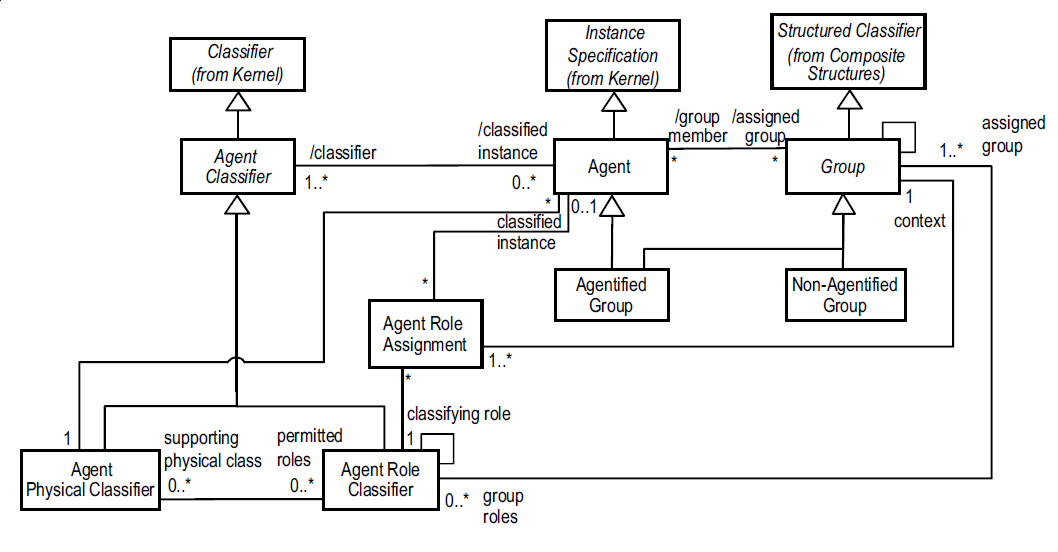
\includegraphics[width=\textwidth]{images/onp/onp-metamodel.png}
	\caption{The integrated \textit{O\&P} metamodel \cite{Odell05}}
	\label{figure:onp-metamodel}
\end{figure}

% UML Classifier vs. UML Class
To understand the integrated metamodel, it is essential to differentiate between the \textit{Classifier} and \textit{Class} UML classes.
In short, \textit{Classifier} does not have the features associated with a OOP class (e.g. the extended class, the list of implemented interfaces or attributes), while \textit{Class}, obviously, has them.
\textit{Class} is in fact a specialization of \textit{Classifier}.
It is important to make this distinction, because the agent classification is based on an extension of \textit{Classifier}, not \textit{Class}.
The reason for this is that the authors did not want to impose object-orientation upon their metamodel.
After all, it is not at all expected of an agent to exhibit behaviour intrinsic to an object, such as polymorphism.

%%%%%%%%%%%%%%%%%%%%%%%%%%%%%%%%%%%%%%%%%%%%%%%%%%%%%%%%%%%%%%%%%%%%%%%%%%%%%%%%
\subsection{Agent Classifiers and Agent Model}

\subsubsection*{Agent Classifier}

\textit{Agent Classifier} is a UML \textit{Classifier} that specifically provides a way to classify agent instances by a set of features that they have in common \cite{Odell05}.
Classification is important because it enables a common definition of a set of entities that are in some sense similar, i.e. share some features and/or capabilities.

Figure~\ref{figure:onp-agent-classifiers} shows \textit{Agent Classifier} and its two specializations: \textit{Agent Physical Classifier} and \textit{Agent Role Classifer}.

\begin{figure}[ht]
	\centering
	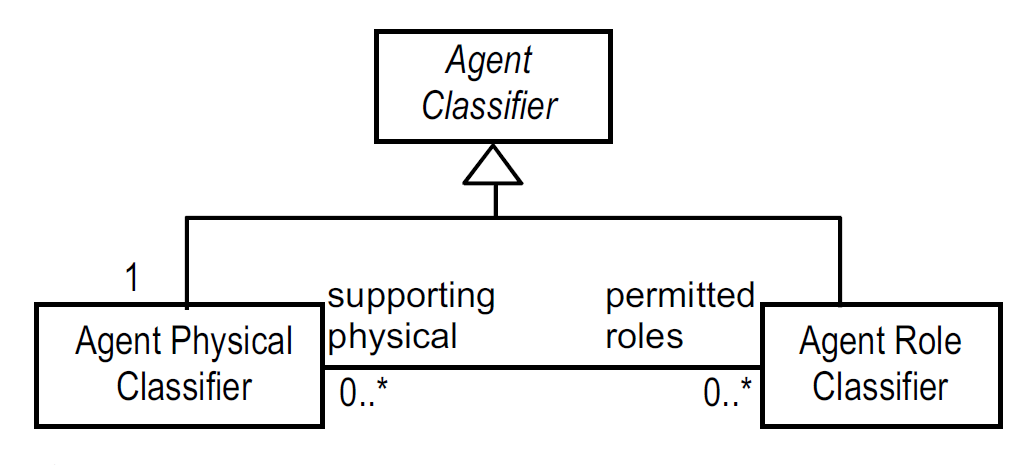
\includegraphics[width=0.6\textwidth]{images/onp/agent-classifiers.png}
	\caption{\textit{Agent Classifier} and its two specializations: \textit{Agent Physical Classifier} and \textit{Agent Role Classifier} \cite{Odell05}}
	\label{figure:onp-agent-classifiers}
\end{figure}

\subsubsection*{Agent Physical Classifier}

% Physical classifier - definition
The purpose of \textit{Agent Physical Classifier} is to define a set of features that an agent classified with it has independent of roles it plays \cite{Odell05}.
Every agent must be classified with exactly one physical classifier\footnote{Compare this with OOP, where every object must be an instance of exactly one class.} and is never reclassified during its lifetime.

% Physical classifiers vs. role classifiers
In contract to role classifiers, physical classifiers attribute primary and permanent features to agents.
Examples of physical classifiers from the real world are \textit{Human}, \textit{Male} or \textit{Female}.

Figure~\ref{figure:onp-physical-classifier-examples} shows some examples of physical classifiers forming a small class hierarchy.
Notice the \stereotype{agent physical classification} stereotype.

% Figure: Physical classifer examples
\begin{figure}[ht]
	\centering
	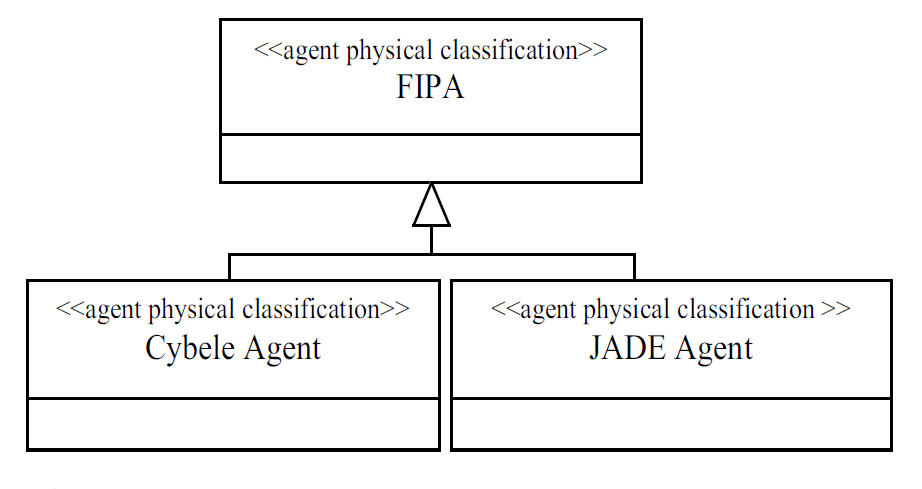
\includegraphics[width=0.5\textwidth]{images/onp/physical-classifier-examples.png}
	\caption{Examples of physical classifiers forming a class hierarchy \cite{Odell05}}
	\label{figure:onp-physical-classifier-examples}
\end{figure}

\subsubsection*{Agent Role Classifier}

% Role classifier - definition
\textit{Agent Role Classifier} is a classifier that defines a set of features that an agent classified with it acquires.
An agent can be classified with more than one role classifier at once (\textit{multiple classification}) and can be reclassified over time (\textit{dynamic classification}).

In comparison to physical classifiers, role classifiers ascribe secondary and transient features to agents.
An example of a role classifier from the real world would be \textit{Chess player}.

% Role hierarchy vs. class hierarchy
Figure~\ref{figure:onp-role-classifier-examples} depicts a small class hierarchy of role classifiers.
Notice the \stereotype{agent role} stereotype.

% Figure: Role classifer examples
\begin{figure}[ht]
	\centering
	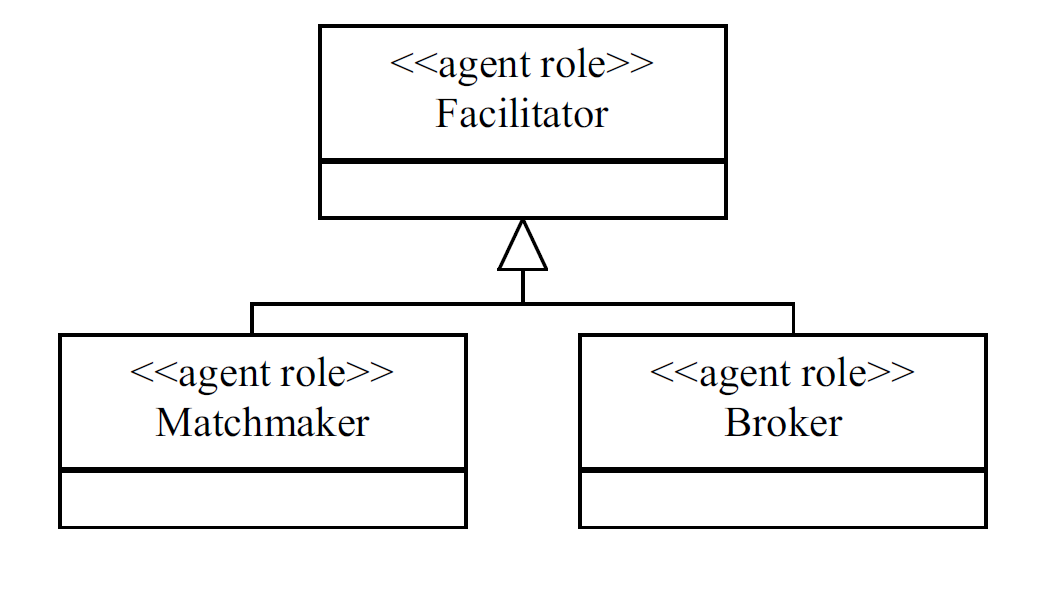
\includegraphics[width=0.5\textwidth]{images/onp/role-classifier-examples.png}
	\caption{Examples of role classifiers forming a class hierarchy \cite{Odell05}}
	\label{figure:onp-role-classifier-examples}
\end{figure}

\subsubsection*{Agent}

In \textit{O\&P}, the basic concepts are \textit{Agent Classifier} and \textit{Agent}.
These modelling constructs are considered fundamental, because they enable a MAS designer to model agents classes and agent instances respectively.
Agent classes are the design-time constructs providing the classification of the run-time constructs---agent instances.

\subsubsection*{Association between Agent Physical Classifier and Agent Role Classifier}

The association between \textit{Agent Physical Classifier} and \textit{Agent Role Classifier} specifies which role classifiers are permitted for each physical classifier, independent of the capabilities of the individual agents classified with that particular physical classifier \cite{Odell05}.

Figure~\ref{figure:onp-physical-classifier-role-classifier-association} illustrates this association.
It can be interpreted as follows. \textit{Jade} agents can play the \texttt{Broker} and \texttt{Manager} roles, and \textit{Cybele} agents can take on the role of \texttt{Broker}, \texttt{Trust Manager} and \texttt{Buyer}.

% Figure: Agent physical classifier <---> Agent role classifier association
\begin{figure}[ht]
	\centering
	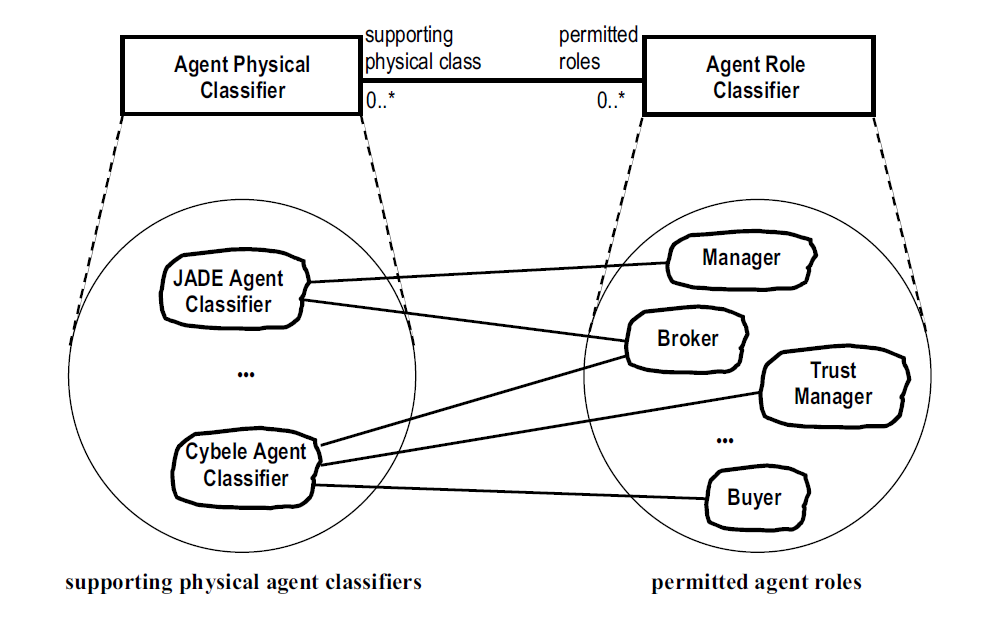
\includegraphics[width=0.8\textwidth]{images/onp/physical-classifier-role-classifier-association.png}
	\caption{The association between \textit{Agent Physical Classifier} and \textit{Agent Role Classifier} \cite{Odell05}}
	\label{figure:onp-physical-classifier-role-classifier-association}
\end{figure}

\subsubsection*{Association between Agent and Agent Classifier}

The association between \textit{Agent} and \textit{Agent Classifier} defines agents' features.
Each agent classifier classifies an agent as a member of a set of agents sharing some physical or role-related features.

% Physical vs. role classification
There are two main differences between the physical and role classification. First, the role classification is \textit{multiple} whereas the physical classification is \textit{single}.
While an agent can be classified with more than one (or even none) role classifiers at the same time, it must be classified with exactly one physical classifiers.
Second, the role classification is \textit{dynamic} in contrast to physical classification, which is \textit{static}.
Dynamic classification means that an agent can be declassified or reclassified with another role after the initial classification; static classification is invariant in time.

Figure~\ref{figure:onp-agent-agent-classifier-association} illuminates this association.
It can be read as follows. \texttt{Agent1}, a \textit{Jade} agent, is a \texttt{Manager}; \texttt{Agent2}, a \textit{Cybele} agent, is a \texttt{Manager} and \texttt{Buyer}; \texttt{Agent3}, another \textit{Cybele} agent, is a \texttt{Trust Manager}; and \texttt{Agent4}, also a \textit{Cybele} agent, is a \texttt{Broker}.

% Figure: Agent <---> Agent Classifier association
\begin{figure}[ht]
	\centering
	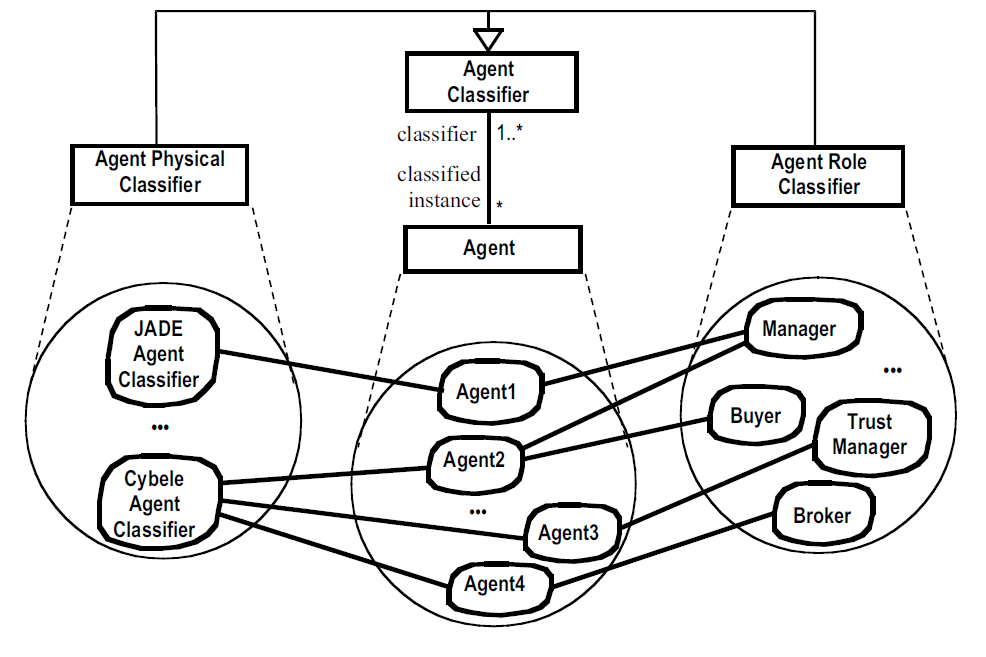
\includegraphics[width=0.8\textwidth]{images/onp/agent-agent-classifier-association.png}
	\caption{The association between \textit{Agent} and \textit{Agent Classifiers} \cite{Odell05}}
	\label{figure:onp-agent-agent-classifier-association}
\end{figure}

%%%%%%%%%%%%%%%%%%%%%%%%%%%%%%%%%%%%%%%%%%%%%%%%%%%%%%%%%%%%%%%%%%%%%%%%%%%%%%%%
\subsection{Group Model}

\subsubsection*{Group}

% Group - definition
A \textit{group} is a set of agents that are related via their roles, where these links must form
a connected graph within the group \cite{Odell05}.
This is the agent-centric way of lookig at a group.
Another way of to look at it is the role-centric way: a group is a composite structure consisting of interrelated roles, where each of the group's roles has a number of agent instances \cite{Odell05} playing that role.
A group can be formed to exploit the synergy of its members, resulting in an entity capable of performing operations that none of its constituents alone is capable of performing on its own.

Figure~\ref{figure:onp-group} shows the \textit{Group} class and its associations with \textit{Agent} and \textit{Role}.
The abstract \textit{Group} class extends the UML \textit{Structured Classifier}, which means that \textit{Group} is defined as composite structure\footnote{In UML, \textit{Structured Classifier} can be thought of as a structured set of classifiers. From this perspective, \textit{Group} is a structured set of \textit{Agent Role Classifiers}.}.

% Figure: Group
\begin{figure}[ht]
	\centering
	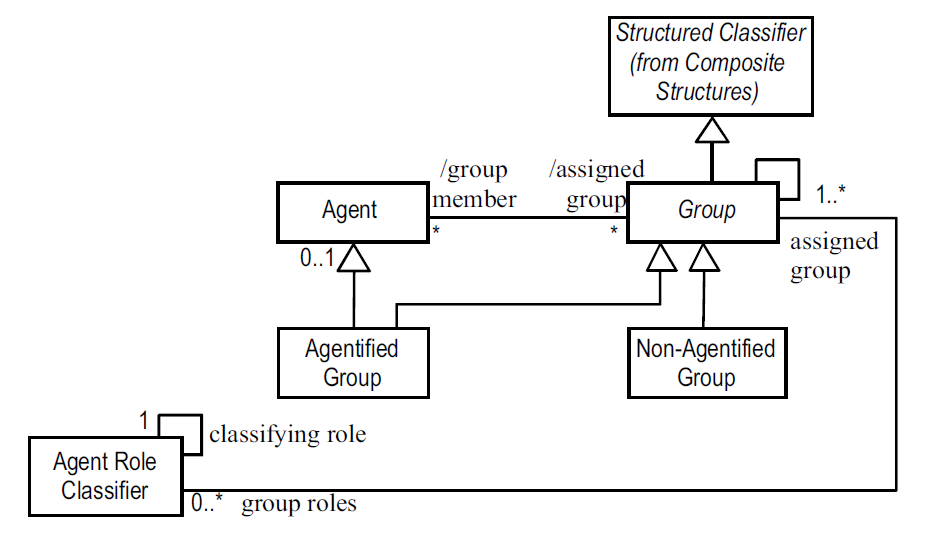
\includegraphics[width=0.8\textwidth]{images/onp/group.png}
	\caption{The \textit{Group} class and its associations \cite{Odell05}}
	\label{figure:onp-group}
\end{figure}

\subsubsection*{Association between Group and Agent}

% Association between Group and Agent
Conceptually, a group is constituted by a set of agents playing roles within that group.
The roles that the agents can play are represented by one or more agent role classifiers associated with this group.
Therefore, the set of agents forming a group can be derived from the group via the agent role classifiers \cite{Odell05}.

\subsubsection*{Association between Group and Role}

% Association between Group and Agent Role Classifier
Figure~\ref{figure:onp-group-role-association} illustrates the association between \textit{Group} and \textit{Role}.
Note that groups containing no roles are not allowed; each group must contain at least one role.
Also observe that each role has to be defined in at least one group, since roles only make sense within the context of a group.

% Figure: Group <---> Role association
\begin{figure}[ht]
	\centering
	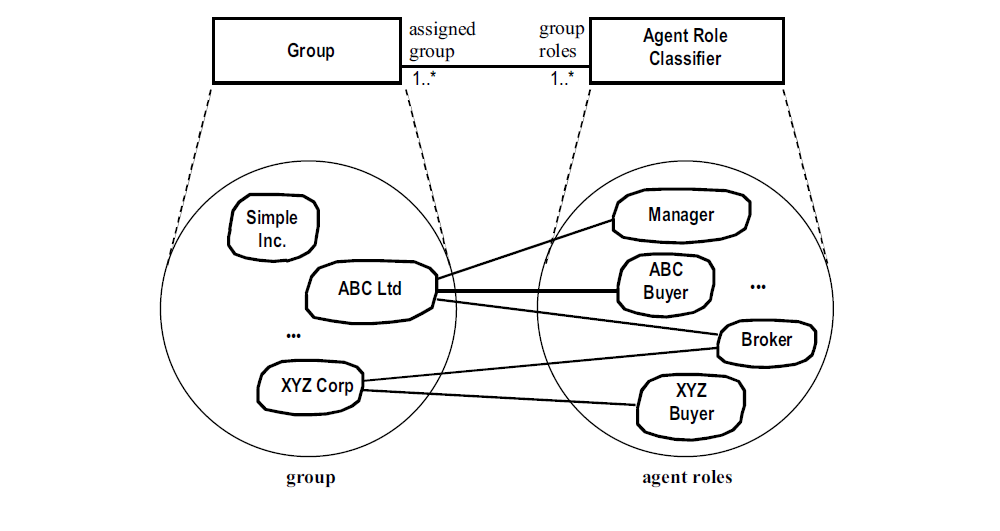
\includegraphics[width=0.8\textwidth]{images/onp/group-role-association.png}
	\caption{The association between \textit{Group} and \textit{Role} \cite{Odell05}}
	\label{figure:onp-group-role-association}
\end{figure}

\subsubsection*{Agentified and Non-Agentified Groups}

\textit{O\&P} differentiates between two types of groups: \textit{agentified}\comments{FO} and \textit{non-agentified}\comments{FO}.

% Agentified group
An \textit{agentified group} is a group that is also an agent in its own right, which means it has its own capability to interact \cite{Odell05}.
An agentified group can communicate with other agents (or agentified groups) directly, i.e. without a representative agent.
It can also be a member of other groups (agentified or not) and play roles like any other agent.
To achieve this in \textit{O\&P}, \textit{Agentified Group} is a subclass of both the \textit{Group} and \textit{Agent} classes.
Figure~\ref{figure:onp-agentified-group} shows an example of an agentified group.
Notice the \stereotype{agent} stereotype used to mark the group as agentified.

% Figure: agentified group
\begin{figure}[ht]
	\centering
	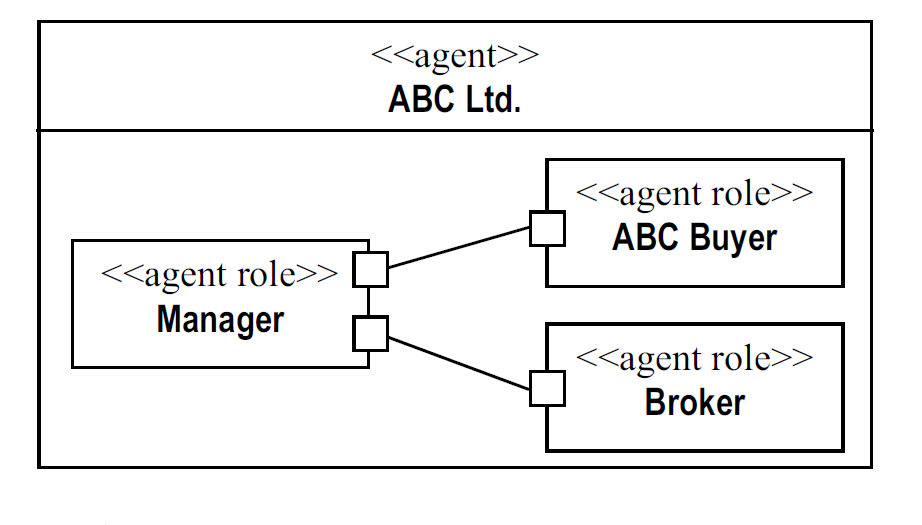
\includegraphics[width=0.5\textwidth]{images/onp/agentified-group.png}
	\caption{An example of an agentified group \cite{Odell05}}
	\label{figure:onp-agentified-group}
\end{figure}

% Non-agentified group
A \textit{non-agentified group}, while still being a first-class citizen, is not an agent in and of itself, meaning it has no capability to interact of its own.
A non-agentified group always communicates with other agents (including agentified groups) through one of its members acting as an intermediary.
This is achieved in \textit{O\&P} by \textit{Non-Agentified Group} subclassing only the \textit{Group} class and not the \textit{Agent} class.
An example of a non-agentified group is shown in figure~\ref{figure:onp-non-agentified-group}.
Notice the absence of the \stereotype{agent} stereotype.

% Figure: non-agentified group
\begin{figure}[ht]
	\centering
	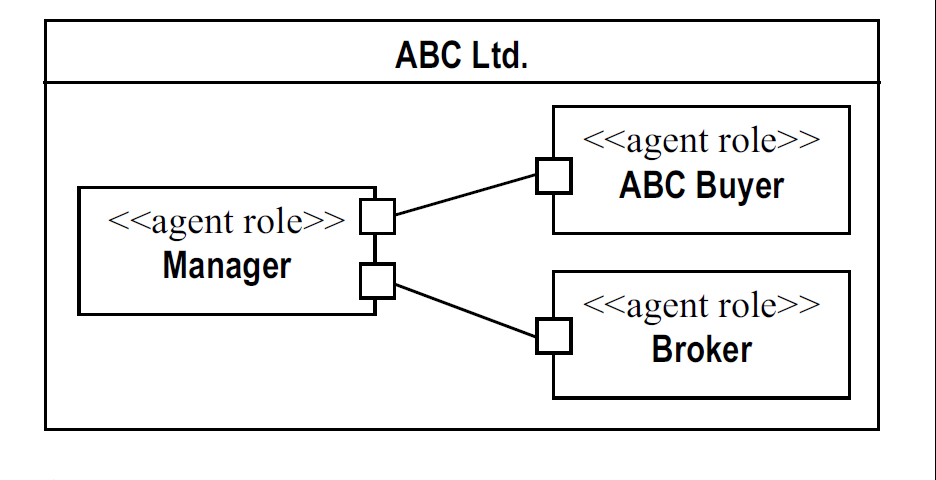
\includegraphics[width=0.5\textwidth]{images/onp/non-agentified-group.png}
	\caption{An example of a non-agentified group \cite{Odell05}}
	\label{figure:onp-non-agentified-group}
\end{figure}

%%%%%%%%%%%%%%%%%%%%%%%%%%%%%%%%%%%%%%%%%%%%%%%%%%%%%%%%%%%%%%%%%%%%%%%%%%%%%%%%
\subsection{Agent Role Assignment}

The assignment of roles to agents is dynamic, i.e. it changes in time, and is modelled by \textit{Agent Role Assignment}.
Figure~\ref{figure:onp-agent-role-assignment} shows the \textit{Agent Role Assignment} class and its associations.

% Figure: Agent Role Assignment class
\begin{figure}[ht]
	\centering
	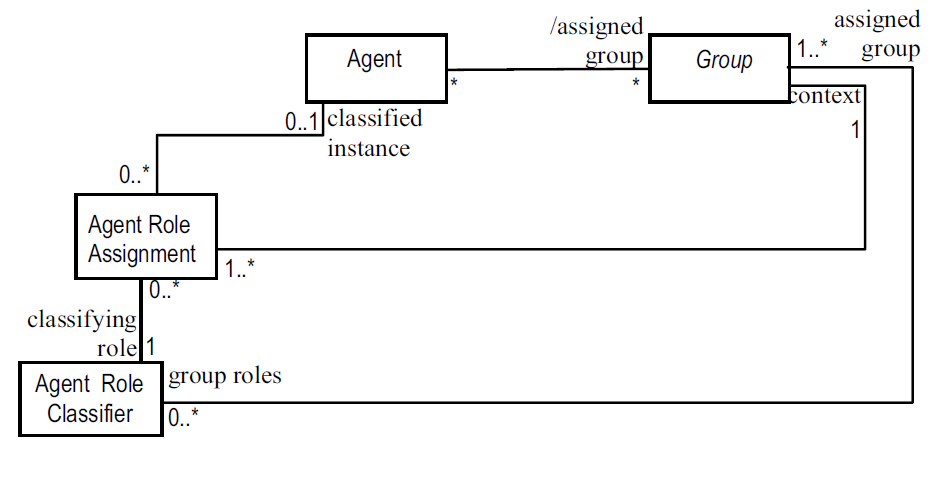
\includegraphics[width=0.8\textwidth]{images/onp/agent-role-assignment.png}
	\caption{The \textit{Agent Role Assignment} class and its associations \cite{Odell05}}
	\label{figure:onp-agent-role-assignment}
\end{figure}

\subsubsection*{Agent Role Assignment as a Ternary Association}

A model with a direct association between \textit{Agent} and \textit{Agent Role Classifier} could represent agents playing roles.
However, such model would not be able to represent a situation where an agent plays a role in one group but does not play it in another.
To model this kind of situation, it is necessary to augment the agent-to-role association with a group context.
This yields a ternary association, reified\footnote{\textit{Reification} is the process of turning an implicit abstract idea about some concept into an explicit concrete model of that concept.} in \textit{O\&P} as the \textit{Agent Role Assignment} class, whose instances link an agent to a role in a group.

\subsubsection*{Position}

It is possible to associate a group with a role leaving an agent unspecified.
Such association is called a \textit{position} and represents a situation where a concrete agent playing a role within a particular group is yet to be determined.
This turns out to be an extremely useful modelling concept, since more often than not, the organization modeller does not know (or simply does not care) which agent will actually take a particular position when the MAS is run.
Unfortunately, this association is not reified in \textit{O\&P}.
If it was reified as the \textit{Position} class, the \textit{Agent Role Assignment} class could be viewed as a reified association between the \textit{Position} and \textit{Agent} classes.

%%%%%%%%%%%%%%%%%%%%%%%%%%%%%%%%%%%%%%%%%%%%%%%%%%%%%%%%%%%%%%%%%%%%%%%%%%%%%%%%
%% MASTER'S THESIS                                                            %%
%%                                                                            %% 
%% Title (en): Multi-Agent Systems and Organizations                          %%
%% Title (cs): Multiagentní systémy a organizace                              %%
%%                                                                            %%
%% Author: Bc. Lukáš Kúdela                                                   %%
%% Supervisor: Prof. RNDr. Petr Štěpánek, DrSc.                               %%
%%                                                                            %%
%% Academic year: 2011/2012                                                   %%
%%%%%%%%%%%%%%%%%%%%%%%%%%%%%%%%%%%%%%%%%%%%%%%%%%%%%%%%%%%%%%%%%%%%%%%%%%%%%%%%

\section{PIM4Agents}

% PIM4Agents - authors
This section introduces the PIM4Agents metamodel\footnote{For ``Platform-independent model for agents''.} \cite{Hahn07a}, \cite{Hahn07b} and \cite{Hahn08} proposed in 2007 by Christian Hahn, Cristián Madrigal-Mora and Klaus Fischer from German Research Centre for Artificial Intelligence (Deutsches Forschungszentrum f\"{u}r K\"{u}nstliche Intelligenz, DFKI).

% Citation
We will present only a brief overview (distilled from \cite{Hahn07b}) since our work does not draw much inspiration from PIM4Agents.

%% PIM4Agents %%%%%%%%%%%%%%%%%%%%%%%%%%%%%%%%%%%%%%%%%%%%%%%%%%%%%%%%%%%%%%%%%%

% PIM4Agents & MDA
PIM4Agents has been specifically designed to be employed in the Model-driven engineering (MDE) software development methodology, more precisely in Model-driven architecture (MDA) by Object Management Group (OMG).
Apart from the platform-independent metamodel itself, the authors have proposed two platform-specific metamodels: JackMM and JadeMM for the JACK and Jade agent platforms respectively.
They have also described two sets of model transformations to convert PIMs to PSMs: PIM4Agents-to-JackMM and PIM4Agents-to-JadeMM.

%%%%%%%%%%%%%%%%%%%%%%%%%%%%%%%%%%%%%%%%%%%%%%%%%%%%%%%%%%%%%%%%%%%%%%%%%%%%%%%%
\subsection*{Core Model}

% Core metamodel
To support adaptability, PIM4Agents is structured around a small core that could be augmented with extensions to model specific aspects of MASs, for example, security.
Figure~\ref{figure:pim4agents-metamodel} shows the core model.

% Agent
The metamodel, like previously introduced metamodels, is built around the concept of \textit{Agent}, an autonomous entity capable of sensing its environment and acting upon it.
Each \textit{Agent} has access to a set of \textit{Resources} from its surrounding \textit{Environment} \cite{Hahn07b}.

% Behaviour, Capability
A \textit{Behaviour} can be atomic or composed of sub-behaviours.
This way, a whole hierarchy of specific \textit{Behaviours} can be created.
A \textit{Behaviour} may also send or receive \textit{Messages} according to a \textit{Protocol}.
A \textit{Capability} allows to group conceptually related \textit{Behaviours} \cite{Hahn07b}.

% Role, Cooperation, Protocol, Message
A \textit{Role} is an abstraction of the social behaviour of an \textit{Agent} in a given social context, usually a \textit{Cooperation}; it specifies the responsibilities of a \textit{Agent} in that social context.
A \textit{Cooperation} represents the interaction between \textsc{Agents} playing the required set of \textit{Roles}.
The detailed realisation of this interaction is described by a \textit{Protocol} that specifies the \textit{Messages} exchanged between the \textit{Roles} and at which point in time they are to be expected.
A \textit{Protocol} is executed by a set of \textit{Behaviours} sending and receiving \textit{Messages} in accordance to their \textit{Roles}.

% Organziation
\textit{Agents} can take part in an \textit{Organization}, a special kind of \textit{Cooperation} that also has the same characteristics as an \textit{Agent}.
Being a \textit{Cooperation}, an \textit{Organization} can have its own internal protocol that specifies how it coordinates its members.
Being also an \textit{Agent}, an \textit{Organization} can play roles in other \textit{Organizations} (super-organization) and has \textit{Capabilities} which can be performed by its members, be they \textit{Agents} or other \textit{Organizations} (sub-organizations).

% Figure: PIM4Agents metamodel
\begin{figure}[ht]
	\centering
	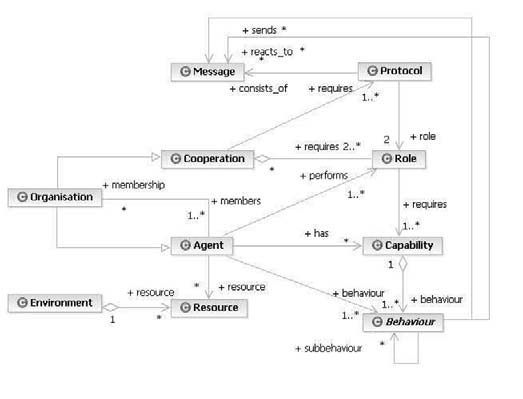
\includegraphics[width=0.6\textwidth]{images/pim4agents/pim4agents-metamodel.png}
	\caption{The PIM4Agents core model \cite{Hahn07b}}
	\label{figure:pim4agents-metamodel}
\end{figure}

%%%%%%%%%%%%%%%%%%%%%%%%%%%%%%%%%%%%%%%%%%%%%%%%%%%%%%%%%%%%%%%%%%%%%%%%%%%%%%%%
\subsection{JadeOrgs}

JadeOrgs
\cite{Madrigal-Mora08} and \cite{Madrigal-Mora09}
is an extension of the Jade framework that implements the JadeMM platform-specific metamodel.

JadeMM is defined using Eclipse Modeling Framework (EMF) to exploit EMF's code generation facility.
Given a platform-independent model of a MAS (conforming to PIM4Agents), the corresponding Jade/JadeOrgs platform-specific model (conforming to JadeMM) can be derived automatically.

%%%%%%%%%%%%%%%%%%%%%%%%%%%%%%%%%%%%%%%%%%%%%%%%%%%%%%%%%%%%%%%%%%%%%%%%%%%%%%%%
%% Title (en): Multiagent Systems and Organizations                           %%
%% Title (cs): Multiagentní systémy a organizace                              %%
%%                                                                            %%
%% Author: Bc. Lukáš Kúdela                                                   %%
%% Supervisor: Prof. RNDr. Petr Štěpánek, DrSc.                               %%
%%                                                                            %%
%% Academic year: 2011/2012                                                   %%
%%%%%%%%%%%%%%%%%%%%%%%%%%%%%%%%%%%%%%%%%%%%%%%%%%%%%%%%%%%%%%%%%%%%%%%%%%%%%%%%

\section{powerJade}

% powerJade - authors
This section introduces the powerJade metamodel
\footnote{The name is intentionally uncapitalized.}
\cite{Baldoni08a}, \cite{Baldoni08b}, \cite{Baldoni09} and \cite{Baldoni10}
put forward in 2008 by Matteo Baldoni, Guido Boella and their colleagues from University of Turin in Turin, Italy.

% Citation
The overview presented here is extracted from the most complete paper on powerJade \cite{Baldoni10}.

%% Summary %%%%%%%%%%%%%%%%%%%%%%%%%%%%%%%%%%%%%%%%%%%%%%%%%%%%%%%%%%%%%%%%%%%%%

% powerJade inspired by powerJava
powerJade is inspired by the authors' previous work on powerJava -- an extension of the Java programming language with an explicit role construct, based on an ontological analysis of roles described in \cite{Baldoni05}, \cite{Baldoni06a}, \cite{Baldoni06b} and \cite{Baldoni07}.

% Definitions (organization, role)
An organization belongs to the social reality and it can only be interacted with via the roles it defines \cite{Boella06}.
Specifically, it is not an object that could be manipulated from outside like objects in OOP.
The concept of organization is useful not only when modelling problem domains including organizations of some kind.
Indeed, we can view every object as an organization offering different ways of interacting with it, each represented by a different role.

%%%%%%%%%%%%%%%%%%%%%%%%%%%%%%%%%%%%%%%%%%%%%%%%%%%%%%%%%%%%%%%%%%%%%%%%%%%%%%%%
\subsection*{Organizational Structure Metamodel}

An ontological analysis of roles in \cite{Boella04} yields the following properties of roles:
\begin{itemize}
	\item \textit{Foundation} -- A role instance is always associated with an instance of the organization class to which is belongs and with a player instance.
	\item \textit{Definitional dependence} -- The definition of a role depends on the organizations it belongs to.
	\item \textit{Institutional powers} -- Role operations (called \textit{powers}) have access to the state of the organization and other roles of the organization.
	\item \textit{Prerequisities} -- To be granted a role, the player must be able to perform operations (called \textit{requirements}) which can be requested while it plays the role.
\end{itemize}


The metmodel in \cite{Boella04} is focused on organizational structure.
% Ontological status of organizations and roles compared to agents
The ontological status of organizations and roles does not differ completely from that of agents or even objects \cite{Boella04}.
% Differences
On one hand, organizations and roles, unlike agents, are not autonomous and act via their members and players.
Additionally, roles, unlike objects, do not exist as independent entities, since they are necessarily linked to organizations.
% Similarities
On the other hand, organizations and roles, like agents, are descriptions of complex behaviour.
In the real world, organizations are considered legal entities; they can even act like agents, albeit via a representative role.
Since they share some properties with agents, they can be modelled using similar primitives.

%%%%%%%%%%%%%%%%%%%%%%%%%%%%%%%%%%%%%%%%%%%%%%%%%%%%%%%%%%%%%%%%%%%%%%%%%%%%%%%%
\subsection*{Role Dynamics Metamodel}

The metamodel in \cite{Dastani04} is focused on role dynamics.
% Four operations: Enact, deact, actiavte, deactivate
Four operations pertaining to the role dynamics are defined: \textit{enact} and \textit{deact} meaning that an agent acquires and relinquishes a role, and \textit{activate} and \textit{deactivate} meaning that the agent actually starts and stops playing a role.
Even though it is possible (and very common) for an agent to be enacting multiple roles simultaneously, only one of these can be active at any moment.
Naturally, it is possible that at some moment none is active.
In particular, when an agent is invoking a power, exactly one of its roles is active.

%%%%%%%%%%%%%%%%%%%%%%%%%%%%%%%%%%%%%%%%%%%%%%%%%%%%%%%%%%%%%%%%%%%%%%%%%%%%%%%%
\subsection*{Unified Metamodel}

The authors of powerJade merged the models in \cite{Boella04} (organization strucure) and \cite{Boella04} (role dynamics) into a unified metamodel.
Organizations and roles are not just design-time abstractions with no run-time projections and players are not just isolated agents; they are all agents interacting with one another.
A logical specification of this unified metamodel can be found in \cite{Boella07}.

%%%%%%%%%%%%%%%%%%%%%%%%%%%%%%%%%%%%%%%%%%%%%%%%%%%%%%%%%%%%%%%%%%%%%%%%%%%%%%%%
\subsection*{Powers and Requirements}

% Role (AOPwO) vs. interace (OOP)
Roles in powerJade can be compared to interfaces from OOP.
Just like an interface is a contract between a calling class and called class, a role is a contract between an organization and an agent.

% OOP: called class implements interfaces vs. powerJade: player enacts roles
% OOP
In OOP, the relationship between a class and the interfaces it implements is a rigid one -- the interfaces a class implements are part of its design-time definition and cannot be implemented or un-implemented at run-time.
% powerJade
In contrast, the relationship between a player and roles it enacts in powerJade is a flexible one -- the roles the a player enacts are not part of its design-time definition and can be enacted and deacted at run-time.

% OOP: interfaces declare methods & events vs. AOPwO: roles define requirements & powers
% OOP
Interfaces in OOP declare methods and events.
When implementing an interface, a class has to implement its methods and it can raise its events.
% powerJade
Similarly, roles in powerJade define \textit{requirements} and \textit{powers}.
When eancting a role, a player has to execute its requirements and it can invoke its powers.
Thus, interface methods correspond to role requirements (both are responsibilities), while interface events are analogous to role powers (both are competences).
%%%%%%%%%%%%%%%%%%%%%%%%%%%%%%%%%%%%%%%%%%%%%%%%%%%%%%%%%%%%%%%%%%%%%%%%%%%%%%%%
%% MASTER'S THESIS                                                            %%
%%                                                                            %% 
%% Title (en): Multi-Agent Systems and Organizations                          %%
%% Title (cs): Multiagentní systémy a organizace                              %%
%%                                                                            %%
%% Author: Bc. Lukáš Kúdela                                                   %%
%% Supervisor: Prof. RNDr. Petr Štěpánek, DrSc.                               %%
%%                                                                            %%
%% Academic year: 2011/2012                                                   %%
%%%%%%%%%%%%%%%%%%%%%%%%%%%%%%%%%%%%%%%%%%%%%%%%%%%%%%%%%%%%%%%%%%%%%%%%%%%%%%%%

\chapter{Platform-Independent Metamodel---Thespian}

% Chapter intro
In this chapter, we will present our platform-independent metamodel for modelling organizations in MASs---\textit{Thespian}.

% Thespian - defnition
\textit{Thespian} is a metamodel to which platform-independent models of organizations in MASs must conform; in more detail, it is a model\footnote{Recall that a metamodel is a kind of model.} representing a modelling language \footnote{When can call this language the \textit{Thespian modelling language}.} to which platform-independent models of organizations in MASs must conform.

% Thespian name inspiration - Thespis of Icaria
\textit{Thespian} is named after \textit{Thespis of Icaria} (present-day Dionysos, Greece), who lived in the 6th century BC and, according to certain Ancient Greece sources and especially Aristotle, was the first person ever to appear on stage as an actor playing a character in a play (instead of just speaking as himself) \cite{Wikipedia-Thespis}.

% Thespian inspiration - Aalaadin, O&P, PIM4Agents and powerJade
\textit{Thespian} is inspired by all four metamodels introduced in the previous chapter: \textit{Aalaadin}, \textit{O\&P}, \textit{PIM4Agents} and \textit{powerJade}.
% Aaalaadin
Similarly to \textit{Aalaadin}, it contains both dynamic and static concepts (called \textit{core} and \textit{methodological} concepts in Aalaadin).
Instances of dynamic/static concepts will end up as run-time/design-time entities in the platform-specific model.
% O&P
Like \textit{O\&P}, it can be used to model holonic MASs.
% PIM4Agents
Similarly to \textit{PIM4Agents}, it enables explicit modelling of protocols and messages exchanged in these protocols.
% powerJade 
And finally like \textit{powerJade}, it is able to represent competences and responsibilities (called \textit{powers} and \textit{requirements} respectively in \textit{powerJade}) of roles.

% Two partitions: {organization, player and protocol}, {desgn-time and run-time}
The \textit{Thespian} metamodel can be partitioned in two orthogonal ways: in a high-level and low-level way.
Both partitions will be described in the following sections; the integrated metamodel will be presented in the last section.

% High-level partition
The high-level partition divides the concepts according to the area they represent: organization, player or protocol.
This is a more natural partition of the two since fewer dependencies among concepts from different parts exists than in the other partition.
The organization/protocol part of the MAS can be designed (and implemented) independently of the player part; indeed agent developed by one team can become members of organizations and play roles developed by another team. 

% Low-level partition
The low-level partition separates the concepts based on whether they represent design-time or run-time entities.
The design-time entities are created already at design-time and are usually implemented as \textit{agent classes} in the target agent platform; they are analogous to the concept of \textit{Class} in OOP.
The run-time entities are created only at run-time and are usually implemented as \textit{agent instances} in the target agent platform; they are analogous to the concept of \textit{Instance} in OOP.

% Type-token distinction - definition
Before continuing with the presentation of \textit{Thespian}, it is important to explain the \textit{type-token distinction}.
In disciplines such as philosophy and knowledge representation, the type-token distinction is a distinction that separates a \textit{concept} from objects that are particular \textit{instances} of that concept.
\textit{Thespian} has been designed to support the type-token distinction and the correct differentiation is a recurring theme in this chapter.

% Type-token distinction - MAS
As an example of the type-token distinction, consider a MAS.
The \textit{specification} of the MAS (its source code) is the \textit{MAS type} and its \textit{manifestation} (a running MAS) is the \textit{MAS token}.
Just like a type can (and usually does) have many tokens, a MAS specification can have multiple manifestations---the same source code can be run many times.

% Static & dynamic metamodels
The \textit{Thespian} metamodel includes both a static and dynamic metamodels for describing structural and behavioural aspects of organizations respectively.
In the following two sections, we will introduce both metamodels in detail.

%%%%%%%%%%%%%%%%%%%%%%%%%%%%%%%%%%%%%%%%%%%%%%%%%%%%%%%%%%%%%%%%%%%%%%%%%%%%%%%%
%% MASTER'S THESIS                                                            %%
%%                                                                            %% 
%% Title (en): Multi-Agent Systems and Organizations                          %%
%% Title (cs): Multiagentní systémy a organizace                              %%
%%                                                                            %%
%% Author: Bc. Lukáš Kúdela                                                   %%
%% Supervisor: Prof. RNDr. Petr Štěpánek, DrSc.                               %%
%%                                                                            %%
%% Academic year: 2011/2012                                                   %%
%%%%%%%%%%%%%%%%%%%%%%%%%%%%%%%%%%%%%%%%%%%%%%%%%%%%%%%%%%%%%%%%%%%%%%%%%%%%%%%%

\section{Static Metamodel}

The static \textit{Thespian} metamodel is used to model static (structural) aspects of OCMAS like:
\begin{itemize}
	\item an organization's role structure and protocols,
	\item a role's competences and responsibilities or
	\item a player's capabilities.
\end{itemize}

%%%%%%%%%%%%%%%%%%%%%%%%%%%%%%%%%%%%%%%%%%%%%%%%%%%%%%%%%%%%%%%%%%%%%%%%%%%%%%%%
\subsection{Organization Metamodel}

% Organization metamodel - usage
The Organization metamodel (figure~\ref{figure:thespian-organization-metamodel}) contains concepts whose instances model organizations and roles with their competences and responsibilities.

\subsubsection*{Organization and Organization Type}

% Type-token distinction - organization
To enable the type-token distinction, \textit{Thespian} contains concepts for modelling both an \textit{organization type} and an \textit{organization token}: \textit{Organization type} and \textit{Organization}.

% Organization
\textit{Organization} (also called \textit{Organization instance}) is an actual organization in a running MAS; it is a run-time entity.
% Organization - state
It is classified by an \textit{Organization type} which specifies its role structure.
% Organization - note
Note that despite an organization being a run-time entity, it can be declared at design-time, created at MAS start-up and destroyed at MAS shut-down.

% Organization type
\textit{Organization type} (also called \textit{Organization class}) is a class of organizations sharing the same role structure; it is a design-time entity.
% Organization type - state
It contains a set of \textit{Roles} defining its role structure.
% Organization type - behaviour
It can be instantiated to yield an \textit{Organization}. 

\subsubsection*{Role and Position}

% Type-token distinction - role
\textit{Thespian} contains concepts for modelling both an \textit{role type} and \textit{role token} to enable the type-token distinction: \textit{Role} and \textit{Position}.

% Role
\textit{Role} is a role specification within an organization; it is a design-time entity.
% Role - state
It has a set of \textit{Competences} and a set of \textit{Responsibilities} defining its function in its containing \textit{Organization type} and multiplicity differentiating between a \textit{single role})---one that can not be played by more than one \textit{Player} in an \textit{Organization}---and a \textit{multiple role}---one that can.
Currently, neither \textit{Thespian} not \textit{Thespian4Jade} support differentiating between a \textit{mandatory role}---one that has to be played at all times---and an \textit{optional role}---one that does not have to be.

% Position
A \textit{Position} (sometimes called \textit{Role instance}) is a role realization within an actual organization; it is a run-time entity.
% Position - state
It is a realization of \textit{Role} which specifies its competences
It belongs to an \textit{Organization} and is played by a \textit{Player}.
% Position - note
Note that a \textit{Position} is usually not declared at design-time; it is created when an \textit{Player} starts playing a role in an \textit{Organization} and destroyed when that \textit{Player} stops doing so.

\subsubsection*{Competence and Responsibility}

Let us consider a player playing a role.
As a result of playing the role, the player gains competences a responsibilities associated with that role.

% Competence
\textit{Competence} is an operation a player playing a role \textit{can} can execute as a result of playing that role; it is a design-time entity.
% Competence - state
A \textit{Competence} can require an argument from a player after its invocation (but before its execution), in which case the argument type (a Java type) has to be specified.
Also it can provide a return value to the player after its execution, in which case the return value type (a Java type) has to be specified.

% Figure: Thespian - Organization metamodel
\begin{figure}[ht]
	\centering
	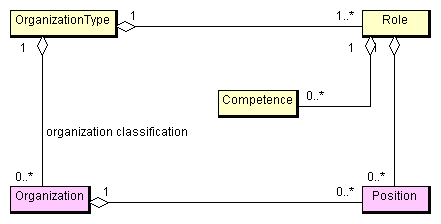
\includegraphics[width=0.8\textwidth]{images/thespian/organization-metamodel.png}
	\caption{The Organization metamodel}
	\label{figure:thespian-organization-metamodel}
\end{figure}

%%%%%%%%%%%%%%%%%%%%%%%%%%%%%%%%%%%%%%%%%%%%%%%%%%%%%%%%%%%%%%%%%%%%%%%%%%%%%%%%
\subsection{Player Metamodel}

% Player metamodel - usage
The Player metamodel (figure~\ref{figure:thespian-player-metamodel}) contains constructs for modelling players and their responsibilities.

\subsubsection*{Player and Player Type}

% Type-token distinction - player
To facilitate the type-token distinction, \textit{Thespian} contains concepts for modelling both a \textit{player type} and a \textit{player token}: \textit{Player type} and \textit{Player}.

% Player
\textit{Player} is an actual player in a running MAS; it is a run-time entity.
% Player - state
It is classified by a player type which specifies its responsibilities.
% Player - note
Note that despite a player being a run-time entity, it has to be declared at design-time, created at MAS start-up and destroyed at MAS shut-down.

% Player type
\textit{Player type} (also called \textit{Player class})is a class of players sharing the same characteristics, namely responsibilities; it is a design-time entity.
% Player type - state
It has a set of responsibilities defining its capabilities when playing a role.
% Player type - behaviour
It can be instantiated to yield a player. 

\subsubsection*{Responsibility}

% Responsibility
\textit{Responsibility}is an operation a player playing a role \textit{must} execute as a result of playing that role; it is a design-time entity. 
% Responsibility - state
A \textit{Responsibility} can provide an argument to a player after its invocation (but before its execution), in which case the argument type (a Java type) has to be specified.
Also it can request a return value from the player after its execution, in which case the return value type (a Java type) has to be specified.

% Figure: Thespian - Player metamodel
\begin{figure}[ht]
	\centering
	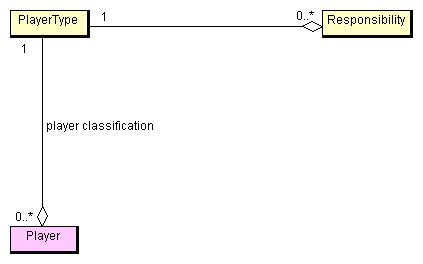
\includegraphics[width=0.4\textwidth]{images/thespian/player-metamodel.png}
	\caption{The Player metamodel}
	\label{figure:thespian-player-metamodel}
\end{figure}

%%%%%%%%%%%%%%%%%%%%%%%%%%%%%%%%%%%%%%%%%%%%%%%%%%%%%%%%%%%%%%%%%%%%%%%%%%%%%%%%
\subsection{Protocol Metamodel}

% Protocol metamodel - usage
The Protocol metamodel (figure~\ref{figure:thespian-protocol-metamodel}) contains abstractions whose instances represent interaction protocols between a player and an organization or role, and among roles themselves.

\subsubsection*{Protocol}

% Protocol
An \textit{Interaction protocol} is an institutionalized pattern of interaction (communication) between two or more roles within an organization; it is a design-time entity modelled by the \textsc{Protocol} class.
It defines parties involved in the interaction and messages exchanged in the communication.

% Scenario
A realization of an interaction protocol is an \textit{Interaction scenario}---a sequence of actions performed (messages exchanged) by two or more roles within an organization; a scenario is a purely run-time entity.
In other words, a protocol is a framework and a scenario (is) one of its possible instantiations.
Since scenarios are usually not explicitly modelled\footnote{Scenarios can be explicitly modelled in snapshots.}, \textit{Thespian} does not contain the concept of an \textit{Interaction scenario}.

% Type-token distinction - protocol
The theme of type-token distinction is at play here: instances of \textit{Protocol} model \textit{protocol types} and instances of \textit{Scenario} represent \textit{protocol tokens}.

\subsubsection*{Party}

% Party - definition
A \textit{Party} is a role involved in a protocol; it is a design-time entity modelled by the \textsc{Party} abstract class.
A relationship between roles and protocols is a many-to-many one; a role can participate in multiple protocols and at least two different roles have to take part in a protocol; a party is a reification (embodiment) of this relationship.
% Initiator party & Responder party
A \textit{Party} is either an \textit{Initiator party}---one that initiates the protocol---or a \textit{Responder party}---one that responds to the initiated protocol. These two concepts are modelled by two concrete classes: \textsc{InitiatorParty} and \textsl{ResponderParty} respectively.

\subsubsection*{Message}

A \textit{Message} is a piece of information exchanged between two parties in a protocol; it is a design-time entity modelled by the \textsc{Message} class.

% Figure: Thespian - Protocol metamodel
\begin{figure}[ht]
	\centering
	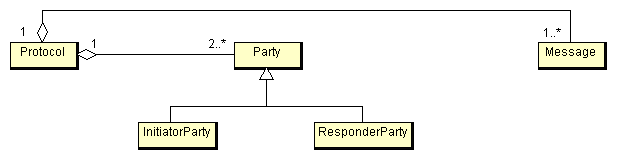
\includegraphics[width=0.8\textwidth]{images/thespian/protocol-metamodel.png}
	\caption{The Protocol metamodel}
	\label{figure:thespian-protocol-metamodel}
\end{figure}

%%%%%%%%%%%%%%%%%%%%%%%%%%%%%%%%%%%%%%%%%%%%%%%%%%%%%%%%%%%%%%%%%%%%%%%%%%%%%%%%
\subsection{Compile-Time Metamodel}	

% Design-time metamodel - usage
The Design-time metamodel contains concepts whose instances model the design-time MAS entities.
These entities, as their name suggests, are created and/or modified at design-time by the MAS designer, and they constitute the MAS specification (see this chapter's introduction).
The models of MAS specifications are also called \textit{static MAS models}.

% Figure: Thespian - Compie-time metamodel
\begin{figure}[ht]
	\centering
	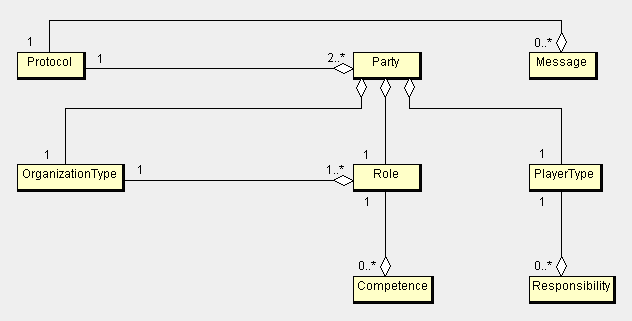
\includegraphics[width=0.8\textwidth]{images/thespian/compile-time-metamodel.png}
	\caption{The Compile-time metamodel}
	\label{figure:thespian-static-metamodel}
\end{figure}

%%%%%%%%%%%%%%%%%%%%%%%%%%%%%%%%%%%%%%%%%%%%%%%%%%%%%%%%%%%%%%%%%%%%%%%%%%%%%%%%
\subsection{Run-Time Metamodel}

% Run-time metamodel - usage
The Run-time metamodel contains constructs that model the run-time MAS entities.
These entities, as their name implies, are created and/or modified at run-time by the MAS itself, and they make up the MAS manifestation (see this chapter's introduction).
They models of MAS manifestations are also referred to as \textit{dynamic MAS models} or \textit{MAS snapshots}.

% Figure: Thespian - Run-time metamodel
\begin{figure}[ht]
	\centering
	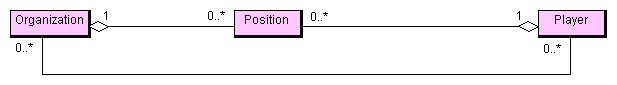
\includegraphics[width=0.8\textwidth]{images/thespian/run-time-metamodel.png}
	\caption{The Run-time metamodel}
	\label{figure:thespian-dynamic-metamodel}
\end{figure}

%%%%%%%%%%%%%%%%%%%%%%%%%%%%%%%%%%%%%%%%%%%%%%%%%%%%%%%%%%%%%%%%%%%%%%%%%%%%%%%%
\subsection{Integrated Metamodel}

Figure~\ref{figure:thespian-integrated-metamodel} shows the integrated \textit{Thespian} metamodel.

% Key property of Thespian - no association between Role and Player type
We would like to emphasize what we perceive as key property of \textit{Thespian}: there is no association between \textit{Role} and \textit{Player type}, no link between a specific role and a particular player type.
This means that there is no design-time dependency between roles and player types; all connections arise at run-time and happen between positions and players.

% Figure: Thespian integrated metamodel
\begin{figure}[ht]
	\centering
	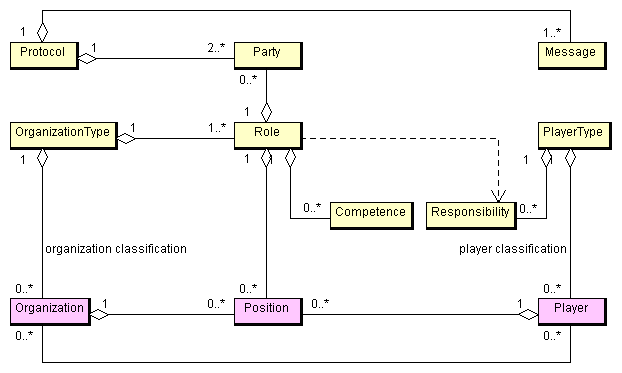
\includegraphics[width=0.8\textwidth]{images/thespian/thespian-metamodel.png}
	\caption{The Integrated metamodel}
	\label{figure:thespian-integrated-metamodel}
\end{figure}

%%%%%%%%%%%%%%%%%%%%%%%%%%%%%%%%%%%%%%%%%%%%%%%%%%%%%%%%%%%%%%%%%%%%%%%%%%%%%%%%
%% MASTER'S THESIS                                                            %%
%%                                                                            %% 
%% Title (en): Multi-Agent Systems and Organizations                          %%
%% Title (cs): Multiagentní systémy a organizace                              %%
%%                                                                            %%
%% Author: Bc. Lukáš Kúdela                                                   %%
%% Supervisor: Prof. RNDr. Petr Štěpánek, DrSc.                               %%
%%                                                                            %%
%% Academic year: 2011/2012                                                   %%
%%%%%%%%%%%%%%%%%%%%%%%%%%%%%%%%%%%%%%%%%%%%%%%%%%%%%%%%%%%%%%%%%%%%%%%%%%%%%%%%

\section{Dynamic Metamodel}

The dynamic Thespian metamodel is used to model dynamic (behavioural) aspects of OCMAS like:
\begin{itemize}
	\item players playing roles within organizations,
	\item players exercising their roles' competences and fulfilling their roles' responsibilities, or
	\item players subscribing to organization events, or
	\item organizations publishing events.
\end{itemize}

%%%%%%%%%%%%%%%%%%%%%%%%%%%%%%%%%%%%%%%%%%%%%%%%%%%%%%%%%%%%%%%%%%%%%%%%%%%%%%%%
\subsection{Player and Organization Interaction}

% Organization protocols
A player and an organization interact through four protocols: \textit{Enact role}, \textit{Deact role}, \textit{Subscribe to event} and \textit{Publish event}.

%%%%%%%%%%%%%%%%%%%%%%%%%%%%%%%%%%%%%%%%%%%%%%%%%%%%%%%%%%%%%%%%%%%%%%%%%%%%%%%%
\subsubsection{Enacting a Role}

% Figure: 'Enact role' protocol
\begin{figure}[ht]
	\centering
	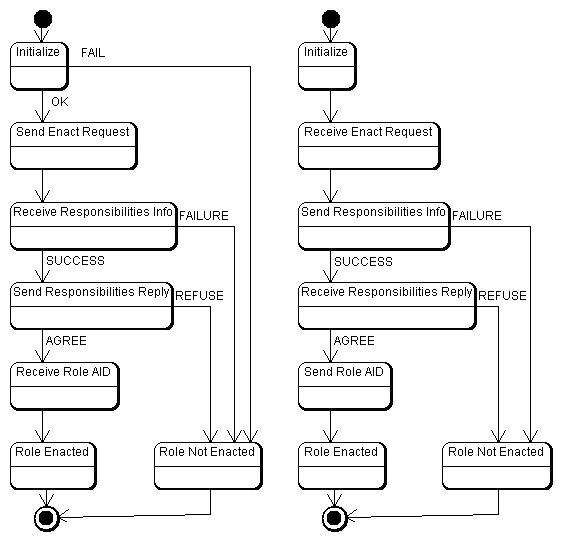
\includegraphics[width=0.8\textwidth]{images/thespian/enact-role-protocol.png}
	\caption{The \textit{Enact role} protocol}
	\label{figure:thespian-enact-role-protocol}
\end{figure}

% 'Enact a role in an organization' - definition
To \textit{enact} a role in an organization means to assume a in an organization.
% Restrictions
Naturally, only a non-enacted or multiple role can be enacted; more precisely, a role can only be enacted in a concrete organization in which it is not already enacted by any player or is defined as a multiple role.
% Protocol
A player who wants to enact a role in an organization, initiates the \textit{Enact role} protocol with that organization.

% 'Enact role' protocol - definition
The \textit{Enact role} protocol consists of the following steps:
\begin{enumerate}
	% 1
	\item The player sends an \textit{Enact role request} message to the organization containing the name of the role it wants to enact.
	% 2	
	\item The organization receives the request message and sends back either
	\begin{itemize}
		% SUCCESS
		\item a \textit{Required Responsibilities} message listing the role's responsibilities if such role exists and can be enacted, i.e. if it is not enacted by any player or is defined as a multiple role, or
		% Failure
		\item a \textit{Failure} message otherwise. 
	\end{itemize}
	% 3	
	\item Upon receiving a \textit{Required Responsibilities} message, the player then determines if it has the required capabilities to fulfil the role's responsibilities and replies either with
	\begin{itemize}
		% AGREE		
		\item an \textit{Agree} message if it has the capabilities, or
		% REFUSE
		\item a \textit{Refuse} message otherwise.
	\end{itemize}
	% 4
	\item Upon receiving an \textit{Agree} message, the organization creates a position and sends a \textit{Role AID} message containing its AID to the player.
	The organization then ends its part in the protocol.
	% 5
	\item The player receives the \textit{Role AID} message and ends its part in the protocol.
\end{enumerate}


%%%%%%%%%%%%%%%%%%%%%%%%%%%%%%%%%%%%%%%%%%%%%%%%%%%%%%%%%%%%%%%%%%%%%%%%%%%%%%%%
\subsubsection{Deacting a Role}

% Figure: 'Deact role' protocol
\begin{figure}[ht]
	\centering
	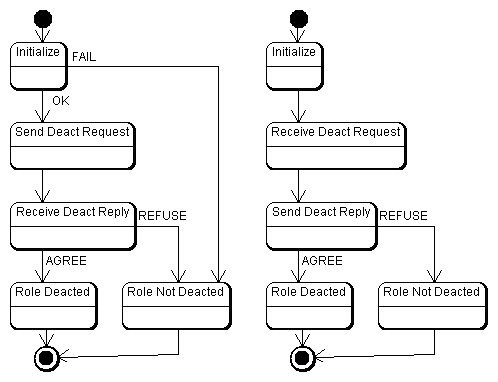
\includegraphics[width=0.8\textwidth]{images/thespian/deact-role-protocol.png}
	\caption{The \textit{Deact role} protocol}
	\label{figure:thespian-deact-role-protocol}
\end{figure}

% 'Deact a role in an organization' - definition
To \textit{deact}
\footnote{The word `deact' does not exist in the English language, it is a made-up word.}
a role in an organization means to relinquish a role in an organization.
% Restrictions
Naturally, only an enacted and inactive (see section~\ref{section:activating-a-role} for details) role can be deacted; more precisely, a role can only be deacted in a concrete organization in which it is enacted by the player and inactive.
% Protocol
A player who wants to deact a role in an organization, initiates the \textit{Deact role} protocol with that organization.

% 'Deact role' protocol - definition
The following steps comprise the \textit{Deact role} protocol:
\begin{enumerate}
	% 1
	\item The player sends a \textit{Deact role request} message to the organization containing the name of the role it wants to enact.
	% 2	
	\item The organization receives the request message and sends back either
	\begin{itemize}
		% AGREE
		\item an \textit{Agree} message if the role exists and can be deacted, i.e. if it is enacted by the player and inactive, or
		% REFUSE
		\item a \textit{Refuse} message otherwise. 
	\end{itemize}
	The organization then ends its part in the protocol.
	% 3
	\item The player receives the reply message and ends its part in the protocol.
\end{enumerate}

%%%%%%%%%%%%%%%%%%%%%%%%%%%%%%%%%%%%%%%%%%%%%%%%%%%%%%%%%%%%%%%%%%%%%%%%%%%%%%%%
\subsubsection{Subscribing to an Event}

% Figure: 'Subscribe to event' protocol
\begin{figure}[ht]
	\centering
	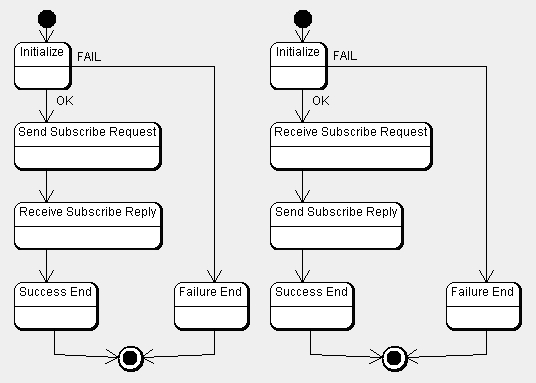
\includegraphics[width=0.8\textwidth]{images/thespian/subscribe-to-event-protocol.png}
	\caption{The \textit{Subscribe to event} protocol}
	\label{figure:thespian-subscribe-to-event-protocol}
\end{figure}

% 'Subscribe to an event in an organization' - definition
Subscribing to an event in an organization means to be notified of an event in an organization.
A player can subscribe to the \textit{role enacted}, \textit{role deacted}, \textit{role activated} and \textit{role deactivated} events raised when a role is enacted, deacted, activated and deactivated respectively.
% Restrictions
Naturally, only an employed player can subscribe to an event; more precisely, an event can only be subscribed to in a concrete organization in which the player enacts a role.
% Protocol
A player who wants subscribe to an event in an organization, initiates the \textit{Subscribe to event} protocol with that organization.

% 'Subscribe to event' protocol - definition
The \textit{Subscribe to event} protocol consists of the following steps:
\begin{enumerate}
	% 1
	\item The player sends a \textit{Subscribe to event request} message containing the name of the role it wants to enact to the organization.
	% 2	
	\item The organization receives the request message and immediately terminates if the message comes from a player that is not employed by that organization.
	If the message comes from a player employed in that organization, it sends back either
	\begin{itemize}
		% AGREE
		\item an \textit{Agree} message if the event exists, or
		% REFUSE
		\item a \textit{Refuse} message otherwise. 
	\end{itemize}
	The organization then ends its part in the protocol.
	% 3
	\item The player receives the reply message and ends its part in the protocol.
\end{enumerate}

%%%%%%%%%%%%%%%%%%%%%%%%%%%%%%%%%%%%%%%%%%%%%%%%%%%%%%%%%%%%%%%%%%%%%%%%%%%%%%%%
\subsubsection{Publishing an Event}

% Figure: 'Publish event' protocol
\begin{figure}[ht]
	\centering
	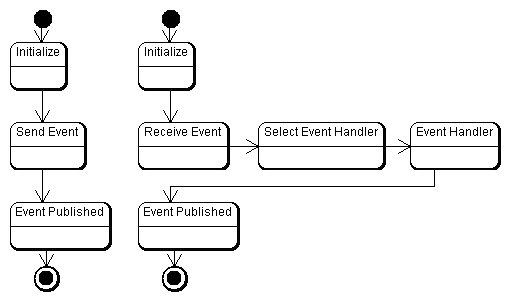
\includegraphics[width=0.8\textwidth]{images/thespian/publish-event-protocol.png}
	\caption{The \textit{Publish event} protocol}
	\label{figure:thespian-publish-event-protocol}
\end{figure}

% 'Publishing an event to subscribed players' - definition
To publish an event to its subscribers means to notify the players subscribed to an event of that event occurring.
% Restrictions
% - none
% Protocol
An organization that wants publish an event to its subscribers, initiates the \textit{Publish event} protocol with the event subscribers.

% 'Publish event' protocol - definition
The following steps comprise the \textit{Publish event} protocol:
\begin{enumerate}
	% 1	
	\item The organization sends an \textit{Event} message containing the name of the event and its argument to the event subscribers.
	The organization then ends its part in the protocol.
	% 2
	\item A subscriber receives the message and handles the event.
	The subscriber then ends its part in the protocol.
\end{enumerate}

%%%%%%%%%%%%%%%%%%%%%%%%%%%%%%%%%%%%%%%%%%%%%%%%%%%%%%%%%%%%%%%%%%%%%%%%%%%%%%%%
\subsection{Player and Role Interaction}

% Role protocols
A player and a role interact via four protocols: \textit{Activate role}, \textit{Deactivate role}, \textit{Invoke competence} and \textit{Invoke responsibility}.

%%%%%%%%%%%%%%%%%%%%%%%%%%%%%%%%%%%%%%%%%%%%%%%%%%%%%%%%%%%%%%%%%%%%%%%%%%%%%%%%
\subsubsection{Activating a Role}
\label{section:activating-a-role}

% Figure: 'Activate role' protocol
\begin{figure}[ht]
	\centering
	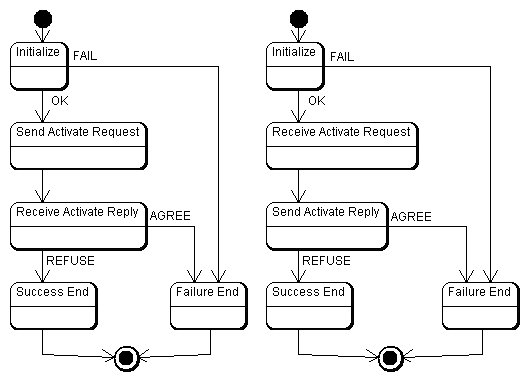
\includegraphics[width=0.8\textwidth]{images/thespian/activate-role-protocol.png}
	\caption{The \textit{Activate role} protocol}
	\label{figure:thespian-activate-role-protocol}
\end{figure}

% 'Activate a role' - definition
To \textit{activate} a role
\footnote{More precisely, what is activated is a position -- a concrete instantiation of a role in a specific organization enacted by the activating player.}
means to begin playing a role, i.e. start exercising its competences and fulfilling its responsibilities.
% Restrictions
Naturally, only an enacted and inactive role can be activated; more precisely, a role can only be activated in a concrete organization in which it is already enacted by the player and inactive.
Furthermore, a player may activate only one role (in all concrete organizations) at a time.
% Protocol
A player who wants to activate a role, initiates the \textit{Activate role} protocol with that role.

% 'Activate role' protocol - definition
The \textit{Activate role} protocol consists of the following steps:
\begin{enumerate}
	% 1
	\item The player sends a \textit{Activate role} request message to the role.
	% 2	
	\item The role receives the request message and immediately terminates if the message comes from anyone else than its player.
	If the message comes from its enacting player, it sends back either
	\begin{itemize}
		% AGREE
		\item an \textit{Agree} message if the role can be activated, i.e. it is inactive, and the player does not have any other active role in the role's organization.
		% REFUSE
		\item a \textit{Refuse} message otherwise. 
	\end{itemize}
	The role then ends its part in the protocol.
	% 3
	\item The player receives the reply message and ends its part in the protocol.
\end{enumerate}

%%%%%%%%%%%%%%%%%%%%%%%%%%%%%%%%%%%%%%%%%%%%%%%%%%%%%%%%%%%%%%%%%%%%%%%%%%%%%%%%
\subsubsection{Deactivating a Role}

% Figure: 'Deactivate role' protocol
\begin{figure}[ht]
	\centering
	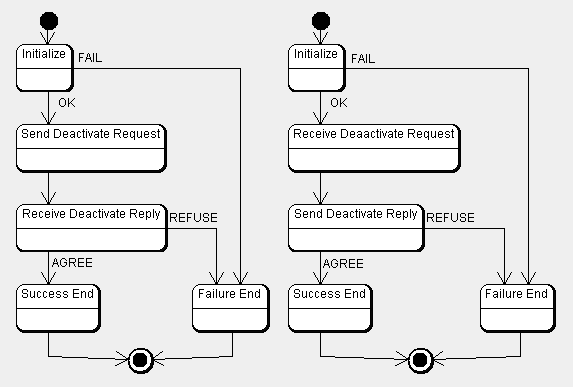
\includegraphics[width=0.8\textwidth]{images/thespian/deactivate-role-protocol.png}
	\caption{The \textit{Deactivate role} protocol}
	\label{figure:thespian-deactivate-role-protocol}
\end{figure}

% 'Deactivating a role' - definition
To \textit{deactivate} a role (more precisely, a position) means to stop playing a role, i.e. stop exercising its competences and fulfilling its responsibilities.
% Restrictions
Naturally, only an enacted and active role can be deactivated; more precisely, a role can only be deacted in a concrete organization in which it is enacted by the player and active.
% Protocol
A player who wants to deactivate a role, initiates the \textit{Deactivate role} protocol with that role.

% 'Deactiavte role' protocol - definition
The following steps comprise the \textit{Deactivate role} protocol:
\begin{enumerate}
	% 1
	\item The player sends a \textit{Deactivate role} request message to the role.
	% 2	
	\item The role receives the request message and immediately terminates if the message comes from anyone else than its player.
	If the message comes its enacting player, it sends back either
	\begin{itemize}
		% AGREE
		\item an \textit{Agree} message if the role can be deactivated, i.e. it is active, or
		% REFUSE
		\item a \textit{Refuse} message otherwise. 
	\end{itemize}
	The role then ends its part in the protocol.
	% 3
	\item The player receives the reply message and ends its part in the protocol.
\end{enumerate}

%%%%%%%%%%%%%%%%%%%%%%%%%%%%%%%%%%%%%%%%%%%%%%%%%%%%%%%%%%%%%%%%%%%%%%%%%%%%%%%%
\subsubsection{Invoking a Competence}

% Figure: 'Invoke competence' protocol
\begin{figure}[ht]
	\centering
	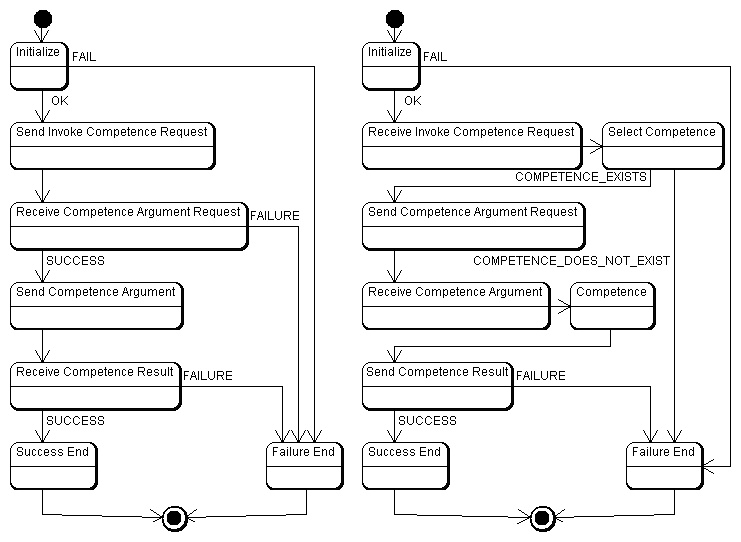
\includegraphics[width=0.8\textwidth]{images/thespian/invoke-competence-protocol.png}
	\caption{The \textit{Invoke competence} protocol}
	\label{figure:thespian-invoke-competence-protocol}
\end{figure}

% 'Invoke a competence on a role' - definition
Invoking a competence on a role (more precisely, a position) happens when a player calls upon its active role to exercise a competence.
% Restrictions
Note that a competence can only be invoked on an active role.
% Protocol
A player who wants to invoke a competence on a role, initiates the \textit{Invoke competence} protocol with that role.

% 'Invoke competence' protocol - definition
The \textit{Invoke competence} protocol consists of the following steps:
\begin{enumerate}
	% 1	
	\item The player sends an \textit{Invoke competence request} request to the role containing the name of the competence to invoke.
	% 2
	\item The role receives the request message and immediately terminates if the message comes from anyone else than its player or it is not active.
	If, on the other hand, the message comes from its player and it is active, it sends back 
	\begin{itemize}
		% SUCCES		
		\item a \textit{Competence argument request} message asking the player to provide the competence argument if the competence exists, or
		% FAILURE
		\item a \textit{Failure} message otherwise. 
	\end{itemize}
	% 3	
	\item Upon receiving the \textit{Competence argument request} message, the player sends the \textit{Competence argument} message carrying the competence argument.
	% 4
	\item The role receives the competence argument and executes the competence and sends back either
	\begin{itemize}
		% SUCCESS
		\item either a \textit{Competence result} message carrying the competence result in case the competence executed successfully, or
		\item a \textit{Failure} message otherwise.
	\end{itemize}
	The role then ends its part in the protocol.
	% 5
	\item The player receives the reply message and ends its part in the protocol.
\end{enumerate}

%%%%%%%%%%%%%%%%%%%%%%%%%%%%%%%%%%%%%%%%%%%%%%%%%%%%%%%%%%%%%%%%%%%%%%%%%%%%%%%%
\subsubsection{Invoking a Responsibility}

% Figure: 'Invoke responsibility' protocol
\begin{figure}[ht]
	\centering
	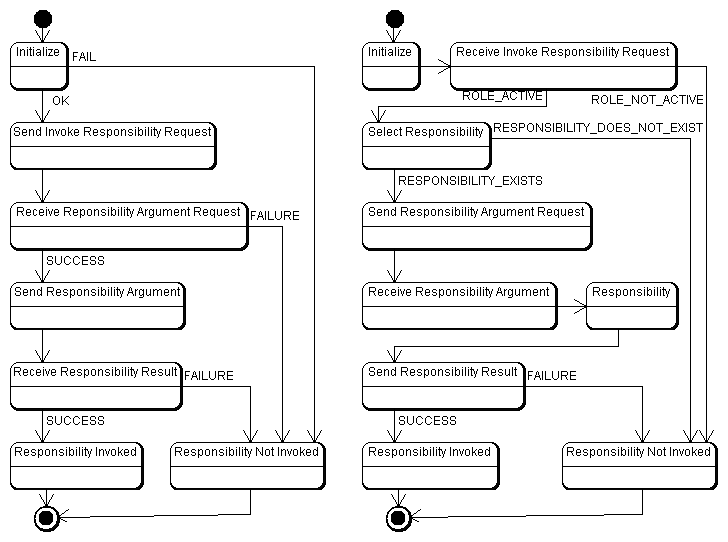
\includegraphics[width=0.8\textwidth]{images/thespian/invoke-responsibility-protocol.png}
	\caption{The \textit{Invoke responsibility} protocol}
	\label{figure:thespian-invoke-responsibility-protocol}
\end{figure}

% 'Invoke a responsibility on a player' - definition
Invoke a responsibility on a player happens when a role (more precisely, a position) calls upon its player to fulfil a responsibility.
% Restrictions
Note that a responsibility can only be invoked by an active role.
% Protocol
A role who wants to invoke a responsibility on its player, initiates the \textit{Invoke responsibility} protocol with its player.

% 'Invoke responsibility' protocol - definition
The following steps comprise the \textit{Invoke responsibility} protocol:
\begin{enumerate}
	% 1	
	\item The role sends an \textit{Invoke responsibility request} request to the role containing the name of the responsibility to invoke.
	% 2
	\item The player receives the request message and immediately terminates if the message comes from anyone else than its active role.
	If, on the other hand, the message comes from its active role, it sends back 
	\begin{itemize}
		% SUCCES		
		\item a \textit{Responsibility argument request} message asking the role to provide the responsibility argument if the responsibility exists, or
		% FAILURE
		\item a \textit{Failure} message otherwise. 
	\end{itemize}
	% 3	
	\item Upon receiving the \textit{Responsibility argument request} message, the role sends the \textit{Responsibility argument} message carrying the responsibility argument.
	% 4
	\item The player receives the responsibility argument and executes the responsibility and sends back either
	\begin{itemize}
		% SUCCESS
		\item a \textit{Responsibility result} message carrying the responsibility result in case the responsibility executed successfully, or
		\item a \textit{Failure} message otherwise.
	\end{itemize}
	The player then ends its part in the protocol.
	% 5
	\item The role receives the reply message and ends its part in the protocol.
\end{enumerate}
%%%%%%%%%%%%%%%%%%%%%%%%%%%%%%%%%%%%%%%%%%%%%%%%%%%%%%%%%%%%%%%%%%%%%%%%%%%%%%%%
%% Title (en): Multiagent Systems and Organizations                           %%
%% Title (cs): Multiagentní systémy a organizace                              %%
%%                                                                            %%
%% Author: Bc. Lukáš Kúdela                                                   %%
%% Supervisor: Prof. RNDr. Petr Štěpánek, DrSc.                               %%
%%                                                                            %%
%% Academic year: 2011/2012                                                   %%
%%%%%%%%%%%%%%%%%%%%%%%%%%%%%%%%%%%%%%%%%%%%%%%%%%%%%%%%%%%%%%%%%%%%%%%%%%%%%%%%

\chapter{Metamodel Implementation -- Thespian4Jade}

% Chapter abstract - Thespian4Jade
In this chapter, we will present Thespian4Jade -- an implementation of Thespian for the Jade agent platform.
Thespian4Jade defines classes that can be subclassed to build platform-specific models of OCMASs.

%%%%%%%%%%%%%%%%%%%%%%%%%%%%%%%%%%%%%%%%%%%%%%%%%%%%%%%%%%%%%%%%%%%%%%%%%%%%%%%%
\section{Agent Platform}

% About agent platforms
There are numerous agent platforms available including proprietary, free/open source, and public domain software.

% General vs. specific agent plaforms
The primary distinguishing factor among them is the degree of generality.
The most general among the agent platforms do not impose any particular agent architecture and usually pick a general-purpose programming language (typically the Java programming language) as their agent programming language.
On the other hand, the least general (or more generously -- most specific) agent platforms do prescribe a concrete agent architecture and generally make use of some (declarative) domain-specific language.

% Why Jade?
As our aim was to introduce organizational concepts as first-class citizens in the MAS landscape, we had to steer towards the agent platform offering the most extension points.
Therefore, we considered only the most general free and open source agent platforms.
Finally we picked the Jade platform (described in the following section) which, at the time of writing this thesis, appears to be the community choice number one.  

%%%%%%%%%%%%%%%%%%%%%%%%%%%%%%%%%%%%%%%%%%%%%%%%%%%%%%%%%%%%%%%%%%%%%%%%%%%%%%%%
\section{Jade}

% Jade an agent platform and framework in one
Jade (Java Agent Development Framework) is an agent platform and framework in one.

% Jade as agent platform
It is a \textit{platform} because it provides a run-time environment in which the agents operate, much like a sandbox in which children play.
Jade also manages the lifetimes of the agents running on the platform, delivers messages (asynchronous message passing) and provides other services (e.g. the yellow pages service).

% Jade as a framework
Jade is also a \textit{framework} because it comes with an extensive base class libraries and the actual user-defined classes are expected to inherit from these base classes, much like a building is expected to be built within the boundaries of an already erected scaffolding.
A concrete multiagent system is basically an instantiation of the Jade as a framework.

% About Jade
Jade simplifies the implementation of multiagent systems by acting as a middleware that complies with the FIPA
[FIPA: http://www.fipa.org]
specifications
[FIPA-Specificaiton: http://www.fipa.org/specifications/index.htmls] and by providing a set of graphical tools that support the debugging and deployment phases.
The agent platform can be distributed across multiple machines (possibly running different operating systems) and it can be configured via a remote graphical tool.
The configuration can be even changed at run-time by moving agents from one machine to another, as and when required. 
Jade is written in the Java programming language. 

% Extensibility
Jade has been specifically designed with extensibility in mind and since our goal is to extend the multiagent systems with organizational concepts, this is the platform of our choice.
The fact that it places great emphasis on extensibility also manifests in its choice of the actual agent programming language -- the Java programming language.

% Minimalistic architecture
A feature of Jade we find particularly noteworthy is its minimalistic architecture.
Only the most fundamental services (e.g. message delivery) are hard-wired.
Whenever possible, a service is implemented as a full-fledged agent operating on the platform to whom messages can be sent (e.g. white and yellow pages service).
Even the graphical tools are only GUI front-ends to these service agents.
This minimalistic architecture is further evidence that Jade takes extensibility seriously.

% License
Jade is a free and open source software, distributed under GNU Lesser General Public Licence (LGPL), version 2.
% TODO Check the spelling of "license".
The copyright holder is Telecom Italia.

% Version 
The version of Jade used in this thesis is Jade 4.1.1 released on November 18th, 2011.

% System requirements
To run Jade 4.1.1, the Java platform, version 1.4 or higher is required.

%%%%%%%%%%%%%%%%%%%%%%%%%%%%%%%%%%%%%%%%%%%%%%%%%%%%%%%%%%%%%%%%%%%%%%%%%%%%%%%%
\section{Thespian4Jade}

Thespian4Jade is the implementation of the Thespian metamodel for the Jade platform.

%%%%%%%%%%%%%%%%%%%%%%%%%%%%%%%%%%%%%%%%%%%%%%%%%%%%%%%%%%%%%%%%%%%%%%%%%%%%%%%%
\subsection{States and Parties}

% thespian4jade.behaviours
The \texttt{thespian4jade.behaviours} package contains abstractions of Jade's behaviours -- interaction protocol parties and their states.
A interaction protocol party is a behaviour of a participant in an interaction protocol and a state its one of its sub-behaviours.
In order for parties to be composable, their design follows the \textit{Composite} design pattern:
\begin{itemize}
	\item \texttt{IState} plays the role of \textit{Component},
	\item concrete states play the role of \textit{Leaf} and
	\item \texttt{Party} and its subclasses play the role of \textit{Composite}.
\end{itemize}

\subsubsection{States}

% thespian4jade.behaviurs.states
The \texttt{thespian4jade.behaviurs.states} package contains classes that implement states in interaction protocol parties.

% IState, OneShotBehavioursState and FSMBehavioursState
The \texttt{IState} interface specifies a state of a party.
It declares methods that streamline registration of states and transitions in parties (FSM behaviours).

% ISenderState, OneShotBehavioursSenderState and FSMBehaviourSenderState
The \texttt{ISenderState} interface, an extension of \texttt{IState}, specifies a state in which a message is sent to all receivers using the \texttt{send(message: Message, receivers: AID[])} method.
It has two implementations:
\begin{itemize}
	\item \texttt{OneShotBehavioursSenderState} implementing a sender state that is also a Jade's one-shot behaviour and
	\item \texttt{FSMBehaviourSenderState} implementing a sender state that is also a Jade's FSM behaviour.
\end{itemize}

% IReceiverState, OneShotBehavioursReceiverState and FSMBehavioursReceiverState
The \texttt{IReceiverState} interface, an extension of \texttt{IState}, specifies a state in which a message is received from any sender using the \texttt{receive(message: Message, senders: AID[])} method.
It has two implementations:
\begin{itemize}
	\item \texttt{OneShotBehavioursReceiverState} implementing a receiver state that is also a Jade's one-shot behaviour and
	\item \texttt{FSMBehaviourReceiverState} implementing a sender state that is also a Jade's FSM behaviour.
\end{itemize}

\subsubsection*{Sender States}

% thespian4jade.behaviours.states.sender
The \texttt{thespian4jade.behaviours.states.sender} package contains, above all, the \texttt{OuterSenderState} abstract class implementing a state in which the party sends a message to the other party.
It is further specialized as:
\begin{itemize}
	\item \texttt{SingleSenderState<TMessage>} implementing a state in which only one type of message is sent,
	\item \texttt{SendSuccessOrFailure<TMessage>} implementing a state in which two kinds of messages can be sent -- one in case of success and the other one in case of failure -- and 
	\item \texttt{SendAgreeOrRefuse} implementing a state in which either an \textit{agree} or \textit{refuse} message can be sent.
\end{itemize}

\subsubsection*{Receiver States}

% thespian4jade.behaviours.states.receiver
The \texttt{thespian4jade.behaviours.states.receiver} package contains the \texttt{OuterReceiverState} abstract class implementing a state in which the party receives a message from the other party.
It it further specialized by classes analogous to the sender state classes, except they receive messages instead of sending them.

\subsubsection*{Special States}

% thespian4jade.behaviours.states.special
The \texttt{thespian4jade.behaviours.states.special} package contains classes implementing some special types of states.
% StateWrapperState
The \texttt{StateWrapperState<TState>} abstract class implements a state that enables to wrap another state (or a party for that matter) that needs to be provided an argument just before its execution
\footnote{Usually because it is not yet available at the time of its creation.}
and provides a result just after its execution.
It has two specializations:
\begin{itemize}
	\item \texttt{InvokeCompetenceState<TArgument, TResult>} that wraps the \textit{Invoke competence} initiator party and
	\item \texttt{InvokeResponsibilityState<TArgument, TResult>} that wraps the \textit{Invoke responsibility} initiator party.
\end{itemize}

% EventHandler
The \texttt{EventHandler<TArgument>} abstract class is an implementation of an event-handling state that is invoked (synchronously) from the \textit{Publis event} protocol responder party.

\subsubsection{Parties}

% tehspian4jade.beahviours.parties
The \texttt{tehspian4jade.behaviours.parties} contains the \texttt{Party<TAgent>} abstract class modelling an interaction protocol party and its two specializations:
\begin{itemize}
	\item \texttt{InitiatorParty<TAgent>} representing a party that initiates an interaction and
	\item \texttt{ResponderParty<TAgent>} representing a party that responds to the initiation of others.
\end{itemize}
% IResultParty<TResult>
The \texttt{IResultParty<TResult>} interface specifies a party that produces a result, e.g. initiator parties in the \textit{Invoke competence} or \textit{Invoke responsibility} protocols.

%%%%%%%%%%%%%%%%%%%%%%%%%%%%%%%%%%%%%%%%%%%%%%%%%%%%%%%%%%%%%%%%%%%%%%%%%%%%%%%%
\subsection{Organization, Role and Competences}

% thespian4jade.core.organization
The \texttt{thespian4jade.core.organization} package contains classes modelling organizations and their roles with competences.

% Organization
The \texttt{Organization} abstract class -- one of Thespian4Jade's three core classes -- models an organization
\footnote{Actually, the \texttt{Organization} class models an organization \textit{type} and its instances model organization \textit{tokens}.}.
Since organizations in Thespian4Jade are agentified
\footnote{An agentified organization has all the properties of an agent -- it it autonomous and can interact (communicate) with other agents. Such an organization is an agent in its own right.}
, the class is an extension of Jade's \texttt{Agent} class.
% Organization_Responder
The \texttt{Organization\_Responder} class implements an organization's responder behaviour configured to respond to the \textit{Enact role}, \textit{Deact role} and \textit{Subscribe to event} protocols.

% Concrete organization type implementation
To implement a concrete organization:
\begin{enumerate}
	\item extend the \texttt{Organization} class and
	\item override the \texttt{action()} method to add the organization's roles using the \texttt{addRole(roleClass: Class)} method.	
\end{enumerate}

% Role
The \texttt{Role} abstract class -- one of Thespian4Jade's three core classes -- models a role and its instances model the role's positions.
Since like organizations, roles are agentified, the class extends Jade's \texttt{Agent} class.
% Role_Responder
The \texttt{Role\_Responder} class implements a role's responder behaviour configured to respond to the \textit{Activate role}, \textit{Deactiavte role} and \textit{Invoke competence} protocols.

% Concrete role implementation
To implement a concrete role:
\begin{enumerate}
	\item extend the \texttt{Role} class and
	\item override the \texttt{action()} method to schedule the role's responder behaviour (if the role acts as a responder party in any application-logic protocol) and to add the role's competences using the \texttt{addCompetence(competenceClass: Class)} method.	
\end{enumerate}

\subsubsection{Organization Knowledge Base}

% thespian4jade.core.organization.kb
The \texttt{thespian4jade.core.organization.kb} package hold the implementation of an organization's knowledge base.
In Thespian4Jade, organizations and roles are agentified and therefore can actively gather and store knowledge about other agents (players in particular) the system.

% OrganizationKnowledgeBase
The \texttt{OrganizationKnowledgeBase} represents an organization's knowledge base.
It stores knowledge about the players enacting roles in the organization (e.g. their responsibilities).
It provides two views:
\begin{itemize}
	\item The \textit{Query} view, accessed via the \texttt{query()} method, exposing API to query the knowledge base.
	\item The \textit{Update} view, accessed via the \texttt{update()} method, exposing API to update the knowledge base.
\end{itemize}

\subsubsection{Competence}

% thespianjade.core.organization.competence
The \texttt{thespianjade.core.organization.competence} package includes classes representing role competences.
% ICompetence
The \texttt{ICompetence<TArgument, TResult>} interface models a competence with typed argument and result.
It declares two methods common to all competences:
\begin{itemize}
	\item \texttt{setArgument(argument: TArgument)} sets the argument passed to the competence and
	\item \texttt{getResult(): TResult} gets the result returned from the competence.
\end{itemize}

% Synchronous vs. asynchronous competence
A competence can be either \textit{synchronous} or \textit{asynchronous}.
Behaviours in agent-oriented programming correspond to methods in OOP, except that while the asynchronous method invocation has to be programmed explicitly in OOP, in agent-oriented programming, the asynchronous invocation of behaviours is implicit.
For example, in Jade a behaviour is invoked
\footnote{More precisely, scheduled for execution.}
by calling the \texttt{addBehaviour(behaviour: Behaviour)} method of the \texttt{Agent} class.
The method immediately returns and the invoked behaviour is executed asynchronously and concurrently with other behaviours.
If a behaviour is to be invoked synchronously from another behaviour in Jade, the calling behaviour has to \textit{include} the called behaviour as its sub-behaviour
\footnote{For example, the calling FSM behaviour includes the called behaviour as one of its states.}.
% SycnhronousCompetence
A synchronous competence is modelled by the \texttt{SynchronousCompetence<TArgument, TResult>} abstract class, a kind FSM behaviour.
To define a concrete synchronous competence, extend this class and implement the competence logic as a beahviour included as a state (or states) of this FSM behaviour.
% AsynchronousCompetence
An asynchronous competence is represented by the \texttt{AsynchronousCompetence<TArgument, TResult>} abstract class, a kind of one-shot behaviour.
To define a concrete asynchronous competence, extends this class and implement the competence logic as a behaviour invoked from the overriden \texttt{action()} method.

%%%%%%%%%%%%%%%%%%%%%%%%%%%%%%%%%%%%%%%%%%%%%%%%%%%%%%%%%%%%%%%%%%%%%%%%%%%%%%%%
\subsection{Player and Responsibilities}

% thespian4jade.core.player
The \texttt{thespian4jade.core.player} package contains classes modelling players with responsibilities.

% Player
The \texttt{Player} abstract class -- one of Thespin4Jade three core classes -- models a player
\footnote{Actually, the \texttt{Player} class models a player \textit{type} and its instances model player \textit{tokens}.}.
Since the player is basically an agent able to play roles in organizations, the class extends Jade's \texttt{Agent} class.
% PLayer_Responder
The \texttt{Player\_Responder} class implements a player's responder behaviour configured to respond to the \textit{Publish event} and \textit{Invoke responsibility} protocols.

% Concrete player implementation
To implement a concrete player:
\begin{enumerate}
	\item extend the \texttt{Player} class and
	\item override the \texttt{action()} method to add the player's responsibilities using the \texttt{addResponsibility(responsibilityClass: Class)} method.	
\end{enumerate}

The remaining classes implement a player's behaviour in all eight infrastructure protocols.
A player acts as:
\begin{itemize}
	\item an initiator party in the \textit{Enact role} protocol -- \texttt{Player\_EnactRole\_InitiatorParty},
	\item an initiator party in the \textit{Deact role} protocol -- \texttt{Player\_DeactRole\_InitiatorParty},
	\item an initiator party in the \textit{Subscribe to event} protocol -- \texttt{Player\_SubscribeToEvent\_InitiatorParty}.
	\item a responder party in the \textit{Publis event} protocol -- \texttt{Player\_PublishEvent\_ReponderParty},
	\item an initiator party in the \textit{Activate role} protocol -- \texttt{Player\_ActivateRole\_InitiatorParty},
	\item an initiator party in the \textit{Deactivate role} protocol -- \texttt{Player\_DeactivateRole\_InitiatorParty},
	\item an initiator party in the \textit{Invoke competence} protocol -- \texttt{Player\_InvokeCompetence\_InitiatorParty} and
	\item a responder party in the \textit{Invoke responsibility} protocol -- \texttt{Player\_InvokeResponsibility\_RespodnerParty}. 
\end{itemize}

\subsubsection{Player Knowledge Base}

% thespian4jade.core.player.kb
The \texttt{thespian4jade.core.player.kb} package holds the implementation of a player's knowledge base.
In Thespian4Jade, players, being agents, can actively gather and store knowledge about other agents (organizations and roles in particular) the system.

% PlayerKnowledgeBase
The \texttt{PlayerKnowledgeBase} represents a players's knowledge base.
It stores knowledge about organizations in which the player enacts roles and the enacted roles (e.g. their competences).
Like an organization's knowledge base, it also provides the \textit{Query} and \textit{Update} views.

\subsubsection{Responsibilities}

% thespian4jade.core.player.responsibility
The \texttt{thespian4jade.core.player.responsibility} package includes classes representing player responsibilities.
% IResponsibility
The \texttt{IResponsibility<TArgument, TResult>} interface models a responsibility with typed argument and result.
It prescribes two methods common to all responsibilities:
\begin{itemize}
	\item \texttt{setArgument(argument: TArgument)} sets the argument passed to the responsibility and
	\item \texttt{getResult(): TResult} gets the result returned from the responsibility.
\end{itemize}

% Synchronous vs. asynchronous responsibility
Similarly to a competence, a responsibility can be either synchronous or asynchronous, represented by the \texttt{SynchronousResponsibility<TArgument, TResult>} and \texttt{AsynchronousResponsibility<TArgument, TResult>} abstract classes.
The same that has been said about competences applies to responsibilities as well.

%%%%%%%%%%%%%%%%%%%%%%%%%%%%%%%%%%%%%%%%%%%%%%%%%%%%%%%%%%%%%%%%%%%%%%%%%%%%%%%%
\subsection{Protocols and Messages}

% thespian4jade.protocols
The \texttt{thespian4jade.protocols} package contains classes modelling protocols.
By virtue of good design, the same base classes that are used to model the application-agnostic protocols in the framework itself (between a player and an organization or role) can be used to represent the application-specific protocols in the applications using the framework (between roles within an organization). 

% Protocol - package's main class
The \texttt{Protocol} abstract class models an interaction (or communication) protocol.
Although Thespian has been designed to support protocols between more than two interacting parties, Thespian4Jade currently supports only protocols between two parties: the initiator and responder parties.
A concrete protocol must override two abstract methods (\textit{Abstract factory} design pattern):
\begin{itemize}
	\item \texttt{createInitiatorParty()} that creates a new \texttt{InitiatorParty} and
	\item \texttt{createResponderParty()} that creates a new \texttt{ResponderParty}.
\end{itemize}
Concrete protocols are singletons -- they are never instantiated directly but are retrieved from the protocol registry.

% ProtocolRegistry
The \texttt{ProtocolRegistry} is a registry of protocols.
When the framework or an application needs a specific protocol, it does not instantiate the protocol class, but rather uses it as a key to retrieve that protocol's singleton from the protocol registry. 

% Protocols
The \texttt{Protocols} static class contains the keys to retrieve the infrastructure protocols from the protocol registry.
There will be an identically named static class of similar purpose in each example holding the keys to retrieve the application-logic protocols from the protocol registry. 

\subsubsection{Organization Protocols}

% thespian4jade.protocols.organization
The \texttt{thespian4jade.protocols.organization} package and its sub-packages contain classes modelling the protocols that controls the interaction between a player and an organization:
\begin{itemize}
	% thespian4jade.protocols.organization.enactrole
	\item The \texttt{EnactRoleProtocol} class models the \textit{Enact role} protocol.
	% thespian4jade.protocols.organization.deactrole
	\item The \texttt{DeactRoleProtocol} class represents the \textit{Deact role} protocol.
	% thespian4jade.protocols.organization.subscribetoevent
	\item The \texttt{SubscribeToEventProtocol} class models the \textit{Subscribe to event} protocol.
	% thespian4jade.protocols.organization.publishrole
	\item The \texttt{PublishEventProtocol} class represents the \textit{Publish event} protocol.
\end{itemize}

\subsubsection{Role Protocols}

% thespian4jade.protocols.role
The \texttt{thespian4jade.protocols.role} package and its sub-packages include classes representing the protocols that governs the communication between a player and a role (more precisely, a position) it enacts:
\begin{itemize}
	%thespian4jade.protocols.role.activaterole
	\item The \texttt{ActivateRoleProtocol} class models the \textit{Activate role} protocol.
	% thespian4jade.protocols.role.deactivaterole
	\item The \texttt{DeactivateRoleProtocol} class represents the \textit{Deactivate role} protocol.
	% thespian4jade.protocols.role.invokecompetence
	\item The \texttt{InvokeCompetenceProtocol} class models the \textit{Invoke competence} protocol.
	% thespian4jade.protocols.role.invokeresponsibility
	\item The \texttt{InvokeResponsibilityProtocol} class represents the \textit{Invoke responsibility} protocol.
\end{itemize}

\subsubsection{Messages}

% thespian4jade.language
The \texttt{thespian4jade.language} hold classes modelling messages exchanged in the protocols.
% Message - packages's main class 
The \texttt{Message} abstract class models a message with structured content; it is an abstraction over Jade's \texttt{ACLMessage} representing a message with unstructured content.
A concrete message must override two abstract methods:
\begin{itemize}
	\item \texttt{generateACLMessage(): ACLMessage} that converts this T4J message to an ACL message to be sent and
	\item \texttt{parseACLMessage(aclMessage: ACLMessage)} that converts a received ACL message to this T4J message.
\end{itemize}
% TextMessage and BinaryMessage
A message is either a \textit{text message} or a \textit{binary message} depending whether its payload (a sequence of bytes) is interpreted as a piece of text or a serializable Java object.
% TextMessage
Text messages are modelled by the \texttt{TextMessage} abstract class.
To define a concrete text message, subclass \texttt{TextMessage} and override its two abstract methods:
\begin{itemize}
	\item \texttt{generateContent(): String} that generates the content of an ACL message from this text message and
	\item \texttt{parseContent(content: String)} that parses the content of a received ACL message initializing this text message. 
\end{itemize}
% BinaryMessage
Binary messages are represented by the \texttt{BinaryMessage} abstract class.
To define a concrete binary message, extend \texttt{BinaryMessage} and override its two abstract methods:
\begin{itemize}
	\item \texttt{getContentObject(): Serializable} that gets a serializable object from this binary message to become the ACL message's \textit{content object} (payload) and
	\item \texttt{setContenObject(contentObject: Serializable)} that sets the content object of a received ACL message initializing this binary message.
\end{itemize}

% SimpleMessage
In situations where the content of a message is an unstructured piece of text, and therefore can be inserted to the message at once as opposed to built step by step using various setters, a \textit{simple message} can be used.
A simple message -- a fallback to the unstructured-content approach -- is modelled by the \texttt{SimpleMessage} class -- a thin wrapper over Jade's \texttt{ACLMessage} class.

% IMessageFactory
The \texttt{IMessageFactory<TMessage>} is a interface for a message factory used in various receiver states to create a new message.
It follows the \textit{Abstract factory} design pattern.

%%%%%%%%%%%%%%%%%%%%%%%%%%%%%%%%%%%%%%%%%%%%%%%%%%%%%%%%%%%%%%%%%%%%%%%%%%%%%%%%
\subsection{Utilities}

% thespian4jade.utlities
This \texttt{thespian4jade.utilities} package contains various utility classes for general use across the whole framework.
% ClassHelper
The \texttt{ClassHelper} static class defines (static) helper methods that aid class-related reflection, most notably dynamic class instantiation.
% StringUtils
The \textit{StringUtils} static class defines (static) utility methods assisting with string manipulation performed when formulating messages.

% thespian4jade.asynchrony
This \texttt{thespian4jade.asynchrony} package includes types that support asynchrony in the framework.

% IObserver, IObservable, Observable
The \texttt{IObserver} and \texttt{IObervable} interfaces specify the Observer design pattern as employed in Thespian4Jade.
A developer can implement \texttt{IObservable} either from scratch or they can delegate the implementation to an instance of the \textit{Observable} class, which already implements the interface.
Caution has to be exercised when delegating the implementation as the original observable object has to be passed as an argument to the \texttt{notifyObservers()} method.

% Future
The \texttt{Future<T>} class models a \textit{future}
\footnote{Also called a \textit{promise} or \textit{IOU (I owe you)}.}
 -- an object that acts as a proxy for a initially unknown result of a yet-to-be-completed computation.
Note that a \texttt{Future<T>} is both an \texttt{IObserver} and a \texttt{IObservable}.

Although the equivalents of these types exist in Java SE standard class libraries, we have chosen to define our own lightweight versions that provide only the necessary functionality. 

% thespian4jade.example package
This \texttt{thespian4jade.example} package holds classes that extends the base classes (e.g. \texttt{Player}) with functionality that is used in all three examples, yet is not inherent to the class being extended.
% RoleEnacterPlayer
The \texttt{RoleEnacterPlayer} class models a player whose intention is to enact a predetermined role in an organization decided in advance.
% COmpetenceInvokerPlayer
The \texttt{CompetenceInvoker} class, represents a player who intends to invoke a predetermined competence. Such player is also a role-enacter since the competence has to be invoked on some role decided in advance.  
%%%%%%%%%%%%%%%%%%%%%%%%%%%%%%%%%%%%%%%%%%%%%%%%%%%%%%%%%%%%%%%%%%%%%%%%%%%%%%%%
%% MASTER'S THESIS                                                            %%
%%                                                                            %% 
%% Title (en): Multi-Agent Systems and Organizations                          %%
%% Title (cs): Multiagentní systémy a organizace                              %%
%%                                                                            %%
%% Author: Bc. Lukáš Kúdela                                                   %%
%% Supervisor: Prof. RNDr. Petr Štěpánek, DrSc.                               %%
%%                                                                            %%
%% Academic year: 2011/2012                                                   %%
%%%%%%%%%%%%%%%%%%%%%%%%%%%%%%%%%%%%%%%%%%%%%%%%%%%%%%%%%%%%%%%%%%%%%%%%%%%%%%%%

\chapter{Examples}

% Chapter abstract - Thespian4Jade examples
In this chapter, we will present three examples that demonstrate the use of the Thespian4Jade module to model organizations in MASs.
The examples are ordered by the complexity of the MAS social structure---the first can be considered a toy problem, while the last one is a real-world problem.

% Examples - specification & manifestation
The MAS in each example is presented in two parts: specification and manifestation.
The specification part presents the model of the MAS and the manifestation part presents a potential run of the MAS.

% Specification - structure
In all examples, the MAS is modelled using three sub-models: a) organization and role model, b) protocol model and c) player model.

% Manifestation - structure
In all examples, the MAS runs in five stages: 1) role enactment, 2) role activation, 3) competence and responsibility invocation, 4) role deactivation and 5) role deactment.
The third stage is the problem-solving stage---a period of time during which the agents solve the problem itself by exercising their competences and fulfilling their responsibilities.
The other stages are infrastructure stages---time intervals during which agents organize themselves into organizations, enact/deact roles and activate/deactivate them.
For the first example, we will provide a detailed description of all five stages; for the second example, a brief description for all five stages will suffice; and for the third example, a brief description of the problem-solving stage will be sufficient.

% Assumptions
In all three examples, we assume the following:
\begin{itemize}
	\item the concrete organization in which the agents want to participate already exists;
	\item the agents already know its AID\footnote{\textit{Agent ID}---an agent's address, in the format \textless{}agent-name\textgreater{}@\textless{}platform-name\textgreater{}.}.
\end{itemize}
Situations where the second assumption or even both assumptions do not hold lie outside the scope of this thesis (see Conclusion and Future Work).

% Complete agent interaction diagrams
The complete interaction diagrams\footnote{Diagrams showing interaction between agents in a MAS.} are too large to be reproduced here; they can be found on the companion CD-ROM. 

%%%%%%%%%%%%%%%%%%%%%%%%%%%%%%%%%%%%%%%%%%%%%%%%%%%%%%%%%%%%%%%%%%%%%%%%%%%%%%%%
%% MASTER'S THESIS                                                            %%
%%                                                                            %% 
%% Title (en): Multi-Agent Systems and Organizations                          %%
%% Title (cs): Multiagentní systémy a organizace                              %%
%%                                                                            %%
%% Author: Bc. Lukáš Kúdela                                                   %%
%% Supervisor: Prof. RNDr. Petr Štěpánek, DrSc.                               %%
%%                                                                            %%
%% Academic year: 2011/2012                                                   %%
%%%%%%%%%%%%%%%%%%%%%%%%%%%%%%%%%%%%%%%%%%%%%%%%%%%%%%%%%%%%%%%%%%%%%%%%%%%%%%%%
\section{Example 1: Function Invocation}

% Function invocation organization
This example demonstrates a simple organization -- the function invocation.
% Function invocation organization - purpose
The purpose of this organization is to facilitate remote function invocation by grouping two agents: one agent invokes a function and the other one executes it.
% Assumptions
In this example, an agent invokes the factorial function, but it should be obvious that any (computable) function could be invoked this way.

%%%%%%%%%%%%%%%%%%%%%%%%%%%%%%%%%%%%%%%%%%%%%%%%%%%%%%%%%%%%%%%%%%%%%%%%%%%%%%%%
\subsection*{Specification}

%%%%%%%%%%%%%%%%%%%%%%%%%%%%%%%%%%%%%%%%%%%%%%%%%%%%%%%%%%%%%%%%%%%%%%%%%%%%%%%%
\subsubsection*{Organization Part}

% 'Function invocation' organization type
The \textit{Invoke function} organization type (modelled by the \texttt{FunctionInvocation\_Organization} agent class) contains two roles -- \textit{Asker} and \textit{Answerer} -- and one protocol -- \textit{Invoke function}.
% 'function-invocation' organization
\textit{Invoke function} has one instance in the running MAS -- the \textit{invoke-function} organization (modelled by the \texttt{invokeFunction\_Organization} agent instance).

% 'Invoker' role
The \textit{Invoker} role (modelled by the \texttt{Invoker\_Role} class) can invoke (not compute) a function to be executed.
% 'Invoker' role - multiplicity, competences & responsibilities
The \textit{Invoker} role is a \textit{single} role.
It has one competence -- \textit{Invoke function} -- and no responsibilities.

% 'Invoke function' competence
The \textit{Invoke function} competence (modelled by the \texttt{InvokeFunction\_Competence} class) is a competence to invoke a function.
% 'Invoke function' competence - argument & result
It has one argument -- the function argument -- and one result -- the function value. 

% 'Executer' role
The \textit{Executer} role (modelled by the \texttt{Executer\_Role} class) can execute a function upon its invocation.
% 'Execute' role - multiplicity, competences & responsibilities
The \textit{Executer} role is a \textit{single} role.
It has no competences and one responsibility -- \textit{Execute function}.

% 'Execute function' responsibility
The \textit{Execute function} responsibility (modelled by the \texttt{ExecuteFunction\_Responsibility} class) is a responsibility to execute a function together for some argument.
% 'Execute function' responsibility - argument & result
It has one argument -- the function argument -- and one result -- the function value.

%%%%%%%%%%%%%%%%%%%%%%%%%%%%%%%%%%%%%%%%%%%%%%%%%%%%%%%%%%%%%%%%%%%%%%%%%%%%%%%%
\subsubsection*{Protocol Part}

% 'Invoke function' protocol
The \textit{Invoke function} protocol (modelled by the \texttt{InvokeFunctionProtocol} class) is a protocol by which an \textit{Invoker} (the initiator party, modelled by the \texttt{InvokeFunction\_InitiatorParty}) requests an \textit{Executor} (the responder party, modelled by the \texttt{InvokeFunction\_RespodnerParty}) to execute a function (the factorial function in this example).

% 'Invoke function request' message
The \textit{Invoke function request} message (modelled by the \texttt{InvokeFunctionRequestMessage} class) is a message sent by an \textit{Invoker} to an \textit{Executor} requesting the latter to execute a function for a particular argument.

% 'Invoke function reply' message
The \textit{Invoke function reply} message (modelled by the \texttt{InvokeFunctionReplyMessage} class) is a message sent by an \textit{Executer} to an \textit{Invoker} informing the latter about the value of the executed function.

\subsubsection*{Player Part}

% 'Blank' player type
The \textit{Blank} player type (modelled by the \texttt{Blank\_Player} agent class) is a player with no capabilities.
It has one instance in the running MAS -- \textit{player1}.
% 'player1' player
\textit{player1} (modelled by the \texttt{player1} agent instance) intends to enact the \textit{Invoker} role in the \textit{invoke-function} organization and to perform the role's \textit{Invoke function} competence -- to invoke a function to be executed by the player of the \textit{Executer} role.

% 'Factorial computer' player type
The \textit{Factorial computer} player type (modelled by the \texttt{FactorialComputer\_Player} agent class) is a player capable of computing the factorial function.
It has one instance in the running MAS -- \textit{player2}.
% 'player2' player
The intention of \textit{player2} (modelled by the \texttt{player2} agent instance) is to enact the \textit{Executer} role in the \textit{invoke-organization} organization and perform the role's \textit{Execute function} responsibility -- to execute the function invoked by the player of the \textit{Invoker} role.

%%%%%%%%%%%%%%%%%%%%%%%%%%%%%%%%%%%%%%%%%%%%%%%%%%%%%%%%%%%%%%%%%%%%%%%%%%%%%%%%
\subsection*{Manifestation}

%%%%%%%%%%%%%%%%%%%%%%%%%%%%%%%%%%%%%%%%%%%%%%%%%%%%%%%%%%%%%%%%%%%%%%%%%%%%%%%%
\subsubsection*{Stage 1: Role Enactment}

% Figure: Stage 1: Role enactment
\begin{figure}[H]
	\centering
	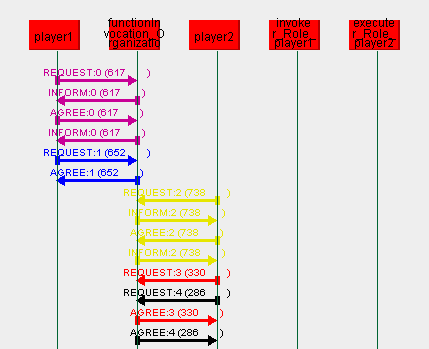
\includegraphics[width=0.8\textwidth]{images/examples/example1-stage1.png}
	\caption{Stage 1: Role enactment}
	\label{figure:example1-stage1}
\end{figure}

% Purple
The \textbf{purple} interaction scenario between \textit{player1} and the \textit{function-invocation} organization follows the \textit{Enact role} protocol.
\textit{player1} requests \textit{invoke-function} to enact the \textit{Invoker} role (1\textsuperscript{st} message) and is informed about the role's responsibilities (2\textsuperscript{nd} message) .
Since \textit{Invoker} has no responsibilities, \textit{player1} agrees that it can indeed enact the role (3\textsuperscript{rd} message).
\textit{invoke-organization} then creates the \textit{invoker-player1} position (modelled by the \texttt{invoker\_Role\_player1} agent instance) and informs \textit{player1} of its AID (4\textsuperscript{th} message).

% Blue
The \textbf{blue} interaction scenario between \textit{player1} and the \textit{function-invocation} organization follows the \textit{Subscribe to event} protocol.
\textit{player1} requests \textit{invoke-function} to subscribe to the \textit{Role activated} event (1\textsuperscript{st} message) and \textit{function-invocation} agrees (2\textsuperscript{nd} message).

% Yellow
The \textbf{yellow} interaction scenario between \textit{player2} and the \textit{invoke-function} organization follows the \textit{Enact role} protocol.
\textit{player2} requests \textit{invoke-function} to enact the \textit{Executer} role (1\textsuperscript{st}) and is informed about the role's responsibilities (2\textsuperscript{nd} message).
Since \textit{player2} can perform one \textit{Executer}'s responsibility -- the \textit{Execute function} responsibility -- it agrees that it can indeed enact the role (3\textsuperscript{rd} message).
\textit{invoke-function} then creates the \textit{executer-player2} position (modelled by the \texttt{executer\_Role\_player2} agent instance) and informs \textit{player2} of its AID (4\textsuperscript{th} message).

% Red
The \textbf{red} interaction scenario between t\textit{player2} and the \textit{function-invocation} organization follows the \textit{Subscribe to event} protocol.
\textit{player2} requests \textit{invoke-function} to subscribe to the \textit{Role activated} event (1\textsuperscript{st} message) and \textit{function-invocation} agrees (2\textsuperscript{nd} message).

% Black
The \textbf{black} interaction scenario between \textit{player2} and the \textit{function-invocation} organization follows the \textit{Subscribe to event} protocol.
\textit{player2} requests \textit{invoke-function} to subscribe to the \textit{Role deactivated} event (1\textsuperscript{st} message) and \textit{function-invocation} agrees (2\textsuperscript{nd} message).

%%%%%%%%%%%%%%%%%%%%%%%%%%%%%%%%%%%%%%%%%%%%%%%%%%%%%%%%%%%%%%%%%%%%%%%%%%%%%%%%
\subsubsection*{Stage 2: Role Activation}

% Figure: Stage 2: Role activation
\begin{figure}[H]
	\centering
	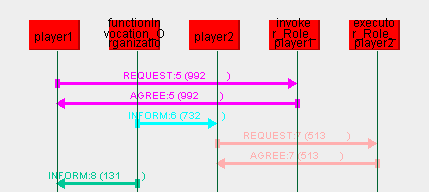
\includegraphics[width=0.8\textwidth]{images/examples/example1-stage2.png}
	\caption{Stage 2: Role activation}
	\label{figure:example1-stage2}
\end{figure}

% Magenta
The \textbf{magenta} interaction scenario between \textit{player1} and the \textit{invoker-player1} position follows the \textit{Activate role} protocol.
\textit{player1} requests \textit{invoker-player1} to activate the role (1\textsuperscript{st} message) and the position promptly agrees (2\textsuperscript{nd} message).

% Cyan
The \textbf{cyan} interaction scenario between the \textit{invoke-function} organization and \textit{player2} follows the \textit{Publish event} protocol.
\textit{invoke-organization} raises a \textit{Role activated} event (for the \textit{Invoker} role) and \textit{player2} handles it by activating its \textit{Executer} role (the \textbf{pink} interaction scenario).

% Pink
The \textbf{pink} interaction scenario between \textit{player2} and the \textit{executer-player2} position follows the \textit{Activate role} protocol.
\textit{player2} requests \textit{executer-player2} to activate the role (1\textsuperscript{st} message) and the position immediately agrees (2\textsuperscript{nd} message).

% Dark green
The \textbf{dark green} interaction scenario between the \textit{invoke-function} organization and \textit{player1} follows the \textit{Publish event} protocol.
\textit{invoke-organization} raises a \textit{Role activated} event (for the \textit{Executer} role) and \textit{player1} handles it by invoking the \textit{Invoke function} competence (the \textbf{light green} interaction scenario).

%%%%%%%%%%%%%%%%%%%%%%%%%%%%%%%%%%%%%%%%%%%%%%%%%%%%%%%%%%%%%%%%%%%%%%%%%%%%%%%%
\subsubsection*{Stage 3: Competence and Responsibility Invocation}

% Figure: Stage 3: Competence and responsibility invocation
\begin{figure}[H]
	\centering
	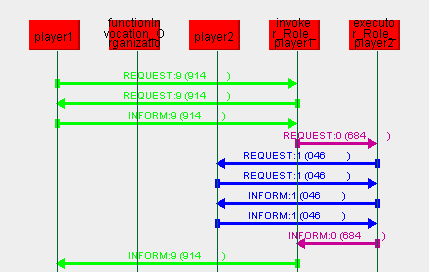
\includegraphics[width=0.8\textwidth]{images/examples/example1-stage3.png}
	\caption{Stage 3: Competence and responsibility invocation}
	\label{figure:example1-stage3}
\end{figure}

% Note - `Invoke competence' protocol vs. 'Invoke function' competence
In the following discussion, is is important to keep in mind that the \textit{Invoke competence} protocol is being used to invoke the \textit{Invoke function} competence.
Understanding the distinction between these two usages of the word `invoke' is a prerequisite to understanding the discussion of Stage 3.

% Light green
The \textbf{light green} interaction scenario between \textit{player1} and the \textit{invoker-player1} position follows the \textit{Invoke competence} protocol.
\textit{player1} requests \textit{invoker-player1} to invoke the \textit{Invoke function} competence (1\textsuperscript{st} message) and is in turn requested to provide the competence argument (2\textsuperscript{nd} message).
\textit{player1} then promptly informs \textit{invoker-player1} about the argument (3\textsuperscript{rd} message).
After \textit{invoker-player1} executes the competence (the \textbf{purple} interaction scenario), it informs \textit{player1} about its result (4\textsuperscript{th} message).

% Purple
The \textbf{purple} interaction scenario between the \textit{initiator-player1} and \textit{executer-player2} positions follows the \textit{Invoke function} protocol.
\textit{initiator-player1} requests \textit{executer-player2} to execute a particular function (factorial) for a particular argument (10, 1\textsuperscript{st} message).
\textit{executer-player2}, after invoking the \textit{Execute function} responsibility on its player (the \textbf{blue} interaction scenario), informs \textit{invoker-player1} about the function return value (3628800, 2\textsuperscript{nd} message).

% Blue
The \textbf{blue} interaction scenario between the \textit{executer-player2} position \textit{player2} follows the \textit{Invoke responsibility} protocol.
\textit{executer-player2} requests \textit{player2} to invoke the \textit{Execute function} responsibility (1\textsuperscript{st} message) and is in turn requested to provide the responsibility argument (2\textsuperscript{nd} message).
\textit{executer-player2} then immediately informs \textit{player2} about the argument (3\textsuperscript{rd} message).
After \textit{player2} executes the responsibility, it informs \textit{executer-player2} about its result (4\textsuperscript{th} message).

%%%%%%%%%%%%%%%%%%%%%%%%%%%%%%%%%%%%%%%%%%%%%%%%%%%%%%%%%%%%%%%%%%%%%%%%%%%%%%%%
\subsubsection*{Stage 4: Role Deactivation}

% Figure: Stage 4: Role deactivation
\begin{figure}[H]
	\centering
	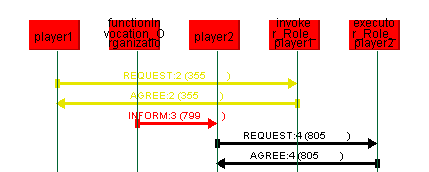
\includegraphics[width=0.8\textwidth]{images/examples/example1-stage4.png}
	\caption{Stage 4: Role deactivation}
	\label{figure:example1-stage4}
\end{figure}

% Yellow
The \textbf{yellow} interaction scenario between \textit{player1}  and the \textit{invoker-player1} position.
\textit{player1} requests \textit{invoker-player1} to deactivate the role (1\textsuperscript{st} message) and the position promptly agrees (2\textsuperscript{nd} message).

% Red
The \textbf{red} interaction scenario between the \textit{invoke-function} organization and \textit{player2} follows the \textit{Publish event} protocol.
\textit{invoke-organization} raises a \textit{Role deactivated} event (for the \textit{Invoker} role) and \textit{player2} handles it by deactivating its \textit{Executer} role (the \textbf{light green} interaction scenario).

% Black
The \textbf{black} interaction scenario between \textit{player2} and the \textit{executer-player2} position.
\textit{player2} requests \textit{executer-player2} to deactivate the role (1\textsuperscript{st} message) and the position immediately agrees (2\textsuperscript{nd} message).

%%%%%%%%%%%%%%%%%%%%%%%%%%%%%%%%%%%%%%%%%%%%%%%%%%%%%%%%%%%%%%%%%%%%%%%%%%%%%%%%
\subsubsection*{Stage 5: Role Deactment}

% Figure: Stage 5: Role deactment
\begin{figure}[H]
	\centering
	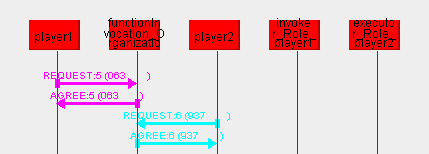
\includegraphics[width=0.8\textwidth]{images/examples/example1-stage5.png}
	\caption{Stage 5: Role deactment}
	\label{figure:example1-stage5}
\end{figure} 

% Magenta
The \textbf{magenta} interaction scenario between \textit{player1} and the \textit{invoke-function} organization.
\textit{player1} requests \textit{invoke-function} to deact the \textit{Invoker} role (1\textsuperscript{st} message) and the organization promptly agrees (2\textsuperscript{nd} message).

% Cyan
The \textbf{cyan} interaction scenario between \textit{player2} and the \textit{invoke-function} organizations.
\textit{player2} requests \textit{invoke-function} to deact the \textit{Executer} role (1\textsuperscript{st} message) and the organization immediately agrees (2\textsuperscript{nd} message).

%%%%%%%%%%%%%%%%%%%%%%%%%%%%%%%%%%%%%%%%%%%%%%%%%%%%%%%%%%%%%%%%%%%%%%%%%%%%%%%%
%% MASTER'S THESIS                                                            %%
%%                                                                            %% 
%% Title (en): Multi-Agent Systems and Organizations                          %%
%% Title (cs): Multiagentní systémy a organizace                              %%
%%                                                                            %%
%% Author: Bc. Lukáš Kúdela                                                   %%
%% Supervisor: Prof. RNDr. Petr Štěpánek, DrSc.                               %%
%%                                                                            %%
%% Academic year: 2011/2012                                                   %%
%%%%%%%%%%%%%%%%%%%%%%%%%%%%%%%%%%%%%%%%%%%%%%%%%%%%%%%%%%%%%%%%%%%%%%%%%%%%%%%%

\section{Example 2: Arithmetic Expression Evaluation}

% Section intro - 'Arithmetic expression evaluation' organziation
This example demonstrates a not-so-simple organization---\textit{arithmetic expression evaluation}.
% 'Arithmetic expression evaluation' - purpose
The purpose of this organization is to facilitate divide-and-conquer evaluation of arithmetic expressions by grouping five agents: one agent \textit{breaks the expression down} (the `divide' part) and the other four compute \textit{addition}, \textit{subtraction}, \textit{multiplication} and \textit{integral division} (the `conquer' part), each agent computing one arithmetic operation.
The reason the organization is formed in the first place is because the agent breaking the expression down is not capable of computing any arithmetic operation itself.
% Assumptions - simple arithmetic expression
In this example, agents evaluate simple arithmetic expressions---consisting of natural numbers, four basic arithmetic operations (addition, subtraction, multiplication and integral division) and parentheses. However, it should be apparent that any arithmetic expressions could be evaluated this way.

%%%%%%%%%%%%%%%%%%%%%%%%%%%%%%%%%%%%%%%%%%%%%%%%%%%%%%%%%%%%%%%%%%%%%%%%%%%%%%%%
\subsection*{Specification}

%%%%%%%%%%%%%%%%%%%%%%%%%%%%%%%%%%%%%%%%%%%%%%%%%%%%%%%%%%%%%%%%%%%%%%%%%%%%%%%%
\subsubsection*{Organization Part}

% 'Expression evaluation' organizaiton type
The \textit{Expression evaluation} organization type (modelled by the \texttt{ExpressionEvaluation\_Organization} agent class) contains five roles---\textit{Evaluator}, \textit{Adder}, \textit{Subtractor}, \textit{Multiplier} and \textit{Divider}---and two protocols---\textit{Evaluate expression} and \textit{Evaluate binary operation}.
% 'expression-evaluation' organization
\textit{Expression evaluation} has one instance in the running MAS: the \textit{expression-evaluation} organization (modelled by the \texttt{expressionEvaluation\_Organization} agent instance).

% 'Evaluator' role
The \textit{Evaluator} role (modelled by the \texttt{Evaluator\_Role} agent class) can evaluate a simple arithmetic expression.
% 'Evaluator' role - multiplicity, competences & responsibilities
The \textit{Evaluator} role is a \textit{multiple} role\footnote{However, only one agent plays the \textit{Evaluator} role in our example.}.
It has one competence---\textit{Evaluate}---and no responsibilities.

% 'Evaluate' competence
The \textit{Evaluate} competence (modelled by the \texttt{Evaluate\_Competence} class) is a competence to evaluate a simple arithmetic expression.
% 'Evaluate' competence - argument & result
It has one argument---an expression (a string)---and one result---the value of this expression (an integer).

% 'Adder' role
The \textit{Adder} role (modelled by the \texttt{Adder\_Role} agent class) can perform addition of two simple arithmetic expressions.
% 'Adder' role - multiplicity, competences & responsibilities
% TODO Consider making the binary operator roles multiple.
The \textit{Adder} role is a \textit{multiple} role\footnote{However, only one agent plays the \textit{Adder} role in our example.}.
It has no competences and one responsibility---\textit{Add}.

% 'Add' responsibility
The \textit{Add} responsibility (modelled by the \texttt{Add\_Responsibility} class) is a responsibility to perform addition of two integers.
% 'Add' responsibility - argument & result
It has two arguments---a pair of addends---and one result---their sum.

% 'Subtractor' role
The \textit{Subtractor} role (modelled by the \texttt{Subtractor\_Role} agent class) can perform subtraction of two simple arithmetic expressions.
% 'Subtractor' role - multiplicity, competences & responsibilities
The \textit{Subtractor} role is a \textit{multiple} role\footnote{However, only one agent plays the \textit{Subtractor} role in our example.}.
It has no competences and one responsibility---\textit{Subtract}.

% 'Subtract' responsibility
The \textit{Subtract} responsibility (modelled by the \texttt{Subtract\_Responsibility} class) is a responsibility to perform subtraction of two integers.
% 'Subtract' responsibility - argument & result
It has two arguments---a minuend and a subtrahend---and one result---their difference.

% 'Multiplier' role
The \textit{Multiplier} role (modelled by the \texttt{Multiplier\_Role} agent class) can perform multiplication of two simple arithmetic expressions.
% 'Multiplier' role - multiplicity, competences & responsibilities
The \textit{Multiplier} role is a \textit{multiple} role\footnote{However, only one agent plays the \textit{Multiplier} role in our example.}.
It has no competences and one responsibility---\textit{Multiply}.

% 'Multiply' responsibility
The \textit{Multiply} responsibility (modelled by the \texttt{Multiply\_Responsibility} class) is a responsibility to perform multiplication of two integers.
% 'Multiply' responsibility - argument & result
It has two arguments---a pair of factors---and one result---their product.

% 'Divider' role
The \textit{Divider} role (modelled by the \texttt{Divider\_Role} agent class) can perform division of two simple arithmetic expressions.
% 'Divider' role - multiplicity, competences & responsibilities
The \textit{Divider} role is a \textit{multiple} role\footnote{However, only one agent plays the \textit{Divider} role in our example.}.
It has no competences and one responsibility---\textit{Divide}.

% 'Divide' responsibility
The \textit{Divide} responsibility (modelled by the \texttt{Divide\_Responsibility} class) is a responsibility to perform integral division of two integers.
% 'Multiply' responsibility - argument & result
It has two arguments---a dividend and a divisor---and one result---their quotient.

% 'Binary operator' role
In the following, we will use the \textit{Binary operator} abstract role to refer to refer to the \textit{Adder}, \textit{Subtractor}, \textit{Multiplier} or \textit{Divisor} role where it is not necessary to distinguish between them.

%%%%%%%%%%%%%%%%%%%%%%%%%%%%%%%%%%%%%%%%%%%%%%%%%%%%%%%%%%%%%%%%%%%%%%%%%%%%%%%%
\subsubsection*{Protocol Part}

% 'Evaluate expresion' protocol
The \textit{Evaluate expression} protocol (modelled by the \texttt{EvaluateExpressionProtocol} class) is a protocol by which a \textit{Binary operator} (the initiator party, modelled by the \texttt{EvaluateExpression\_InitiatorParty}) requests an \textit{Evaluator} (the responder party, modelled by the \texttt{EvaluateExpression\_ResponderParty}) to evaluate an expression.

% 'Evaluate expression request' message
The \textit{Evaluate expression request} message (modelled by the \texttt{EvaluateExpressionRequestMessage} class) is a message sent by a \textit{Binary operator} to an \textit{Evaluator} requesting the latter to evaluate an expression.

% 'Evalaute expression reply' message
The \textit{Evaluate expression reply} message (modelled by the \texttt{EvaluateExpressionReplyMessage} class) is a message sent by an \textit{Evaluator} to a \textit{Binary operator} informing the latter about the value of the evaluated expression.

% 'Evaluate binary operation' protocol
The \textit{Evaluate binary operation} protocol (modelled by the \texttt{EvaluateBinaryOperationProtocol} class) is a protocol by which an \textit{Evaluator} (the initiator party, modelled by the \texttt{EvaluateBinaryOperation\_InitiatorParty}) requests a \textit{Binary operator} (the responder party, modelled by the \texttt{EvaluateBinaryOperation\_ResponderParty}) to evaluate a binary operation.

% 'Evalaute binary operation request' message
The \textit{Evaluate binary operation request} message (modelled by the \texttt{EvaluateBinaryOperationReqestMessage} class) is a message sent by a \textit{Evaluator} to a \textit{Binary Operator} requesting the latter to evaluate a binary operation between two operand expressions.

% 'Evaluate binary operation reply' message
The \textit{Evaluate binary operation reply} message (modelled by the \texttt{EvaluateBinaryOperationReplyMessage} class) is a message sent by a \textit{Binary operator} to an \textit{Evaluator} informing the latter about the value of the evaluated binary operation.

%%%%%%%%%%%%%%%%%%%%%%%%%%%%%%%%%%%%%%%%%%%%%%%%%%%%%%%%%%%%%%%%%%%%%%%%%%%%%%%%
\subsubsection*{Player Part}

% 'Blank' player type
The \textit{Blank} player type (modelled by the \texttt{Blank\_Player} agent class) is a player with no capabilities.
It has one instance in the running MAS: \textit{player1}.
% 'player1' player
\textit{player1} (modelled by the \texttt{player1} agent instance) intends to enact the \textit{Evaluator} role in the \textit{expression-evaluation} organization and to exercise the role's \textit{Evaluate} competence---to have an expression evaluated by the players of the \textit{Binary operator} roles.

% 'Addition computer' player type
The \textit{Addition computer} player type (modelled by the \texttt{AdditionComputer\_Player} agent class) is a player capable of computing the addition operation.
It has one instance in the running MAS: \textit{player2}.
% 'player2' player
\textit{player2} (modelled by the \texttt{player2} agent instance) intends to enact the \textit{Adder} role in the \textit{expression-evaluation} organization and fulfil the role's \textit{Add} responsibility---to compute addition during the evaluation of the expression from the player of the \textit{Evaluator} role.

% 'Subtraction computer' player type
The \textit{Subtraction computer} player type (modelled by the \texttt{SubtractionComputer\_Player} agent class) is a player capable of computing the subtraction operation.
It has one instance in the running MAS: \textit{player3}.
% 'player3' player
The intention of \textit{player3} (modelled by the \texttt{player3} agent instance) is to enact the \textit{Subtractor} role in the \textbf{expression-evaluation} organization and perform the role's \textit{Subtract} responsibility---to compute subtraction during the evaluation of the expression from the player of the  \textit{Evaluator} role.

% 'Multiplication computer' player type
The \textit{Multiplication computer} player type (modelled by the \texttt{MultiplicationComputer\_Player} agent class) is a player capable of computing the multiplication operation.
It has one instance in the running MAS: \textit{player4}.
% 'player4' player
\textit{player4} (modelled by the \texttt{player4} agent instance) intends to enact the \textit{Multiplier} role in the \textit{expression-evaluation} organization and fulfil the role's \textit{Multiply} responsibility---to compute multiplication during the evaluation of the expression from the player of the \textit{Evaluator} role.

% 'Division computer' player type
The \textit{Division computer} player type (modelled by the \texttt{DivisionComputer\_Player} agent class) is a player capable of computing the division operation.
It has one instance in the running MAS: \textit{player5}.
% 'player5' player
The intention of \textit{player5} (modelled by the \texttt{player5} agent instance) is to enact the \textit{Divisor} role in the \textit{expression-evaluation} organization and fulfil the role's \textit{Divide} responsibility---to compute division during the evaluation of the expression from the player of the \textit{Evaluator} role.

%%%%%%%%%%%%%%%%%%%%%%%%%%%%%%%%%%%%%%%%%%%%%%%%%%%%%%%%%%%%%%%%%%%%%%%%%%%%%%%%
\subsection*{Manifestation}

%%%%%%%%%%%%%%%%%%%%%%%%%%%%%%%%%%%%%%%%%%%%%%%%%%%%%%%%%%%%%%%%%%%%%%%%%%%%%%%%
\subsubsection*{Stage 1: Role Enactment}

% Figure: Stage 1: Role enactment
\begin{figure}[H]
	\centering
	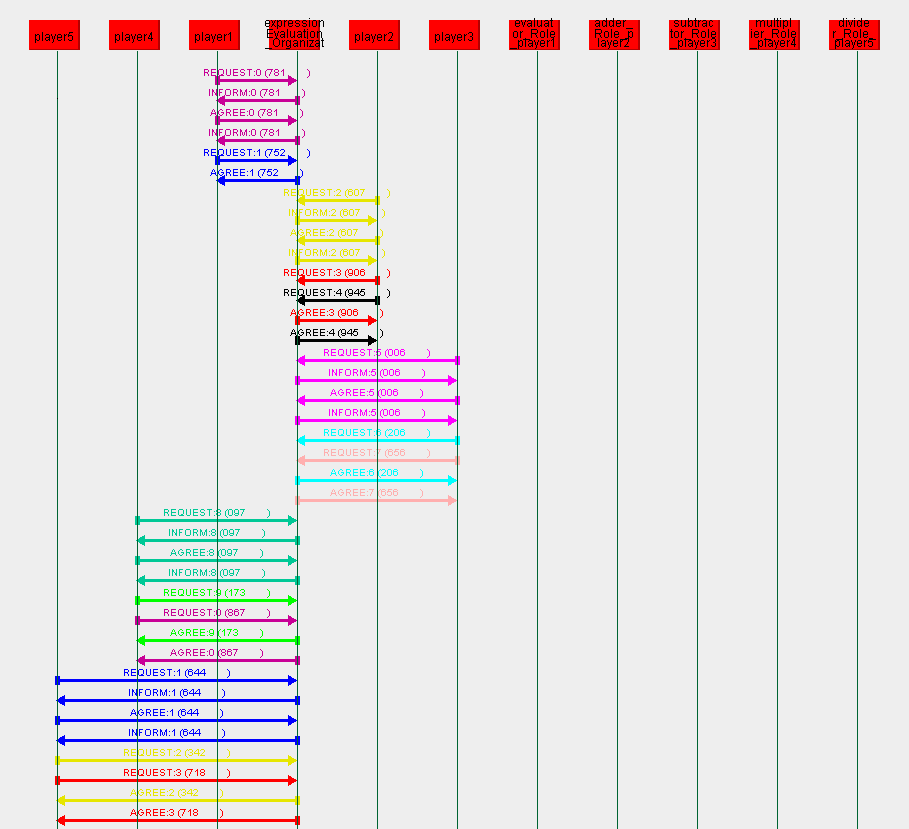
\includegraphics[width=\textwidth]{images/examples/example2-stage1.png}
	\caption{Stage 1: Role enactment}
	\label{figure:example2-stage1}
\end{figure}

% First purple
In the {\color{purple}{\textbf{first purple}}} interaction scenario, \textit{player1} enacts the \textit{Evaluator} role, resulting in the creation of the \textit{evaluator-player1} position.
% First blue
In the {\color{blue}{\textbf{first blue}}} interaction scenario, \textit{player1} subscribes to the \textit{Activate role} event.

% First yellow
In the {\color{yellow}{\textbf{first yellow}}} interaction scenario, \textit{player2} enacts the \textit{Adder} role, resulting in the creation of the \textit{adder-player2} position.
% First red & Black
In the {\color{red}{\textbf{first red}}} and {\color{black}{\textbf{black}}} interaction scenarios, \textit{player2} subscribes to the \textit{Activate role} and \textit{Deactivate role} events respectively.

% Magenta
In the {\color{magenta}{\textbf{magenta}}} interaction scenario, \textit{player3} enacts the \textit{Subtractor} role, resulting in the creation of the \textit{subtractor-player3} position.
% Cyan & Pink
In the {\color{cyan}{\textbf{cyan}}} and {\color{pink}{\textbf{pink}}} interaction scenarios, \textit{player3} subscribes to the \textit{Activate role} and \textit{Deactivate role} events respectively.

% Teal
In the {\color{teal}{\textbf{teal}}} interaction scenario, \textit{player4} enacts the \textit{Multiplier} role, resulting in the creation of the \textit{multiplier-player4} position.
% Green & Second purple
In the {\color{green}{\textbf{green}}} and {\color{purple}{\textbf{second purple}}} interaction scenarios, \textit{player4} subscribes to the \textit{Activate role} and \textit{Deactivate role} events respectively.

% Second blue
In the {\color{blue}{\textbf{second blue}}} interaction scenario, \textit{player5} enacts the \textit{Divider} role, resulting in the creation of the \textit{divider-player5} position.
% Second yellow & Second red
In the {\color{yellow}{\textbf{second yellow}}} and {\color{red}{\textbf{second red}}} interaction scenarios, \textit{player5} subscribes to the \textit{Activate role} and \textit{Deactivate role} events respectively.

%%%%%%%%%%%%%%%%%%%%%%%%%%%%%%%%%%%%%%%%%%%%%%%%%%%%%%%%%%%%%%%%%%%%%%%%%%%%%%%%
\subsubsection*{Stage 2: Role Activation}

% Figure: Stage 2: Role activation
\begin{figure}[H]
	\centering
	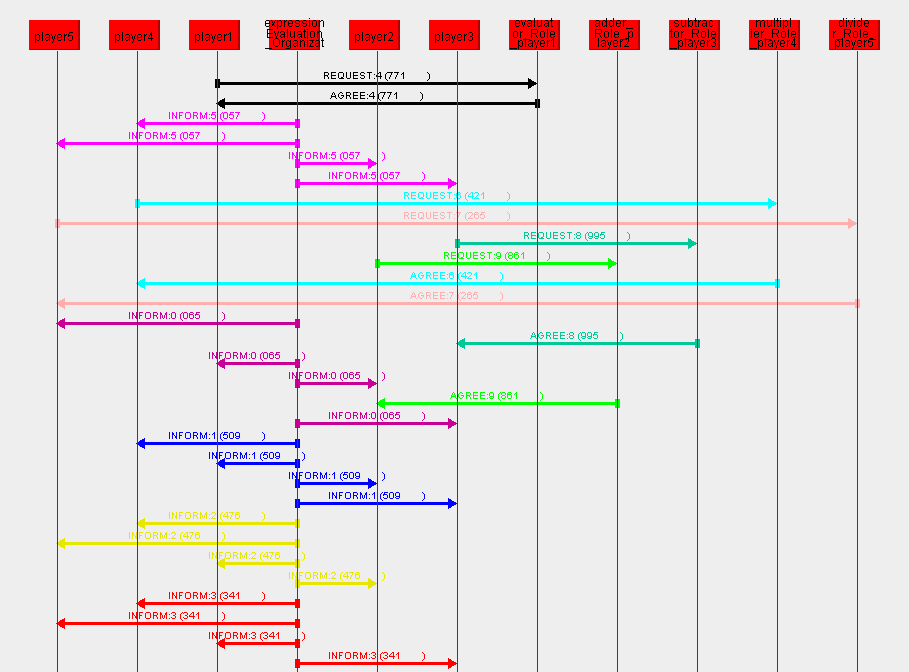
\includegraphics[width=\textwidth]{images/examples/example2-stage2.png}
	\caption{Stage 2: Role activation}
	\label{figure:example2-stage2}
\end{figure}

% Black
In the {\color{black}{\textbf{black}}} interaction scenario, \textit{player1} activates its \textit{Evaluator} role.
% Magenta
In the {\color{magenta}{\textbf{magenta}}} interaction scenario, the \textit{expression-evaluation} organization publishes the \textit{Role activated} event (for the \textit{Eveluator} role).
\textit{player2} reacts by activating its \textit{Adder} role (the {\color{green}{\textbf{green}}} interaction scenario), \textit{player3} by activating its \textit{Subtractor} role (the {\color{teal}{\textbf{teal}}} interaction scenario), \textit{player4} by activating its \textit{Multiplier} role (the {\color{cyan}{\textbf{cyan}}} interaction scenario) and \textit{player5} by activating its \textit{Divider} role (the {\color{pink}{\textbf{pink}}} interaction scenario).

% Green
In the {\color{green}{\textbf{green}}} interaction scenario, \textit{player2} activates its \textit{Adder} role.
% Red
In the {\color{red}{\textbf{red}}} interaction scenario, the \textit{expression-evaluation} organization publishes the \textit{Role activated} event (for the \textit{Adder} role).

% Teal
In the {\color{teal}{\textbf{teal}}} interaction scenario, \textit{player3} activates its \textit{Subtractor} role.
% Yellow
In the {\color{yellow}{\textbf{yellow}}} interaction scenario, the \textit{expression-evaluation} organization publishes the \textit{Role activated} event (for the \textit{Subtractor} role).

% Cyan
In the {\color{cyan}{\textbf{cyan}}} interaction scenario, \textit{player4} activates its \textit{Multiplier} role.
% Purple
In the {\color{purple}{\textbf{purple}}} interaction scenario, the \textit{expression-evaluation} organization publishes the \textit{Role activated} event (for the \textit{Multiplier} role).

% Pink
In the {\color{pink}{\textbf{pink}}} interaction scenario, \textit{player5} activates its \textit{Divider} role.
% Blue
In the {\color{blue}{\textbf{blue}}} interaction scenario, the \textit{expression-evaluation} organization publishes the \textit{Role activated} event (for the \textit{Divider} role).

% Event originator not notified
Note that that in all role activation scenarios, the player activating a role is not notified about the resulting \textit{Role activated} event, although it is subscribed to it; there is no need to notify the player causing the event in the first place.

%%%%%%%%%%%%%%%%%%%%%%%%%%%%%%%%%%%%%%%%%%%%%%%%%%%%%%%%%%%%%%%%%%%%%%%%%%%%%%%%
\subsubsection*{Stage 3: Competence and Responsibility Invocation}

% Figure: Stage 3: Competence and responsiility invocation
\begin{figure}[H]
	\centering
	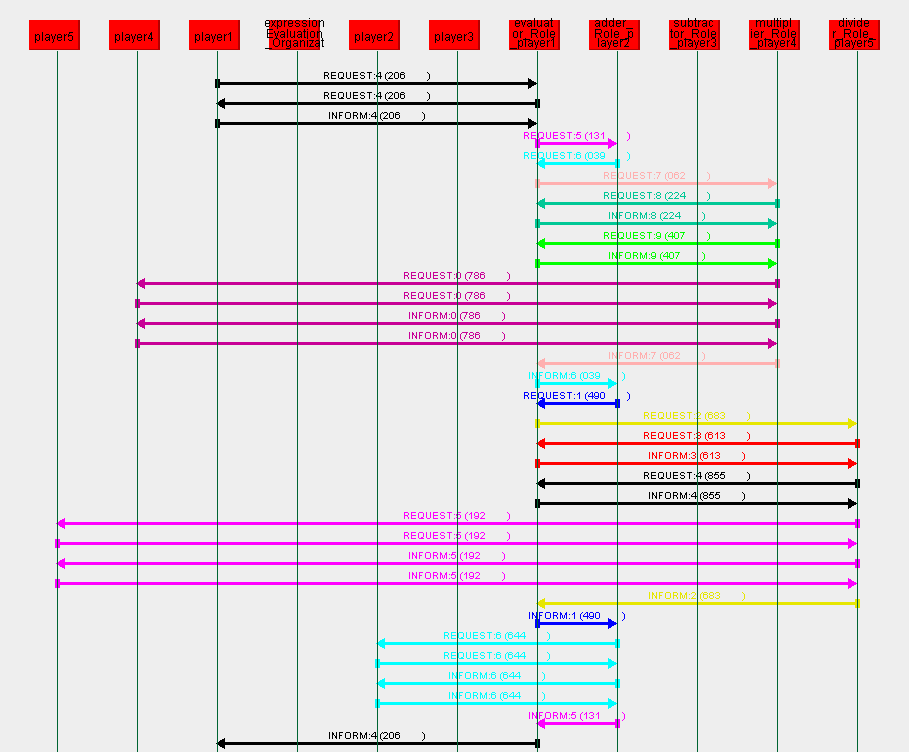
\includegraphics[width=\textwidth]{images/examples/example2-stage3.png}
	\caption{Stage 3: Competence and responsibility invocation}
	\label{figure:example2-stage3}
\end{figure}

The \textit{Evaluate expression} competence is invoked by \textit{player1} on its \textit{Evaluator} role and is carried out in a divide-and-conquer fashion by an \textit{Evaluator}, an \textit{Adder}, a \textit{Multiplier} and a \textit{Divider} by collaborating with one another and invoking responsibilities on their respective players.
In this example the arithmetic expression to be evaluated is $(1\cdot2)+(4/2)$.

% Evaluator: "(1*2)+(4/2)"
In the {\color{black}{\textbf{first black}}} interaction scenario, the \textit{evaluator-player1} position is requested by \textit{player1} to invoke the \textit{Evaluate} competence for the expression $(1\cdot2)+(4/2)$.
First, it parses the expression, finds the operation to be applied last---addition---and splits the expression into two sub-expressions to be added.
Next, it requests \textit{adder-player2} to evaluate their sum (the {\color{magenta}{\textbf{first magenta}}} interaction scenario).
Finally, it reports the value (4) to \textit{player1}.

% Adder: "(1*2)", "(4/2)"
In the {\color{magenta}{\textbf{first magenta}}} interaction scenario, the \textit{adder-player2} position is requested to evaluate the sum of the expressions $(1\cdot2)$ and $(4/2)$.
First, it requests \textit{evaluator-player1} to evaluate both expressions (the {\color{cyan}{\textbf{first cyan}}} and {\color{blue}{\textbf{blue}}} interaction scenarios).
Next, it invokes the \textit{Add} responsibility on \textit{player2} to calculate the sum of their values (the {\color{cyan}{\textbf{second cyan}}} interaction scenario).
Finally, it reports the sum (4) to \textit{evaluator-player1} (the original {\color{magenta}{\textbf{first magenta}}} interaction scenario).

% Evaluator: "(1*2)"
In the {\color{cyan}{\textbf{first cyan}}} interaction scenario, the \textit{evaluator-player1} position is requested to evaluate the expression $(1\cdot2)$.
First, it parses the expression, finds the last-to-be-applied operation---multiplication---and splits the expression into two sub-expressions to be multiplied.
Next, it requests \textit{multiplier-player4} to evaluate their product (the {\color{pink}{\textbf{pink}}} interaction scenario).
Finally, it reports the value (2) to \textit{adder-player2}.

% Multiplier: "1", "2"
In the {\color{pink}{\textbf{pink}}} interaction scenario, the \textit{multiplier-player4} position is requested to evaluate the product of the expressions $1$ and $2$.
First, it requests \textit{evaluator-player1} to evaluate both expressions (the {\color{teal}{\textbf{teal}}} and {\color{green}{\textbf{green}}} interaction scenarios).
Next, it invokes the \textit{Multiply} responsibility on \textit{player4} to calculate the product of their values (the {\color{purple}{\textbf{purple}}} interaction scenario).
Finally, it reports the product (2) to \textit{evaluator-player1} (the original {\color{pink}{\textbf{pink}}} interaction scenario).

% Evaluator: "1"
In {\color{teal}{\textbf{teal}}} interaction scenario, the \textit{evaluator-player1} is requested to evaluate the expression $1$.
It parses the expression, finds out it is a number (bottom case) and reports the value (1) to \textit{multiplier-player4}.

% Evaluator: "2"
In {\color{green}{\textbf{green}}} interaction scenario, the \textit{evaluator-player1} is requested to evaluate the expression $2$.
It parses the expression, finds out it is a number (bottom case) and reports the value (2) to \textit{multiplier-player4}.

% Evaluator: "(4/2)"
In the {\color{blue}{\textbf{blue}}} interaction scenario, the \textit{evaluator-player1} is requested to evaluate the expression $(4/2)$.
First, it parses the expression, finds the last-to-be-applied operation---division---and splits the expression into two sub-expressions to be divided.
Next, it requests \textit{divider-player5} to evaluate their product (the {\color{yellow}{\textbf{yellow}}} interaction scenario).
Finally, it reports the value (2) to \textit{adder-player2}.

% Divider: "4", "2"
In the {\color{yellow}{\textbf{yellow}}} interaction scenario, the \textit{divider-player5} position is requested to evaluate the quotient of the expressions $4$ and $2$.
First, it requests \textit{evaluator-player1} to evaluate both expressions (the {\color{red}{\textbf{red}}} and {\color{black}{\textbf{black}}} interaction scenarios).
Next, it invokes the \textit{Divide} responsibility on \textit{player5} to calculate the quotient of their values (the {\color{magenta}{\textbf{second magenta}}} interaction scenario).
Finally, it reports the quotient (2) to \textit{evaluator-player1} (the original {\color{yellow}{\textbf{yellow}}} interaction scenario).

% Evaluator: "4"
In {\color{red}{\textbf{red}}} interaction scenario, the \textit{evaluator-player1} is requested to evaluate the expression $4$.
It parses the expression, finds out it is a number (bottom case) and reports the value (4) to \textit{divider-player5}.

% Evaluator: "2"
In {\color{black}{\textbf{black}}} interaction scenario, the \textit{evaluator-player1} is requested to evaluate the expression $2$.
It parses the expression, finds out it is a number (bottom case) and reports the value (2) to \textit{divider-player5}.

%%%%%%%%%%%%%%%%%%%%%%%%%%%%%%%%%%%%%%%%%%%%%%%%%%%%%%%%%%%%%%%%%%%%%%%%%%%%%%%%
\subsubsection*{Stage 4: Role Deactivation}

% Figure: Stage 4: Role deactivation
\begin{figure}[H]
	\centering
	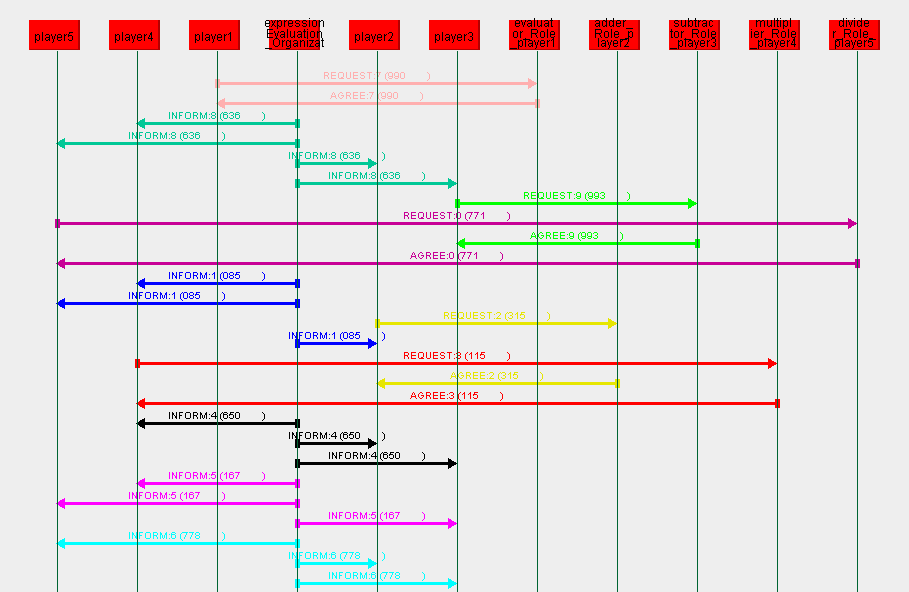
\includegraphics[width=\textwidth]{images/examples/example2-stage4.png}
	\caption{Stage 4: Role deactivation}
	\label{figure:example2-stage4}
\end{figure}

% Pink
In the {\color{pink}{\textbf{pink}}} interaction scenario, \textit{player1} deactivates its \textit{Evaluator} role.
% Teal
In the {\color{teal}{\textbf{teal}}} interaction scenario, the \textit{expression-evaluation} organization publishes the \textit{Role deactivated} event (for the \textit{Evaluator} role).
\textit{player2} reacts by deactivating its \textit{Adder} role (the {\color{yellow}{\textbf{yellow}}} interaction scenario), \textit{player3} by deactivating its \textit{Subtractor} role (the {\color{green}{\textbf{green}}} interaction scenario), \textit{player4} by deactivating its \textit{Multiplier} role (the {\color{red}{\textbf{red}}} interaction scenario) and \textit{player5} by deactivating its \textit{Divider} role (the {\color{purple}{\textbf{purple}}} interaction scenario).

% Yellow
In the {\color{yellow}{\textbf{yellow}}} interaction scenario, \textit{player2} deactivates its \textit{Adder} role.
% Magenta
In the {\color{magenta}{\textbf{magenta}}} interaction scenario, the \textit{expression-evaluation} organization publishes the \textit{Role deactivated} event (for the \textit{Adder} role).

% Green
In the {\color{green}{\textbf{green}}} interaction scenario, \textit{player3} deactivates its \textit{Subtractor} role.
% Blue
In the {\color{blue}{\textbf{blue}}} interaction scenario, the \textit{expression-evaluation} organization publishes the \textit{Role deactivated} event (for the \textit{Subtractor} role).

% Red
In the {\color{red}{\textbf{red}}} interaction scenario, \textit{player4} deactivates its \textit{Multiplier} role.
% Cyan
In the {\color{cyan}{\textbf{cyan}}} interaction scenario, the \textit{expression-evaluation} organization publishes the \textit{Role deactivated} event (for the \textit{Multiplier} role).

% Purple
In the {\color{purple}{\textbf{purple}}} interaction scenario, \textit{player5} deactivates its \textit{Divider} role.
% Black
In the {\color{black}{\textbf{black}}} interaction scenario, the \textit{expression-evaluation} organization publishes the \textit{Role deactivated} event (for the \textit{Divider} role).

%%%%%%%%%%%%%%%%%%%%%%%%%%%%%%%%%%%%%%%%%%%%%%%%%%%%%%%%%%%%%%%%%%%%%%%%%%%%%%%%
\subsubsection*{Stage 5: Role Deactment}

% Figure: Stage 5: Role deactment
\begin{figure}[H]
	\centering
	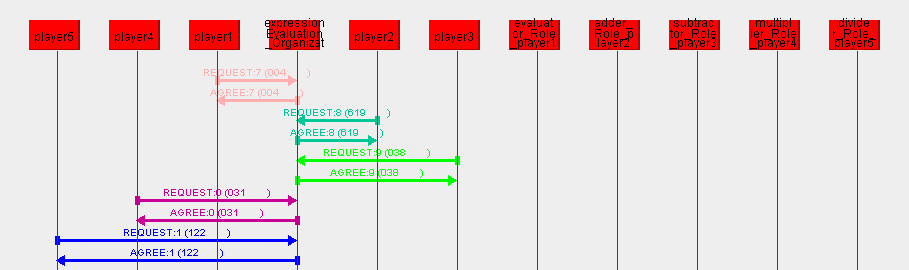
\includegraphics[width=\textwidth]{images/examples/example2-stage5.png}
	\caption{Stage 5: Role deactment}
	\label{figure:example2-stage5}
\end{figure} 

% Pink
In the {\color{pink}{\textbf{pink}}} interaction scenario, \textit{player1} deacts its \textit{Evaluator} role and the \textit{evaluator-player1} position is abolished.

% Teal
In the {\color{teal}{\textbf{teal}}} interaction scenario, \textit{player2} deacts its \textit{Adder} role and the \textit{adder-player2} position is abolished.

% Green
In the {\color{green}{\textbf{green}}} interaction scenario, \textit{player3} deacts its \textit{Subtractor} role and the \textit{subtractor-player3} position is abolished.

% Purple
In the {\color{purple}{\textbf{purple}}} interaction scenario, \textit{player4} deacts its \textit{Multiplier} role and the \textit{multiplier-player4} position is abolished.

% Blue
In the {\color{blue}{\textbf{blue}}} interaction scenario, \textit{player5} deacts its \textit{Divider} role and the \textit{divider-player5} position is abolished.

%%%%%%%%%%%%%%%%%%%%%%%%%%%%%%%%%%%%%%%%%%%%%%%%%%%%%%%%%%%%%%%%%%%%%%%%%%%%%%%%
%% Title (en): Multiagent Systems and Organizations                           %%
%% Title (cs): Multiagentní systémy a organizace                              %%
%%                                                                            %%
%% Author: Bc. Lukáš Kúdela                                                   %%
%% Supervisor: Prof. RNDr. Petr Štěpánek, DrSc.                               %%
%%                                                                            %%
%% Academic year: 2011/2012                                                   %%
%%%%%%%%%%%%%%%%%%%%%%%%%%%%%%%%%%%%%%%%%%%%%%%%%%%%%%%%%%%%%%%%%%%%%%%%%%%%%%%%

%%%%%%%%%%%%%%%%%%%%%%%%%%%%%%%%%%%%%%%%%%%%%%%%%%%%%%%%%%%%%%%%%%%%%%%%%%%%%%%%
\section{Example 3: Auction}
%%%%%%%%%%%%%%%%%%%%%%%%%%%%%%%%%%%%%%%%%%%%%%%%%%%%%%%%%%%%%%%%%%%%%%%%%%%%%%%%

% Auction organization
This example demonstrates a relatively complex organization - the auction.
% Auction organization - purpose
The purpose of this organization is to facilitate auction by bringing together several agents: one agent auctions an item and the other agents bid for it.
The item can be auctioned in an envelope, Vickrey, english or dutch auction.
% Assumptions
In this example, agents sell and buy works of art (famous paintings) in an envelope auction, but it should be obvious that any of the four auction types could be used to sell any items.

%%%%%%%%%%%%%%%%%%%%%%%%%%%%%%%%%%%%%%%%%%%%%%%%%%%%%%%%%%%%%%%%%%%%%%%%%%%%%%%%
\subsection*{Specification}

%%%%%%%%%%%%%%%%%%%%%%%%%%%%%%%%%%%%%%%%%%%%%%%%%%%%%%%%%%%%%%%%%%%%%%%%%%%%%%%%
\subsubsection*{Organization Part}

% 'Auction' organizaiton type
The \textit{Auciton} organization type (modelled by the \texttt{Auction\_Organization} agent class) contains two roles - \textit{Auctioneer} and \textit{Bider} - and four protocols - \textit{Envelope auction}, \textit{Vickrey auction}, \textit{English auction} and \textit{Dutch auction}.
% 'auction' organization
\textit{Auction} has one instance in the running MAS - the \textit{auction} organization (modelled by the \texttt{auction\_Organization} agent instance).

% 'Auctioneer' role
The \textit{Auctioneer} role (modelled by the \texttt{Auctioneer\_Role} class) can sell an item in an auction, i.e. it can auction an item.
% 'Auctioneer' role - multiplicity, competences & responsibilities
The \textit{Auctioneer} role is a \textit{single} role.
It has one competence - \textit{Auction} - and no responsibilities.

% 'Auction' competence
The \textit{Auction} competence (modelled by the \texttt{Auction\_Competence} class) is a competence to auction an item.
% 'Auction' competence - argument & result
It has several arguments depending on the type of the auction - mainly the name of the item - and several results - particularly the hammer price.

% 'Bidder' role
The \textit{Bidder} role (modelled by the \texttt{Bidder\_Role} class) can buy an item in an auction, i.e. it can bid for an item. 
% 'Bidder' role - multiplicity, competences & responsibilities
The \textit{Bidder} role is a \textit{multiple} role.
It has no competences and one responsibility - \textit{Bid}.

% 'Bid' responsibility
The \textit{Bid} responsibility (modelled by the \texttt{Bid\_Responsibility} class) is a responsibility to bid for an item.
% 'Bid' responsibility - argument & result
It has several arguments depending on the type of the auction - mainly the name of the item - and several results - the bid in particular.

%%%%%%%%%%%%%%%%%%%%%%%%%%%%%%%%%%%%%%%%%%%%%%%%%%%%%%%%%%%%%%%%%%%%%%%%%%%%%%%%
\subsubsection*{Protocol Part}

% 'Envelope acution' protocol
The \textit{Envelope auction} protocol (modelled by the \texttt{EnvelopeAuctionProtocol} class) is a protocol through which an \textit{Auctioneer} (the initiator party, modelled by the \texttt{EnvelopeAuction\_InitiatorParty} class) can determine the best buyer from among the \textit{Bidders} (responder party, modelled by the \texttt{EnvelopeAuction\_RespoderParty} class).
% Envelope auction
The Envelope auction is a sealed bid first-price auction.
In this type of auction the sealed bids (unknown to other bidders) are submitted simultaneously to the auctioneer and the item is sold to the winning bidder for the price of their bid.

% Vickrey auction protocol
The \textit{Vickrey auction} protocol (modelled by the \texttt{VickreyAuctionProtocol} class) is a protocol through which an \textit{Auctioneer} (the initiator party, modelled by the \texttt{VickreyAuction\_InitiatorParty} class) can choose the best buyer from among the \textit{Bidders} (responder party, modelled by the \texttt{VickreyAuction\_RespoderParty} class).
% Vickrey auction
The Vickrey auction is a sealed bid second-price auction.
In this type of auction the sealed bids are submitted simultaneously to the auctioneer and the item is sold to the winning bidder for the price of the \textit{second} highest bid.

% English auction protocol
The \textit{English auction} protocol (modelled by the \texttt{EnglishAuctionProtocol} class) is a protocol through which an \textit{Auctioneer} (the initiator party, modelled by the \texttt{EnglishAuction\_InitiatorParty} class) can determine the best buyer from among the \textit{Bidders} (responder party, modelled by the \texttt{EnglishAuction\_RespoderParty} class).
% English auction
The English auction is an open bid ascending price auction.
In this type of auction the auctioneer announces the starting price (lower than the expected selling price).
The bidders then sequentially submit open bids in ascending fashion, respecting the minimum increment.
The item is sold to the \textit{last} bidder willing to pay the price.

% Dutch auction protocol
The \textit{Dutch auction} protocol (modelled by the \texttt{DutchAuctionProtocol} class) is a protocol through which an \textit{Auctioneer} (the initiator party, modelled by the \texttt{DutchAuction\_InitiatorParty} class) can determine the best buyer from among the \textit{Bidders} (responder party, modelled by the \texttt{DutchAuction\_RespoderParty} class).
% Dutch auction
The Dutch auction is an open bid descending price auction.
In this type of auction the auctioneer announces a starting price (higher than the expected selling price).
The auctioneer then sequentially offers prices in descending fashion, respecting the minimum decrement.
The item is sold to the \textit{first} bidder willing to pay the price.

% 'Auction call-for-proposals' message
The \textit{Auction call-for-proposals (CFP)} message (modelled by the \texttt{AuctionCFPMessage} class) is a message sent by an \textit{Auctioneer} to all \textit{Bidders} calling for proposals for the auctioned item's price.

% 'Bid propose' message
The \textit{Bid propose} message (modelled by the \texttt{BidProposeMessage} class) is a message sent by a \textit{Bidder} to an \textit{Auctioneer} proposing a bid to the latter.

%%%%%%%%%%%%%%%%%%%%%%%%%%%%%%%%%%%%%%%%%%%%%%%%%%%%%%%%%%%%%%%%%%%%%%%%%%%%%%%%
\subsubsection*{Player Part}

% 'Participant' player type
The \textit{Participant} player type (modelled by the \texttt{Participant} agent class) is a player capable of biding for an item.
\textit{Participant} has three instances in the running MAS - \textit{player1}, \textit{player2} and \textit{player3}.
All of them intend to enact both the \textit{Auctioneer} and \textit{Bidder} roles in the \textit{auction} organization and perform the \textit{Auctioneer} role's \textit{Auction} competence - to auction an item to the players of the \textbf{Bidder} role.
They also intend to perform the \textit{Bidder} role's \textit{Bid} responsibility - to bid for an item auctioned by the player of the \textit{Auctioneer} role.
% 'player1' player
\textit{player1} (modelled by the \texttt{player1} agent instance) intends to play the \textbf{Auctioneer} in the first round and be the \textbf{Bidder} in the second and third rounds.
% 'player2' player
\textit{player2} (modelled by the \texttt{player2} agent instance) intends to be the \textit{Auctioneer} in the second round and play the \textit{Bidder} in the first and third rounds.
% 'player3' player
\textit{player3} (modelled by the \texttt{player3} agent instance) intends to play the \textit{Auctioneer} in the third rounds and be the \textit{Bidder} in the first and second rounds.

%%%%%%%%%%%%%%%%%%%%%%%%%%%%%%%%%%%%%%%%%%%%%%%%%%%%%%%%%%%%%%%%%%%%%%%%%%%%%%%%
\section{Manifestation} 

%%%%%%%%%%%%%%%%%%%%%%%%%%%%%%%%%%%%%%%%%%%%%%%%%%%%%%%%%%%%%%%%%%%%%%%%%%%%%%%%
\subsubsection*{Stage 3: Competence and Responsibility Invocation}

% Figure: Stage 3: Competence and responsibility invocation
\begin{figure}[H]
	\centering
	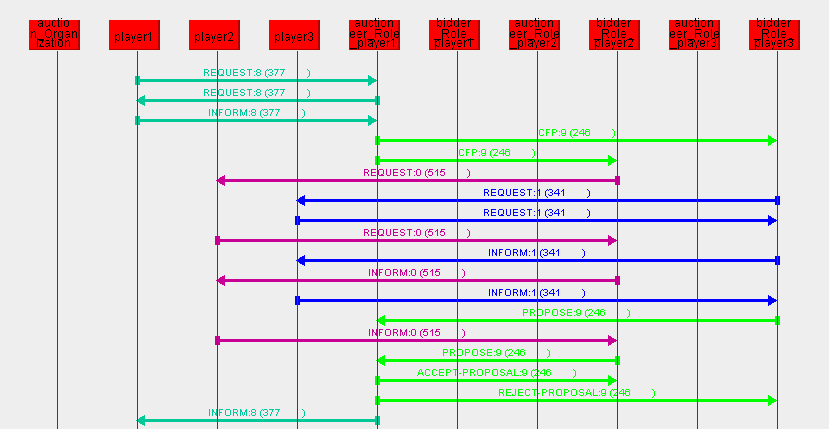
\includegraphics[width=\textwidth]{images/examples/example3-stageA3.png}
	\caption{Stage 3: Competence and responsibility invocation}
	\label{figure:example3-stageA3}
\end{figure}

First, \textit{player1} invokes the \textit{Auction} competence from its \textit{auctioneer-player1} position with parameters of the auction - the name of the item and the reservation price (the \textbf{dark green} interaction scenario).
\textit{auctioneer-player1} calls for proposals for the item price from all \textit{Bidder} positions (the \textbf{light green} interaction scenario).
To come up with their bids, the \textit{bidder-player2} and \textit{bidder-player3} invoke the \textit{Bid} responsibilities from \textit{player2} and \textit{player3} respectively (the \textbf{purple} and \textbf{blue} interaction scenarios respectively).
\textit{bidder-player2} and \textit{bidder-player3} propose their bids to \textit{auctioneer-player1} who determines if the auction is successful or not, i. e. whether the auction winner has been found.
If the highest bid is at least as high as the reservation price, the auction is successful, the winner is the highest bidding bidder and the hammer price is their bid; otherwise, the auction is unsuccessful.
Next, \textit{auctioneer-player1} informs the winner (if there is one) that his proposal has been accepted and all other bidders that their proposal has been rejected.
Finally, \textit{auctioneer-player1} informs \textit{player1} about the outcome of the auction - whether it was successful or not and in case it were, who is the winner and what is the hammer price (the \textbf{dark green} interaction scenario again).
%%%%%%%%%%%%%%%%%%%%%%%%%%%%%%%%%%%%%%%%%%%%%%%%%%%%%%%%%%%%%%%%%%%%%%%%%%%%%%%%
%% MASTER'S THESIS                                                            %%
%%                                                                            %% 
%% Title (en): Multi-Agent Systems and Organizations                          %%
%% Title (cs): Multiagentní systémy a organizace                              %%
%%                                                                            %%
%% Author: Bc. Lukáš Kúdela                                                   %%
%% Supervisor: Prof. RNDr. Petr Štěpánek, DrSc.                               %%
%%                                                                            %%
%% Academic year: 2011/2012                                                   %%
%%%%%%%%%%%%%%%%%%%%%%%%%%%%%%%%%%%%%%%%%%%%%%%%%%%%%%%%%%%%%%%%%%%%%%%%%%%%%%%%

\chapwithtoc{Conclusions and Future Work}

% Conclusion %%%%%%%%%%%%%%%%%%%%%%%%%%%%%%%%%%%%%%%%%%%%%%%%%%%%%%%%%%%%%%%%%%%

% Thesis objectives
The objectives of this thesis were to investigate some of the metamodel-based approaches to modelling organizations in multi-agent systems, to propose a new organizational metamodel inspired the existing ones, to implement this metamodel in a free and open-source mainstream general-purpose agent platform, and to demonstrate its use with a number of examples. 

% 1. Investigate some of the metamodel-based approaches to modelling organizations in multi-agent systems - Aalaadin, O&P, PIM4Agents and powerJade
We have investigated a total of four organizational metamodels and have drawn inspiration from all of them.
We have observed that they all more or less agree on the core concepts (organization, role), but offer different views of the auxiliary concepts.

% 2. Propose a new organizational metamodel inspired the existing ones - Thespian
Inspired by the existing ones, we have proposed a new organizational metamodel---\textit{Thespian}.
\textit{Thespian} is a fusion of investigated metamodels and some original ideas, for example, the mechanism of subscribing to organization events, their publishing and subsequent handling.
\textit{Thespian} was designed to strike a balance between expresiveness and simplicity; it provides enough concepts for modelling real world organizations, but at the same avoids introducing modelling constructs peripheral to this domain.
In other words, in \textit{Thespian} we have made an effort to provide a tool that does just one job---modelling organizations---and does it well.

% 3. Implement this metamodel in a mainstream general-purpose agent platform - Thespian4Jade
To verify the applicability of \textit{Thespian}, we have implemented it as an extension for \textit{Jade} (the most popular free and open-source general-purpose agent platform) called \textit{Thespian4Jade}.
To our knowledge, \textit{Thespian4Jade}---being an actually implemented\footnote{As opposed to just specified.} organizational extension of an existing general-purpose agent platform---is an unprecedented\footnote{And at the time of writing this thesis also unique.} effort.

% 4. Demonstrate its usage with a number of examples
In order to demonstrate the use of \textit{Thespian4Jade}, we have modelled three example organizations ranging from the simplest possible (remote function invocation) through a sightly more involved (arithmetic expression evaluation) to a real-world organization (sealed-bid auction).
With these examples we have highlighted the separation of behaviour acquired through a role from the behaviour inherent to a player.
This decoupling of innate and acquired behaviour has one particularly appealing consequence---an organization can be designed and developed independently from the players who will participate in it. 

% Future Work %%%%%%%%%%%%%%%%%%%%%%%%%%%%%%%%%%%%%%%%%%%%%%%%%%%%%%%%%%%%%%%%%%

Although we are confident \textit{Thespian} is a sufficiently expressive metamodel and \textit{Thespian4Jade} is a useful \textit{Jade} extension, there are a few places where we made certain assumptions and imposed some restrictions.
This way, we could do without some features that would otherwise have been indispensable.
These features are outlined here as the strongest candidates for any future work.

% Organization manager
It is assumed that a concrete organization in which a player wants to enact a role already exists.
It has to be specified at compile-time, and it is created at MAS start-up.
Undoubtedly, a more flexible approach, where a player could request that an organization of certain type be created, would be a step in the right direction.
For this to work, a special agent---\textit{Organization manager}---would have to exist capable of creating organizations on demand.

% Yellow pages for players & organization-initiated role enactment.
Currently, only a player can initiate role enactment.
% Reality
This is not an accurate reflection of reality.
In the real world, not only a job-seeker can initiate the recruitment process; a company can take the initiative by selecting candidates for a position from a pool of all job-seekers and making them an offer.
% Thespian
Two features would have to be added to \textit{Thespian} in order to support this process: \textit{yellow pages for players} that would enable an organization to search for existing players with certain capabilities and \textit{organization-initiated role enactment}.

% Responsibilities fulfilling monitoring & organization-initiated role deactment
At present, role deactment can only by initiated by a player.
% Reality
Again, this is not true in the real world.
In reality, an employee quitting a job is not the only way for them to stop being employed; a company can fire an employee if they fail to fulfil their position's responsibilities.
% Thespian
In order for \textit{Thespian} to support this procedure, two features would have to be added: \textit{responsibilities fulfilling monitoring} that would enable an organization to keep track of its players' performance and \textit{organization-initiated role deactment}.

% Holonic MAS
Another restriction is that only a player can play a role.
At first sight, this does not seem like a too big a restriction, if it is a restriction at all.
However, an organization could be viewed as a player as well, capable of more than its individual members put together.
Therefore, it makes sense to consider the possibility of organizations playing roles in other organizations.
Such an organization is a \textit{holon} (simultaneously a whole and a part) in a \textit{holonic MAS}.
\textit{Thespian}, and \textit{Thespian4Jade} in particular, are well prepared to accommodate this feature, with the organizations already being agentified.

%%%%%%%%%%%%%%%%%%%%%%%%%%%%%%%%%%%%%%%%%%%%%%%%%%%%%%%%%%%%%%%%%%%%%%%%%%%%%%%%
%% MASTER'S THESIS                                                            %%
%%                                                                            %% 
%% Title (en): Multi-Agent Systems and Organizations                          %%
%% Title (cs): Multiagentní systémy a organizace                              %%
%%                                                                            %%
%% Author: Bc. Lukáš Kúdela                                                   %%
%% Supervisor: Prof. RNDr. Petr Štěpánek, DrSc.                               %%
%%                                                                            %%
%% Academic year: 2011/2012                                                   %%
%%%%%%%%%%%%%%%%%%%%%%%%%%%%%%%%%%%%%%%%%%%%%%%%%%%%%%%%%%%%%%%%%%%%%%%%%%%%%%%%

\addcontentsline{toc}{chapter}{Bibliography}
\begin{thebibliography}{99}

%% Autonomous Agents and Multiagent Systems %%%%%%%%%%%%%%%%%%%%%%%%%%%%%%%%%%%%

% Book
\bibitem{Wooldridge09}
Michael Wooldridge,
\textit{An Introduction to Multiagent Systems, Second Edition},
Wiley, 2009

% Book
\bibitem{Weiss99}
Gerhard Weiss,
\textit{Multiagent Systems: A Modern Approach to Distributed Artificial Intelligence},
MIT Press, 1999

% Book
\bibitem{Shoham08}
Yoav Shoham and Kevin Leyton-Brown,
\textit{Multiagent Systems: Algorithmic, Game-Theoretic, and Logical Foundations},
Cambridge University Press, 2008

%% Book (CS)
%\bibitem{Kubik00}
%Aleš Kubík,
%\textit{Agenty a multiagentové systémy},
%Slezská univerzita v Opavě, 2000

% Book (CS)
\bibitem{Kubik04}
Aleš Kubík,
\textit{Inteligentní agenty: Tvorba aplikačného software na bázi multiagentových systémů},
Computer Press, 2004

% Journal article
\bibitem{Wooldridge95}
Michael Wooldridge and Nicolas Jennings,
`Intelligent Agents: Theory and Practice',
in \textit{Knowledge Engineering Review} (Vol. 10 No. 2)
Cambridge University Press, 1995

% Conference paper
\bibitem{Wooldridge02}
Michael Wooldridge,
'Intelligent Agents: The Key Concepts',
in \textit{Multiagent Systems and Applications II} (LNAI 2322),
Proceedings of the 9th ECCAI-ACAI / EASSS 2001, AEMAS 2001, HoloMAS 2001,
pages 3--43,
Springer, 2002 

% Journal article (CS)
\bibitem{Kubik03}
Aleš Kubík,
`Agentově-orientované inženýrství: nové paradigma pro tvorbu softwaru?',
in \textit{Proceedings of Objekty 2003},
pages 44--59,
Vysoká škola báňská – Technická univerzita Ostrava, 2003

%% Methodologies %%%%%%%%%%%%%%%%%%%%%%%%%%%%%%%%%%%%%%%%%%%%%%%%%%%%%%%%%%%%%%%

% Book
\bibitem{Bergenti04}
Federico Bergenti, Marie-PIerre Gleizes and Franco Zambonelli,
\textit{Methodologies and Software Engineering for Agent Systems},
Springer, 2004

% Book
\bibitem{Padgham04}
Lin Padgham and Michael Winikoff,
\textit{Developing Intelligent Agent Systems: A Practical Guide},
Wiley, 2004

%% Models and Metamodels %%%%%%%%%%%%%%%%%%%%%%%%%%%%%%%%%%%%%%%%%%%%%%%%%%%%%%%

% Presentation
\bibitem{Genova09}
Gonzalo Génova,
`What is a metamodel: The OMG’s Metamodeling Infrastructure'
\url{What is a metamodel: the OMG’s metamodeling infrastructure} (accessed April 1, 2012)

% White paper
\bibitem{OMG-MDA-Foundation-Model}
OMG,
\textit{A Proposal for an MDA Foundation Model},
\url{http://www.ie.inf.uc3m.es/grupo/docencia/reglada/ASDM/MDA_Foundation_Model_05-04-01.pdf} (accessed April 1, 2012)

%% Aalaadin (Ferber and Gutknecht) %%%%%%%%%%%%%%%%%%%%%%%%%%%%%%%%%%%%%%%%%%%%%

% Research report (unpublished)
\bibitem{Ferber97}
Jacques Ferber and Oliver Gutknecht,
\textit{Aalaadin: A Meta-Model for the Analysis and Design of Organizations in Multi-Agent Systems},
Université Montpellier II, 1997

% Conference paper
\bibitem{Ferber98}
Jacques Ferber and Oliver Gutknecht,
'A Meta-Model for the Analysis and Design of Organizations in Multi-Agent Systems',
in \textit{Proceedings of the Third International Conference on Multi Agent Systems} (ICMAS 1998),
pages 128--138, 
IEEE Computer Society Washington, 1998

% Conference paper
\bibitem{Ferber00}
Jacques Ferber and Oliver Gutknecht,
'Operational Semantics of a Role-based Agent Architecture',
in \textit{Intelligent Agents VI: Agent Theories, Architectures, and Languages} (LNCS 1757),
Proceedings of the Sixth International Workshop on Agent Theories, Architectures, and Languagegs (ATAL 1999),
pages 205--217
Springer Berlin, 2000

% Conference paper
\bibitem{Gutknecht00}
Oliver Gutknecht and Jacques Ferber,
'MadKit: A Generic Multi-Agent Platform',
in \textit{Proceedings of the Fourth International Conference on Autonomous Agents (Agents 2000)},
pages 78--79,
ACM New York, 2000

% Conference paper
\bibitem{Ferber03}
Jacques Ferber, Oliver Gutknecht and Fabien Michel,
'From Agents to Organizations: An Organizational View of Multi-Agent Systems',
in \textit{Agent-Oriented Software Engineering IV} (LNCS 2935),
Proceedings of the Fourth International Workshop on Agent-Oriented Software Engineering (AOSE 2003),
pages 214--230,
Springer Berlin, 2003

%% O&P (Odell and Parunak) %%%%%%%%%%%%%%%%%%%%%%%%%%%%%%%%%%%%%%%%%%%%%%%%%%%%%

% Conference paper
\bibitem{Odell01}
James J. Odell, H. van Dyke Parunak and B. Bauer,
'Representing Agent Interaction Protocols in UML',
in \textit{Agent-Oriented Software Engineering (LNCS 1957)},
Proceedings of the First International Workshop on Agent-Oriented Software Engineering (AOSE 2000),
pages 121--140,
Springer Berlin, 2001

% Conference paper
\bibitem{Parunak02}
H. van Dyke Parunak and James J. Odell,
'Representing Social Structures in UML',
in \textit{Agent-Oriented Software Engineering II (LNCS 2222)}
Proceedings of the Second International Workshop on Agent-Oriented Software Engineering (AOSE 2001),
pages 1--16,
Springer Berlin, 2002

% Book article
\bibitem{Odell03b}
James J. Odell, H. van Dyke Parunak and Mitchell Fleischer,
'The Role of Roles in Designing Effective Agent Organizations',
in \textit{Software Engineering for Large-Scale Multi-Agent Systems (LNCS 2603)}
pages 27--38,
Springer, 2003

% Conference paper
\bibitem{Odell04b}
James J. Odell, H. van Dyke Parunak, Sven Brueckner and John Sauter,
'Temporal Aspects of Dynamic Role Assignment',
in \textit{Agent-Oriented Software Engineering IV (LNCS 2935)}
Proceedings of the Fourth International Workshop on Agent-Oriented Software Engineering (AOSE 2003),
pages 201--213,
Springer, 2004

% Conference paper
\bibitem{Odell05}
James Odell, Marian Nodine and Renato Levy,
'A Metamodel for Agents, Roles, and Groups',
in \textit{Agent-Oriented Software Engineering V (LNCS 3382)}
Proceedings of the Fifth International Workshop on Agent-Oriented Software Engineering (AOSE 2004),
pages 78--92,
Springer, 2005

%% PIM4Agents (Fischer, Hahn and Madrigal Mora) %%%%%%%%%%%%%%%%%%%%%%%%%%%%%%%%

% Research report
\bibitem{Hahn07a}
Christian Hahn, Cristián Madrigal-Mora and Klaus Fischer,
\textit{A Platform-Independent Model for Agents},
German Research Centre for Artificial Intelligence (DFKI), 2007

% Book article
\bibitem{Hahn07b}
Christian Hahn, Cristián Madrigal-Mora and Klaus Fischer,
'Interoperability through a Platform-Independent Model for Agents',
in \textit{Enterprise Interoperability II: New Challenges and Approaches}
pages 195--206,
Springer, 2007

% Journal article
\bibitem{Hahn08}
Christian Hahn, Cristián Madrigal-Mora and Klaus Fischer,
'A Platform-Independent Metamodel for Multiagent Systems',
in \textit{Autonomous Agents and Multi-Agent Systems}, VOl. 18, No. 2
pages 239--266,
Springet, 2008

% Conference paper
\bibitem{Madrigal-Mora08}
Cristián Madrigal-Mora, Esteban León-Soto and Klaus Fischer,
'Implementing Organisations in JADE',
in \textit{Multiagent System Technologies} (LNAI 5244),
Proceedings of the Sixth German Conference on Multiagent System Technologies (MATES 2008),
pages 135–-146,
Springer, 2008

% Conference paper
\bibitem{Madrigal-Mora09}
Cristián Madrigal-Mora and Klaus Fischer,
`Adding Organisations and Roles to JADE with JadeOrgs'
in \textit{Agent-Based Technologies and Applications for Enterprise Interoperability} (LNBIP 25),
Proceedings of the International Workshops ATOP 2005 and ATOP 2008,
pages 98--117,
Springer, 2009

%% powerJava (Baldoni and Boella) %%%%%%%%%%%%%%%%%%%%%%%%%%%%%%%%%%%%%%%%%%%%%%

% Conference paper
\bibitem{Baldoni05}
Matteo Baldoni, Guido Boella and Leendert van der Torre,
`Introducing Ontologically Founded Roles in Object Oriented Programming',
in \textit{Proceedings of AAAI Fall Symposium on Roles, An Interdisciplinary Perspective (ROLES 2005)},
AAAI Press, 2005

% Journal article
\bibitem{Baldoni06a}
Matteo Baldoni, Guido Boella and Leendert van der Torre,
`Roles as a Coordination Construct: Introducing powerJava',
in \textit{Electronic Notes in Theoretical Computer Science} (\textbf{150})
pages 9–-29,
Elsevier, 2006

% Conference paper
\bibitem{Baldoni06b}
Matteo Baldoni, Guido Boella and Leendert van der Torre,
`powerJava: Ontologically Founded Roles in Object Oriented Programming Languages',
in \textit{Proceedings of the Twenty-first Annual ACM Symposium on Applied Computing} (SAC 2006),
ACM Press, 2006

% Journal article
\bibitem{Baldoni07}
Matteo Baldoni, Guido Boella and Leendert van der Torre,
`Interaction between Objects in powerJava',
in \textit{Journal of Object Technology} (Vol. 6, No. 2),
pages 5--30,
ETH Zurich, 2007

%% powerJade (Baldoni and Boella) %%%%%%%%%%%%%%%%%%%%%%%%%%%%%%%%%%%%%%%%%%%%%%

% Conference paper [11]
\bibitem{Boella04}
Guido Boella and Leendert van der Torre,
`Organizations as Socially Constructed Agents in the Agent Oriented Paradigm',
in \textit{Engineering Societies in the Agents World V} (LNAI 3451),
Proceedings of the Fifth International Workshop on Engineering Societies in the Agents World (ESAW 2004),
pages 1--13,
Springer, 2004

% Conference paper [14]
\bibitem{Dastani04}
Mehdi Dastani, M. Birna van Riemsdijk, Joris Hulstijn, Frank Dignum and John-Jules Ch. Meyer,
`Enacting and Deacting Roles in Agent and Programming',
in \textit{Agent-Oriented Software Engineering V} (LNCS 3382),
Proceedings of the Fifth International Workshop on Agent-Oriented Software Engineering (AOSE 2005),
pages 189–-204,
Springer, 2004

% Conference paper [12]
\bibitem{Boella06}
Guido Boella and Leendert van der Torre,
`A Foundational Ontology of Organizations and Roles',
in \textit{Declarative Agent Languages and Technologies IV, 4th International Workshop (DALT 2006)} (LNAI 4327),
pages 78--88,
Springer, 2006

% Conference paper [8]
\bibitem{Boella07}
Guido Boella, Valerio Genovese, Roberto Grenna and Leendert van der Torre
`Roles in Coordination and in Agent Deliberation: A Merger of Concepts'
% TODO Add book
% TODO Add publisher

%%%%%

% Conference paper
\bibitem{Baldoni08a}
Matteo Baldoni, Valerio Genovese, Roberto Grenna and Leendert van der Torre,
`Adding Organizations and Roles as Primitives to JADE Framework',
in \textit{Proceedings of the 3rd International Workshop on Normative Multiagent Systems} (NorMAS 2008),
pages 95--111,
Schloss Dagstuhl -- Leibniz Center for Informatics, 2008

% Conference paper
\bibitem{Baldoni08b}
Matteo Baldoni, Guido Boella, Mauro Dorni, Andrea Mugnaini and Roberto Grenna,
`powerJADE: Organizations and Roles as Primitives in the JADE Framework',
in \textit{Proceedings of the Ninth Worshop `From Objects to Agents'} (WOA 2008),
pages 84--92
Senecaedizioni, Torino, 2008

% Research report (unpublished)
\bibitem{Baldoni09}
Matteo Baldoni, Guido Boella and Roberto Grenna,
'Modeling Organizations and Roles Using a Middleware Jade-Based'
2009

% Onference paper
\bibitem{Baldoni10}
Matteo Baldoni, Guido Boella, Valerio Genovese, Andrea Mugnaini, Roberto Grenna and Leendert van der Torre,
`A Middleware for Modeling Organizations and Roles in Jade',
in \textit{Programming Multi-Agent Systems} (LNAI 5919),
Proceedings of the Seventh International Conference on Programming Multi-Agent Systems (ProMAS 2009),
pages 100--117, 
Springer, 2010

%% Holonic MAS %%%%%%%%%%%%%%%%%%%%%%%%%%%%%%%%%%%%%%%%%%%%%%%%%%%%%%%%%%%%%%%%%

% Conference paper
\bibitem{Fischer99}
Klaus Fischer,
`Holonic Multiagent Systems: Theory and Applications',
in \textit{Progress in Artificial Intelligence} (LNCS 1695),
Proceedings of the Ninth Portuguese Conference on Artificial Intelligence (EPIA 1999),
pages 34--48,
Springer, 1999

% Research report (unpublished)
\bibitem{Gerber99}
Christian Gerber, J\"{o}rg Siekmann and Gero Vierke,
\textit{Holonic Multi-Agent Systems},
German Research Centre for Artificial Intelligence (DFKI), 1999

% Conference paper
\bibitem{Fischer03}
Klaus Fischer, Michael Schillo and J\"{o}rg Siekmann,
`Holonic Multiagent Systems: A Foundation for the Organisation of Multiagent Systems',
in \textit{Holonic and Multi-Agent Systems for Manufacturing} (LNAI 2744),
Proceedings of the First International Conference on Applications of Holonic and Multi-Agent Systems (HoloMAS 2003),
pages 71--80,
Springer, 2003

% Journal article
\bibitem{Schillo04}
Michael Schillo and Klaus Fischer,
`Holonic Multiagent Systems',
in \textit{Zeitschrift für Künstliche Intelligenz} (No. 3)
2004

%% Agent Platforms (Bordini and Dastani) %%%%%%%%%%%%%%%%%%%%%%%%%%%%%%%%%%%%%%%

% Book
\bibitem{Bordini05}
Rafael H. Bordini, Mehdi Dastani and Amal El Fallah Seghrouchni,
\textit{Multi-Agent Programming: Languages, Platforms and Applications},
Springer, 2005

% Book
\bibitem{Bordini09}
Rafael H. Bordini, Mehdi Dastani and Amal El Fallah Seghrouchni,
\textit{Multi-Agent Programming: Languages, Tools and Applications}
Springer, 2009

% Journal article
\bibitem{Bordini06}
Rafael Bordini et al.,
`A Survey of Programming Languages and Platforms for Multi-Agent Systems',
in \textit{Informatica} (Vol. 30),
pages 33–-44,
Slovenian Society Informatika, 2006

\bibitem{Dastani}
Mehdi Dastani,
\textit{Programming Multi-Agent Systems}
% TODO Publisher unknown or none.

%% JADE (Bellifemine and Caire) %%%%%%%%%%%%%%%%%%%%%%%%%%%%%%%%%%%%%%%%%%%%%%%%

% Book
\bibitem{Bellifemine09}
Fabio Luigi Bellifemine, Giovanni Caire and Dominic Greenwood (Author),
\textit{Developing Multi-Agent Systems with JADE},
Wiley, 2009

% Conference paper
\bibitem{Bellifemine01a}
Fabio Bellifemine, Agostino Poggi and Giovanni Rimassa,
`Developing Multi-agent Systems with JADE',
in \textit{Intelligent Agents VII} (LNAI 1986),
Proceedings of the Sevent International Workshop on Agent Theories, Architectures and Languages (ATAL 2000),
pages 89–-103,
Springer, 2001

% Conference paper
\bibitem{Bellifemine01b}
Fabio Bellifemine, Agostino Poggi and Giovanni Rimassa,
`JADE: A FIPA2000 Compliant Agent Development Environment',
in \textit{Proceedings of the Fifth International Conference on Autonomous Agents} (Agents 2001),
pages 216--217,
ACM, 2001

% Journal article
\bibitem{Bellifemine08}
Fabio Bellifemine, Giovanni Caire, Agostino Poggi and Giovanni Rimassa,
`JADE: A Software Framework for Developing Multi-Agent Applications. Lessons Learned',
in \textit{Information and Software Technology} (Vol. 50),
pages 10--21,
Elsevier, 2008

%% Wikipedia %%%%%%%%%%%%%%%%%%%%%%%%%%%%%%%%%%%%%%%%%%%%%%%%%%%%%%%%%%%%%%%%%%%

\bibitem{Wikipedia-PIM}
Wikipedia contributors,
`Platform-independent model',
\textit{Wikipedia, The Free Encyclopedia},
\url{http://en.wikipedia.org/wiki/Platform-independent_model} (accessed April 1, 2012)

\bibitem{Wikipedia-PSM}
Wikipedia contributors,
`Platform-specific model',
\textit{Wikipedia, The Free Encyclopedia},
\url{http://en.wikipedia.org/wiki/Platform-specific_model} (accessed April 1, 2012)

\bibitem{Wikipedia-Thespis}
Wikipedia contributors,
`Thespis',
\textit{Wikipedia, The Free Encyclopedia},
\url{http://en.wikipedia.org/wiki/Thespis} (accessed April 1, 2012)



\end{thebibliography}
%%%%%%%%%%%%%%%%%%%%%%%%%%%%%%%%%%%%%%%%%%%%%%%%%%%%%%%%%%%%%%%%%%%%%%%%%%%%%%%%
%% Title (en): Multiagent Systems and Organizations                           %%
%% Title (cs): Multiagentní systémy a organizace                              %%
%%                                                                            %%
%% Author: Bc. Lukáš Kúdela                                                   %%
%% Supervisor: Prof. RNDr. Petr Štěpánek, DrSc.                               %%
%%                                                                            %%
%% Academic year: 2011/2012                                                   %%
%%%%%%%%%%%%%%%%%%%%%%%%%%%%%%%%%%%%%%%%%%%%%%%%%%%%%%%%%%%%%%%%%%%%%%%%%%%%%%%%

\chapwithtoc{List of Figures}

\listoffigures

%% Appendices %%%%%%%%%%%%%%%%%%%%%%%%%%%%%%%%%%%%%%%%%%%%%%%%%%%%%%%%%%%%%%%%%%

\appendix

%%%%%%%%%%%%%%%%%%%%%%%%%%%%%%%%%%%%%%%%%%%%%%%%%%%%%%%%%%%%%%%%%%%%%%%%%%%%%%%%
%% Title (en): Multiagent Systems and Organizations                           %%
%% Title (cs): Multiagentní systémy a organizace                              %%
%%                                                                            %%
%% Author: Bc. Lukáš Kúdela                                                   %%
%% Supervisor: Prof. RNDr. Petr Štěpánek, DrSc.                               %%
%%                                                                            %%
%% Academic year: 2011/2012                                                   %%
%%%%%%%%%%%%%%%%%%%%%%%%%%%%%%%%%%%%%%%%%%%%%%%%%%%%%%%%%%%%%%%%%%%%%%%%%%%%%%%%

\chapter{CD-ROM Contents}

The contents of the companion CD-ROM are as follows:

\begin{itemize}
	\item \texttt{1-Thesis} -- this thesis in PDF, PS and its zipped \LaTeX source code;
	\item \texttt{2-JavaSE} -- Java Platform, Standard Edition Runtime Environment 7 Update 3 (Java SE JRE 7u3);
	\item \texttt{3-Jade} -- Jade, version 4.1.1 and its API documentation;
	\item \texttt{4-Thespian4Jade} -- Thespian4Jade and its API documentation;
	\item \texttt{5-Examples} -- examples and their API documentation;
	\item \texttt{6-ExampleRuns} -- interaction diagrams (images) of the example runs;
	\item \texttt{ContactDetails.txt} -- the thesis author's contact details;
	\item \texttt{ReadMe.txt} -- instructions on how to run the examples.
\end{itemize}

\end{document}
